\chapter{震源的表述}

在前面一章,我们讨论了如何计算地球在体力密度 $\bef$ 和面力密度 $\bt$ 作用下的自由振荡响应。在本章中,我们将介绍地震断层震源的
{\em 等效力表述\/}。
\index{equivalent force}%
\index{force!equivalent}%
等效的体力与面力分布是一个 $\bef$ 和 $\bt$ 的唯一组合,当断层不存在时,该组合在各处产生同样的运动
$\bs$。我们将用两种不同的方法来得到地震震源的这一表述,第一种是利用Backus \& Mulcahy (\citeyear{backus&mulcahy76a};
\citeyear{backus&mulcahy76b})提出的应力过剩的概念,第二种则是对 \textcite{burridge&knopoff64} 早期经典理论的简单延伸。
第一种方法更为优雅,它证明了{\em 任何内部震源\/}都可以表示成一组等效体力和面力的分布;第二种方法比较有局限性,因为其关注点从一开始就限制在断层源。

\enlargethispage{-0.5\baselineskip}

理想断层源的等效力表述是现代全球地震学理论的奠基石之一;这一基本结果的推导也可以在一些高等教科书和专著中看到,包括 \textcite{aki&richards80}, \textcite{ben-menahem&singh81},
\textcite{kennett83} 和 \textcite{kostrov&das88}。
相较于标准的弹性动力学分析,我们的推导更具有普遍性,因为我们考虑了自引力以及非流体静力学初始应力的存在。同时我们还考虑了地球的自转,因为自转并不增加问题的复杂性,且对震源的表述亦无任何影响。

为方便起见,我们稍微改变一下前面使用的符号;在本章中,我们将不用 $\Sigma$ 来表示所有界面的集合
$\p\earth\cup\Sigma_{\rm SS}\cup\Sigma_{\rm FS}$。
相反地,在地震断层震源的讨论中,我们用
$\Sigma^t$ 表示 $t$ 时刻的
{\em 瞬时断层面\/}。
\index{fault surface}%

\section{应力过剩}
\index{stress glut|(}%
\label{5.sec.glut}

为简洁起见,我们首先把考虑的介质局限为处处光滑的固体地球模型。这一作法是容许的,因为我们的目标是确定等效力的密度 $\bef$ 和 $\bt$,其形式仅依赖于
震源区域的条件。在本节末尾,我们会简要地讨论一下因地球内部的固-固和固-液不连续面的存在而引起的些微复杂性。
\index{force!body}%
\index{body force}%
\index{force!surface}%
\index{surface force}%

一个光滑的固体地球模型的形变所满足的线性化弹性-重力运动方程和自由表面动力学边界条件为
\eqa
\label{5.exact1}
\lefteqn{
\rho^0(\p_t^2\bs+2\bOmega\times\p_t\bs)-\bdel\cdot\bT^{\rm PK1}} \nonumber \\
&&\mbox{}+\rho^0\bdel\phi^{\rm E1}+\rho^0\bs\cdot
\bdel\bdel(\phi^0+\psi)=\bzero\quad\mbox{在 $\earth$ 内},
\ena
\eq
\label{5.exact2}
\bnh\cdot\bT^{\rm PK1}=\bzero\quad\mbox{在 $\p\earth$ 上}.
\en
这里的 $\phi^{\rm E1}$ 是欧拉重力势函数微扰,由下式给出
\eq
\label{5.exact3}
\phi^{\rm E1}=-G\int_{\subearth}\frac{\rho^{0\prime}\bs'\cdot(\bx-\bx')}
{\|\bx-\bx'\|^3}dV',
\en
其中 $\bT^{\rm PK1}$ 是第一类 Piola-Kirchhoff 应力增量,其表达式为
\eq
\label{5.Hooke}
\bT^{\rm PK1}=\bLambda\!:\!\bdel\bs.
\en
一个 {\em 内部源\/}是任一发生在地球表面或其内部的不涉及来自其它物体的作用力的现象。
\index{indigenous source}%
\index{source!indigenous}%
断层上的滑动,无论多么复杂,当然都是内部源,而突发相变也是一样,但彗星或陨石的撞击则不是。
如果地球最初是静止的,且没有外来的作用力,那么齐次方程组~(\ref{5.exact1})--(\ref{5.Hooke}) 的唯一解应该是地震学中永恒的寂静:
在所有 $t\geq 0$ 时刻,$\bs=\bzero$。
然而地震的存在明确地表明
$\bs\not=\bzero$;因此,
方程~(\ref{5.exact1})--(\ref{5.Hooke}) 中至少有一个是不成立的。动量方程~(\ref{5.exact1})、自由表面边界条件~(\ref{5.exact2}) 以及牛顿引力定律~(\ref{5.exact3}) 都是线性化的物理定律,
任何无穷小的位移 $\bs$ 都必须满足;唯一的例外是胡克的经验性 ``定律''~(\ref{5.Hooke})。
因此,地震及其它内部源可以被看作为是 {\em 线性化弹性本构关系的局地、瞬时失效\/}的结果;
\index{constitutive relation!failure of}%
\index{Hooke's law!failure of}%
这一简单却又深刻的观察是由
 Backus \& Mulcahy (\citeyear{backus&mulcahy76a};
\citeyear{backus&mulcahy76b}) 首次提出的。

我们把线性化的方程和边界条件
~(\ref{5.exact1})--(\ref{5.exact3}) 看作是对物理的或 {\em 真实的应力\/}
\index{stress!true}%
\index{true stress}%
$\bT^{\rm PK1}_{\rm true}$成立的,
而式~(\ref{5.Hooke}) 仅仅是胡克或
{\em 模型应力\/}$\bT^{\rm PK1}_{\rm model}$的定义。
\index{stress!model}%
\index{stress!Hooke}%
\index{Hooke stress}%
\index{model stress}%
{\em 应力过剩\/}
\index{stress glut}%
$\bS$ 则被定义为模型应力与真实应力之间的差别:
\eq
\label{5.glut}
\bS=\bT^{\rm PK1}_{\rm model}-\bT^{\rm PK1}_{\rm true}.
\en
而 {\em 等效体力和面力密度\/}
\index{force!body}%
\index{body force}%
\index{surface force}%
\index{force!surface}%
\index{force!equivalent}%
\index{equivalent force}%
$\bef$ 和 $\bt$ 则可以通过
$\bS$ 定义为
\eq
\label{5.ftforce}
\bef=-\bdel\cdot\bS\quad\mbox{在 $\earth$ 内},\qquad
\bt=\bnh\cdot\bS\quad\mbox{在 $\p\earth$ 上}.
\en
于是,控制方程组~(\ref{5.exact1})--(\ref{5.exact2})
可以用这些量改写成
\eqa
\label{5.exact4}
\lefteqn{
\rho^0(\p_t^2\bs+2\bOmega\times\p_t\bs)-\bdel\cdot\bT^{\rm PK1}} \nonumber \\
&&\mbox{}+\rho^0\bdel\phi^{\rm E1}+\rho^0\bs\cdot
\bdel\bdel(\phi^0+\psi)=\bef\quad\mbox{在 $\earth$ 内},
\ena
\eq
\label{5.exact5}
\bnh\cdot\bT^{\rm PK1}=\bt\quad\mbox{在 $\p\earth$ 上}.
\en
方程组~(\ref{5.exact4})--(\ref{5.exact5}) 中的$\bT^{\rm PK1}$
是由式~(\ref{5.Hooke}) 给出的弹性应力增量
$\bT^{\rm PK1}_{\rm model}$。
非齐次方程组~(\ref{5.exact4})--(\ref{5.exact5})
的初始值问题具有唯一解 $\bs\not=\bzero$;
因胡克定律失效而带来的等效力 $\bef$ 和 $\bt$
是激发地球的自由振荡和等效的地震波的作用力。
以上论述决定性地表明任何内部源均可以表示成形如
~(\ref{5.ftforce})的等效体力和面力密度。

第一类 Piola-Kirchhoff 应力增量 $\bT^{\rm PK1}$ 与拉格朗日柯西应力增量 $\bT^{\rm L1}$ 之间有如下关系
\eq \label{5.TPK1TL1}
\bT^{\rm PK1}=\bT^{\rm L1}+\bT^0(\bdel\cdot\bs)-(\bdel\bs)^{\rm T}
\cdot\bT^0,
\en
其中 $\bT^0$ 是初始静态应力。
我们可以把~(\ref{5.TPK1TL1})
看作是一个线性化的几何关系,
它对于真实应力
$\bT^{\rm PK1}_{\rm true}$ 和 $\bT^{\rm L1}_{\rm true}$ 以及模型应力 $\bT^{\rm PK1}_{\rm model}$ 和 $\bT^{\rm L1}_{\rm model}$ 都是成立的。
在此条件下,应力过剩 $\bS$ 也可以被看作是模型与真实柯西应力之间的差别:
\eq \label{5.newglut}
\bS=\bT^{\rm L1}_{\rm model}-\bT^{\rm L1}_{\rm true}.
\en
从~(\ref{5.newglut}) 可知 $\bS$ 是对称的:
\eq \label{5.glutsymm}
\bS^{\rm T}=\bS.
\en
基于简单的物理考虑,真实柯西应力
$\bT^{\rm L1}_{\rm true}$ 可以很容易地用位移梯度 $\bdel\bs$ 给定,因此,在第~\ref{5.sec.fault}节我们将使用
~(\ref{5.newglut}) 这一表述,而不是
~(\ref{5.glut}) 来推导地震的理想化的断层震源的应力过剩。

\begin{wrapfigure}{r}{5.8cm}
\begin{center}
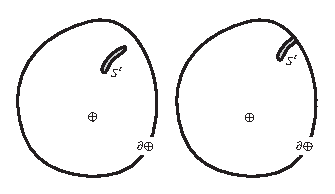
\includegraphics{../figures/chap05/fig01.eps}
\end{center}
\caption[glutvol]{\label{fig5.1}
在光滑的固态地球模型内一个瞬时失效体积
$S^t$ 的示意图。。
\index{source volume}%
\index{volume!source}%
({\em 左图}) 一个完全掩埋的震源,有
$\partial S^t\cap\partial\earth=0$。
({\em 右图}) 一个出露地表的震源,有
$\partial S^t\cap\partial\earth\not=0$}。
\end{wrapfigure}

一般而言,胡克定律的失效在空间上会局限于某个震源区域 $S^t$。这里上角标的作用是提示这一失效过程的时间依赖性;通常,震源会成核于一个点而后灾难性地向周围的点扩散。
瞬时震源体积
\index{source volume}%
\index{volume!source}%
或者完全埋藏在地球内部,或者其表面 $\p S^t$ 也可能与自由表面相交,如图~\ref{fig5.1} 所示。
应力过剩在所有瞬时失效区域以外为零,包括在被掩埋的边界上:
\eq \label{5.Seqzero}
\bS=\bzero\quad\mbox{在 $\earth-S^t$ 内,以及在 $\p S^t-\p S^t\cap\p\earth$ 上。} 
\en
然而要注意的是 $\bS$
在 $\p S^t\cap\p\earth$ 上可能不为零;例如,一个浅部的断层可能延伸至自由表面。

由等效体力和面力密度 $\bef$ 和 $\bt$ 作用在地球上的
{\em 总的力\/}为
\index{force!total}%
\index{total force}%
\eq
\label{5.Fforce}
\bsF=\int_{S^t}\bef\,dV
+\int_{\spar S^t\cap\spar\subearth}\bt\,d\/\Sigma,
\en
此处在表示积分区域时我们使用了两个约束:在 $\earth-S^t$ 内 $\bef=\bzero$, 以及在 $\p\earth-\p S^t\cap\p\earth$ 上 $\bt=\bzero$。 将表达式~(\ref{5.ftforce})
代入~(\ref{5.Fforce}),再使用高斯定理,我们得到
\eq
\label{5.Fforce2}
\bsF=-\int_{\spar S^t-\spar S^t\cap\spar\subearth}
(\bnh\cdot\bS)\,d\/\Sigma.
\en
而作用在地球上的 {\em 总力矩\/} 
\index{total torque}%
\index{torque!total}%
\index{torque}%
\eq
\label{5.Ntorque}
\bsN=\int_{S^t}(\bx\times\bef)\,dV
+\int_{\spar S^t\cap\spar\subearth}(\bx\times\bt)\,d\/\Sigma,
\en
同样可以用应力过剩来表示
\eq \label{5.Ntorque2}
\bsN=\int_{S^t}(\wedge\hspace{0.2 mm}\bS)\,dV-
\int_{\spar S^t-\spar S^t\cap\spar\subearth}
\bx\times(\bnh\cdot\bS)\,d\/\Sigma,
\en
其中 $\wedge$ 是附录~A.1.6中定义的楔形算子。
由于~(\ref{5.Seqzero}) 的条件,(\ref{5.Fforce2})
和~(\ref{5.Ntorque2}) 两式中在掩埋的震源边界
$\p S^t-\p S^t\cap\p\earth$ 上的面积分为零,也因为对称性~(\ref{5.glutsymm}),使得包含 $\wedge\hspace{0.2 mm}\bS$ 的体积分亦为零。
最终,与内部源相应的等效力密度作用在地球上的净力与净力矩均为零:
\eq \label{5.FNzero}
\bsF=\bzero,\qquad\bsN=\bzero.
\en
这个结果是可以预期的,因为任何发生在地球内部及其表面的事件都不可能改变地球的线动量或角动量。

与第4章中的结果一样,非齐次激发问题~(\ref{5.exact4})--(\ref{5.exact5}) 的解可以表示成简正模式的叠加:
\eq
\label{5.response}
\bs(\bx,t)=\Re{\rm e}\sum_k(i\omega_k)^{-1}\bs_k(\bx)\int_{-\infty}^t
C_k(t')\exp i\omega_k(t-t')\,dt',
\en
其中
\eq
\label{5.Csubk}
C_k(t)=\int_{\subearth}\bef(\bx,t)\cdot\bs_k^*(\bx)\,dV
+\int_{\spar\subearth}\bt(\bx,t)\cdot\bs_k^*(\bx)\,d\Sigma.
\en
将~(\ref{5.ftforce}) 中的等效力表达式带入上式,并使用高斯定理,我们可以把式~(\ref{5.Csubk}) 用应力过剩表示成
\eq
\label{5.Csubk2}
C_k(t)=\int_{S^t}\bS(\bx,t)\!:\!\beps_k^*(\bx)\,dV,
\en
这里 $\beps_k=\half[\bdel\bs_k+(\bdel\bs_k)^{\rm T}]$
为与位移本征函数 $\bs_k$ 相应的应变。同样地,
式~(\ref{4.rotaxt}) 所表示的对一个在 $t_0$ 时刻开始并在其后的 $t_{\rm f}$ 时刻达到稳定失效状态的瞬时内在源的加速度响应为
\eq
\label{5.accresp}
\ba(\bx,t)=\Re{\rm e}\sum_kc_k\exp(i\omega_kt)\bs_k(\bx),
\quad t\geq t_{\rm f},
\en
其中
\eq
\label{5.csubk}
c_k=\int_{t_0}^{t_{\rm f}}\int_{S^t}\p_t
\bS(\bx,t)\!:\!\beps
_k^*(\bx)\exp(-i\omega_kt)\,dV\,dt.
\en
式~(\ref{5.Csubk2}) 和~(\ref{5.csubk}) 无论地球有无旋转都是成立的;
$\beps_k^*$ 的星号在无旋情况下是不需要的。
\begin{figure}[!t]
\begin{center}
\scalebox{0.9}{
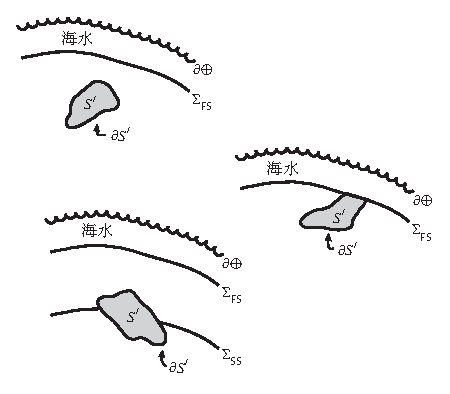
\includegraphics{../figures/chap05/fig02.eps}
}
\end{center}
\caption[3glutvols]{\label{fig5.2}
在较普遍的分段连续地球模型中,震源体积 $S^t$ 可能会出现的三种情况。
\index{source volume}%
\index{volume!source}%
({\em 左上图}) 震源远离任何内部不连续面的完全掩埋,具有 ${\bf t}={\bf 0}$。
({\em 左下图}) 震源跨越内部固-固不连续面,在 $\Sigma_{\rm SS}$ 上具有 ${\bf t}=-[\hat{\bf n}\cdot{\bf S}]^+_-$。  ({\em 右中图}) 震源在固体地球内部但与海底相连,在 $\Sigma_{\rm FS}$ 上具有 ${\bf t}=-[\hat{\bf n}\cdot{\bf S}]^+_-$。}
\end{figure}

上面的结果是在假定地球处处为固态且光滑所得到的;但是它们也同样适用于任何由分段光滑的液态和固态区域所组成的更普遍的地球模型。由于地震都局限于固态的地壳和上地幔,因而应力过剩
$\bS$ 在液态的地核与海洋 $\earth_{\rm F}$ 中为零。当震源区 $S^t$ 跨越内部固-固界面或与海底相交时,如图~\ref{fig5.2}所示,除了作用在 $\p\earth$ 上的外部等效面力密度
$\bt=\bnh\cdot\bS$,还必须考虑 $\Sigma_{\rm SS}$ 和 $\Sigma_{\rm FS}$
上的内部等效面力密度
$\bt=-[\bnh\cdot\bS]^+_-$。
此时需要将高斯定理分别应用于地球的每一个光滑区域,然后把结果合并起来,才能得到正则模式激发表达式
~(\ref{5.Csubk2}) 和~(\ref{5.csubk})。
\index{stress glut|)}%

\section{地震的断层震源}
\index{earthquake fault|(}
\index{source!earthquake fault|(}
\label{5.sec.fault}

一般认为地震是地球内部断层上发生错动的结果。在本节中我们将计算这种地震断层震源的应力过剩 $\bS$ 及其等效体力和面力密度 $\bef$ 和 $\bt$。
我们首先用一个非正规的定性分析来澄清一下应力“过剩”这一名称的来源,然后用分布理论来对一个无穷薄的断层做一个比较正规的处理。

\subsection{基本观念}

我们用一个真实的例子来形象地说明基本观念---考虑一个像加利福尼亚州圣安德列斯断层一样的垂直走滑断层上的地震。我们可以把断层想象为一个很薄的断层泥或破裂带,在地震时发生剧烈形变,而其周围是具有线性弹性的围岩。
定义 $x$ 为右旋滑动方向,$y$ 为断层的法向。
同震滑动量
\index{co-seismic slip}%
\index{slip!co-seismic}%
$s_x$ 与相应的剪应变 $\varepsilon_{xy}=\varepsilon_{yx}=\half(\p_y s_x)$
如图~\ref{fig5.3}所示。
在断层带和围岩内部的模型剪应力均用胡克定律计算,即
$T^{\rm model}_{xy}=T^{\rm model}_{yx}=\mu(\p_y s_x)$,尽管断层泥内的应变已经大到使这一经典的弹性本构关系不再成立。这里我们假定地壳是各向同性的,并且为了避免过于杂乱而省略了表示拉格朗日增量的上脚标L1;我们还假定断层带和围岩具有几乎相同的刚度 $\mu$。
根据连续性条件,在断层泥带内部与周围的弹性围岩中,两者的真实剪应力 $T^{\rm true}_{xy}=T^{\rm true}_{yx}$ 不应相差太大。
在图~\ref{fig5.3}中,我们分别用实线和虚线显示
$T^{\rm model}_{xy}$ 和 $T^{\rm true}_{xy}$
两种应力的变化。如图所示,两者的差
$S_{xy}=T^{\rm model}_{xy}-T^{\rm true}_{xy}$
仅在破裂带内不为零。由于断层带内部过大的非弹性应变而带来过多或“过剩”的模型应力---这正是这一名词的由来。

当破裂带变窄时模型应力增加而真实应力保持基本不变;因此一个窄的垂直走滑断层的应力过剩可以用
$S_{xy}=S_{yx}\approx\mu(\p_y s_x)$ 很好地近似。在无穷薄断层的理想情况下,位移
$s_x$ 趋近于一个阶梯函数,而应力过剩则趋近于狄拉克 $\delta$ 函数:
\eq
\label{5.SanAnd}
S_{xy}=S_{yx}=\mu\Delta s_{\,}\delta(y),
\en
\index{fault slip}%
\index{slip!fault}%
其中 $\Delta s=[s_x]^+_-$ 为断层上的滑动量。
在第~\ref{5.sec.ideal}节我们将会计算在考虑弹性各向异性以及有非流体静力学初始应力时无穷薄的理想断层的应力过剩。
我们将会看到,结果与上面针对各向同性且为流体静力学地球模型所做的启发式分析是一致的。
\begin{figure}[!t]
\begin{center}
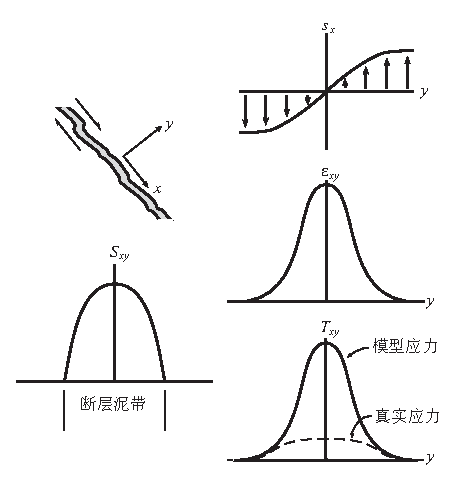
\includegraphics{../figures/chap05/fig03.eps}
\end{center}
\caption[San Andreas]{\label{fig5.3}
({\em 左上图}) 一个垂直的右旋走滑断层的俯视图,图中显示了水平坐标 $x$ 和 $y$。阴影表示理想化的断层泥带,在其内部胡克定律失效。({\em 右上图}) 断层泥带内部位移 $s_x$ 随着与断层的垂直距离 $y$ 的变化。
\index{gouge zone}%
({\em 右中图}) 相应的剪应变 $\varepsilon_{xy}$。  ({\em 右下图}) 模型和真实应力
$T_{xy}$。  ({\em 左下图})  应力过剩
$S_{xy}=T_{xy}^{\rm model}-T_{xy}^{\rm true}$
在断层泥带以外为零。}
\end{figure}

\subsection{分布理论}
\index{distribution theory|(}%

在考虑一般的理想断层之前,对分布理论的一些简单概念做一个回顾是有益的。依照定义,一个 {\em 分布\/}是光滑测试函数
\index{test function}%
空间中的一个连续的线性泛函。
我们用 $\langle f,\varphi\rangle$ 来表示分布
$f$ 给予一个测试函数 $\varphi$ 的标量值。
对于一个处处为光滑固态的地球模型,测试函数在真空空间 $\allspace -\earth$ 中必须为零;更普遍一些,我们要求测试函数在震源所在的地球的固态区域之外均为零。在下面的推导中,我们将指定积分区域为 $\earth$,其边界为 $\p\earth$,同时认识到当存在固-液不连续面时这些区域必须有所修正。在有液态的外核和海洋的地球模型中,可以假定测试函数在地壳与地幔里不为零,而在核幔边界与海底则光滑地趋近于零。

如果我们做如下的定义
\eq
\label{5.dist}
\langle f,\varphi\rangle=\int_{\subearth}f\varphi\,dV,
\en
则任一普通函数 $f$ 也可以被看作是一个分布,其中 $\earth$ 与上述更普遍的解释一致。任何分布,如果只是一个普通函数,而它只有在~(\ref{5.dist}) 的意义上被看作是分布的话,则该分布被称为是
{\em 常规的\/},而其它所有的分布则被称为是 {\em 奇异的\/}。在有必要区分函数与分布时,我们用 $\sD_{\!}f$ 来表示一个与函数 $f$ 相关的常规分布。与此类似,我们也经常会用~(\ref{5.dist}) 的形式来表示由奇异分布 $f$ 赋予 $\varphi$ 的标量;此时,“积分”纯粹是象征性的。

对于一个普通可微分函数 $f$,我们有
\eq
\label{5.byparts}
\int_{\subearth}(\bdel\!f)\varphi\,dV=
-\int_{\subearth}f(\bdel_{\!}\varphi)\,dV,
\en
这里我们使用了高斯定理以及
$\varphi$ 在积分边界 $\p\earth$ 上为零这一条件。与结果~(\ref{5.byparts})对比,我们可以将一个奇异分布 $f$ 的梯度定义为
\eq
\label{5.gradist}
\langle\bdel\!f,\varphi\rangle=-\langle f,\bdel_{\!}\varphi\rangle.
\en
如果测试函数 $\varphi$ 足够光滑,那么在这个意义上所有的分布 $f$ 都可以被微分任意多次。

最为人熟知的奇异分布是
{\em 狄拉克 $\delta$ 分布\/}$\delta_0$,其定义为
\index{Dirac delta distribution}%
\index{distribution!Dirac delta}%
\index{delta function}%
\eq
\label{5.Dirac}
\langle\delta_0,\varphi\rangle=
\int_{\subearth}\delta_0\varphi\,dV=\varphi(\bx_0).
\en
我们将使用~(\ref{5.Dirac})的一个也许人们更为熟悉的形式
\eq
\int_{\subearth}\delta(\bx-\bx_0)_{\,}
\varphi(\bx)\,dV=\varphi(\bx_0).
\en
依照~(\ref{5.gradist})的定义,狄拉克分布的梯度
$\bdel_{\!}\delta_0$ 可以写成
\eqa
\lefteqn{
\langle\bdel_{\!}\delta_0,\varphi\rangle=
\int_{\subearth}\bdel_{\!}
\delta(\bx-\bx_0)_{\,}\varphi(\bx)\,dV} \nonumber \\
&&\mbox{}=-\int_{\subearth}
\delta(\bx-\bx_0)_{\,}\bdel_{\!}\varphi(\bx)\,dV=
-\bdel_{\!}\varphi(\bx_0).
\ena
$\delta(\bx-\bx_0)$ 常常被不太严谨地称作是狄拉克 $\delta$ “函数”。

如果 $w$ 是定义在位于 $\earth$ 内部的表面  
$\Sigma$ 上的一个普通函数,
我们可定义奇异分布 $w\delta_{\Sigma}$ 为
\eq
\label{5.deltaSig}
\langle w\delta_{\Sigma},\varphi\rangle=
\int_{\subearth}(w\delta_{\Sigma})\varphi\,dV=
\int_{\Sigma}w\varphi\,d\/\Sigma.
\en
我们也可以把这一表面狄拉克分布写成一种更明确的形式:
\eq
w\delta_{\Sigma}(\bx)=\int_{\Sigma}w(\bx')_{\,}\delta(\bx-\bx')
\,d\/\Sigma'.
\en
我们可以把 $w\delta_{\Sigma}$ 看作是狄拉克 $\delta$ 函数在表面 $\Sigma$ 上的一个加权
“分布”, 正如我们把
$\sum_kw_k\delta(\bx-\bx_k)$ 看作是加权的离散“分布”。
$w\delta_{\Sigma}$ 的值在 $\Sigma$ 以外处处为零,
如同 $\sum_kw_k\delta(\bx-\bx_k)$ 的值一样,除了在
$\bx_k$ 点以外处处为零(一个奇异分布的逐点取值这一直观上易于理解的概念可以通过考虑测试函数 $\varphi$ 的支撑来严格定义)。
狄拉克梯度的加权“分布”
\eq
w\bdel_{\!}\delta_{\Sigma}(\bx)=
\int_{\Sigma}w(\bx')_{\,}\bdel_{\!}\delta(\bx-\bx')\,d\/\Sigma'
\en
对于任一测试函数 $\varphi$ 具有可复制性
\eq
\langle w\bdel_{\!}\delta_{\Sigma},\varphi\rangle=
-\int_{\Sigma}w(\bdel_{\!}\varphi)\,d\/\Sigma.
\en

\begin{figure}[t]
\begin{center}
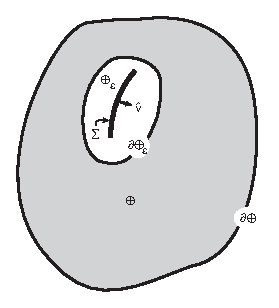
\includegraphics{../figures/chap05/fig04.eps}
\end{center}
\caption[punctvol]{\label{fig5.4}
图中阴影表示公式~(\ref{5.proof2}) 中的积分体积
$\earth-\earth_{\varepsilon}$。在
$\varepsilon\rightarrow 0$ 的极限情形,内边界
$\partial\earth_{\varepsilon}$ 收缩到包覆的不连续面 $\Sigma$ 上。}
\end{figure}

我们现在假设 $f$ 是一个在
$\earth$ 内处处光滑的函数,只有在一个包覆于内部的表面 $\Sigma$ 上有一个不连续跃变 $[f]^+_-$。
$f$ 的梯度作为一个普通函数在 $\earth$ 内部不存在,尤其是在 $\Sigma$ 上。但是,我们可以计算与之相应的常规分布 $\sD_{\!}f$ 的梯度。
要计算 $\bdel(\sD_{\!}f)$,我们来考虑它赋予一个任意测试函数的标量:
\eq
\label{5.proof}
\langle\bdel(\sD_{\!}f),\varphi\rangle=
-\langle\sD_{\!}f,\bdel_{\!}\varphi\rangle.
\en
我们可以把~(\ref{5.proof}) 右边的量看作是在一个去除了不连续面之后的有缝的体积
$\earth-\earth_{\varepsilon}$ 内普通积分的极限值:
\eq
\label{5.proof2}
\langle\bdel(\sD_{\!}f),\varphi\rangle=
-\lim_{\varepsilon\rightarrow 0}
\int_{\subearth-\subearth_{\varepsilon}}
f(\bdel_{\!}\varphi)\,dV.
\en
如图~\ref{fig5.4} 所示,积分体积 $\earth-\earth_{\varepsilon}$ 内部的表面 $\p\earth_{\varepsilon}$ 完全包覆了
$\Sigma$,而且在取
$\varepsilon\rightarrow 0$ 的极限时收缩到 $\Sigma$ 上。在取极限之前可以对
~(\ref{5.proof2}) 中的积分使用高斯定理。
由于 $\varphi$ 在 $\p\earth$ 上为零,我们得到
\eq
\label{5.proof3}
\langle\bdel(\sD_{\!}f),\varphi\rangle=
\int_{\subearth}
(\bdel\!f)\varphi\,dV
+\int_{\Sigma}\bnuh[f]^+_{-\,}\varphi\,d\/\Sigma,
\en
其中 $\bnuh$ 是表面 $\Sigma$ 的单位法向矢量。
式~(\ref{5.proof3}) 右边体积分中的函数 $\bdel\!f$ 一般在跨过表面 $\Sigma$ 时是不连续的;从分布理论的角度,它在 $\Sigma$ {\em 之上\/} 的值是无关紧要的。
把 $\bdel\!f$ 用相应的常规分布
$\sD(\bdel\!f)$ 替代,并利用~(\ref{5.deltaSig}) 的定义,我们得到
\eq
\label{5.proof4}
\langle\bdel(\sD_{\!}f),\varphi\rangle=\langle
\sD(\bdel\!f)+\bnuh[f]^+_{-\,}\delta_{\Sigma},\varphi\rangle.
\en
式~(\ref{5.proof4}) 表明 $\bdel(\sD_{\!}f)$
和 $\sD(\bdel\!f)+\bnuh[f]^+_{-\,}\delta_{\Sigma}$ 
赋予每一个测试函数 $\varphi$ 相同的标量;因而它们一定是同一个奇异分布:
\index{distribution!gradient of}%
\index{gradient!of a distribution}%
\eq
\label{5.delsDf}
\bdel(\sD_{\!}f)=\sD(\bdel\!f)+\bnuh[f]^+_{-\,}\delta_{\Sigma}.
\en
用一个不够严谨的说法, 式~(\ref{5.delsDf}) 的结果表明 $f$ 的梯度处处是“普通”梯度 $\bdel\!f$,除了在表面 $\Sigma$ 上会有因不连续跃变 $[f]^+_-$ 而产生的一个额外的 $\delta$-函数贡献。
我们也许对以下一维而非三维的类似结果更加熟悉:
\eq \label{5.1Dderiv}
d(\sD_{\!}f)\hspace{-0.1 mm}/\hspace{-0.1 mm}dx=
\sD(df\hspace{-0.3 mm}/\hspace{-0.2 mm}dx)
+[f]^+_{-\,}\delta_0.
\en
式~(\ref{5.1Dderiv})中的函数 $f$ 处处光滑,只有在  $x=x_0$ 处有一个不连续的跃变 $[f]^+_-$。它的导数
$d(\sD_{\!}f)\hspace{-0.1 mm}/\hspace{-0.1 mm}dx$
包含一个“普通”贡献
$\sD(df\hspace{-0.3 mm}/\hspace{-0.2 mm}dx)$ 和一个 奇异贡献 $[f]^+_{-\,}\delta_0$。
\index{distribution theory|)}%

\subsection{理想断层}
\index{ideal fault|(}%
\index{fault!ideal|(}%
\label{5.sec.ideal}

一个 {\em 理想断层\/}是 $\earth$ 内的一个表面 $\Sigma^t$,跨过该表面有一个切向的不连续滑动 $\bDelta\bs=[\bs]^+_-$。断层面的两侧不容许分离或相互穿透,因而我们有
\eq
\bnuh\cdot\bDelta\bs=0\quad\mbox{on $\Sigma^t$.}
\en
此外,滑动 $\bDelta\bs$ 在瞬时的断层边缘 $\p\Sigma^t$ 上必须为零,除非在该边缘与固体地表或海底相交的地方。
$\Sigma^t$ 和 $\p\Sigma^t$ 的上角标表示发生破裂的区域一般是随时间变化的,
因为滑动会以一个点为核心向外扩展。
我们假设在地球内部线性弹性本构关系
$\bT^{\rm L1}=\bUpsilon\!:\!\bdel\bs$ 除了在 $\Sigma^t$ 面以外处处成立。因此,可以认为胡克定律的失效仅局限于无穷薄的断层上。

真实的物理应力 $\bT^{\rm L1}_{\rm true}$
\index{stress!true}%
\index{true stress}%
在跨越断层时一般是不连续的,但是相应的分布
$\sD(\bT^{\rm L1}_{\rm true})$ 是常规的:
\eq
\sD(\bT^{\rm L1}_{\rm true})=\bUpsilon\!:\!\sD(\bdel\bs).
\en
然而胡克模型应力却是奇异分布
\index{stress!model}%
\index{model stress}%
\index{stress!Hooke}%
\index{Hooke stress}%
\eq
\label{5.modstress}
\bT^{\rm L1}_{\rm model}=\bUpsilon\!:\!\bdel(\sD\bs).
\en
应力过剩,即模型与真实应力之间的差 $\bT^{\rm L1}_{\rm model}
-\sD(\bT^{\rm L1}_{\rm true})$ 很明显是
\eq \label{5.Seqdiff}
\bS=\bUpsilon\!:\![\bdel(\sD\bs)
-\sD(\bdel\bs)]=(\bUpsilon\!:\!\bnuh\bDelta\bs)\delta_{\Sigma^t},
\en
这里我们使用了分布的求导关系~(\ref{5.delsDf})。为方便起见,可以定义断层面上的 {\em 应力过剩密度\/}
\index{stress glut density}%
\eq
\label{5.mdef}
\bm=\bUpsilon\!:\!\bnuh\bDelta\bs.
\en
利用应力过剩密度,我们可以把~(\ref{5.Seqdiff}) 写成
\eq
\label{5.GLUT}
\bS=\bm\hspace{0.2 mm}\delta_{\Sigma^t}.
\en
(\ref{5.GLUT}) 中的理想断层的应力过剩是一个奇异分布,它除了在胡克定律失效的断层面 $\Sigma^t$ 上不为零以外,在其它地方处处为零。
$\bm$ 这个量也被称为
{\em 表面地震矩密度张量\/},
\index{tensor!surface moment-density}%
\index{surface moment-density tensor}%
它是滑动断层的无穷小面元上单位面积的应力过剩。
在一个普遍各向异性地球模型中,四阶张量
$\bUpsilon$ 与弹性张量 $\bGamma$ 之间有一定关系 
$\Upsilon_{ijkl}=\Gamma_{ijkl}+\half(-T^{\,0}_{ij\,}\delta_{kl}
+T^{\,0}_{kl\,}\delta_{ij}+T^{\,0}_{ik\,}\delta_{jl}+T^{\,0}_{jk\,}\delta_{il}
-T^{\,0}_{il\,}\delta_{jk}-T^{\,0}_{jl\,}\delta_{ik})$。
一个不连续函数与狄拉克分布的乘积是没有定义的;因此,有必要要求在跨越断层时 $\bUpsilon$ 是连续的:
\eq
[\bUpsilon]^+_-=\bzero\quad\mbox{在 $\Sigma^t$ 上.}
\en
(\ref{5.GLUT}) 在断层与海底相交或穿过固-固不连续面时成立;但是,由于上式的条件,它不适用于断层与 $\Sigma_{\rm SS}$ 的一部分有重叠的情形。

利用~(\ref{5.ftforce}) 得到的等效体力与面力密度是
\index{force!body}%
\index{body force}%
\index{surface force}%
\index{force!surface}%
\eq
\label{5.ftforce2}
\bef=-\bm\cdot\bdel_{\!}\delta_{\Sigma^t}\quad\mbox{在 $\earth$ 内},\qquad
\bt=(\bnh\cdot\bm)_{\,}\delta_{\Sigma^t}\quad\mbox{在 $\p\earth$ 上}.
\en
体力密度 $\bef$ 在瞬时断层面 $\Sigma^t$ 之外处处为零,而面力密度 $\bt$ 也在可见的破裂迹线 $\p\Sigma^t\cap\p\earth$ 之外处处为零。
很容易证明~(\ref{5.ftforce2}) 中的等效力作用在地球上的净力与净力矩满足~(\ref{5.FNzero}) 的约束。
由于表面地震矩密度张量的对称性:$\bm^{\rm T}=\bm$,力矩 $\bsN$ 为零。
该对称性同时保证 $\bm$ 总是能够写成对角的形式:
\eq
\bm=m_+\beh_+\beh_++m_0\beh_0\beh_0+m_-\beh_-\beh_-,
\en
其中 $m_+ \geq m_0 \geq m_-$ 为本征值,
$\beh_+$, $\beh_0$, $\beh_-$ 为相应的归一化本征矢量。
如图~\ref{fig5.5} 所示,等效体力密度 
$\bef$ 可以被看作是分布在 $\Sigma^t$ 上的互相垂直的
{\em 线矢量偶极子\/},
\index{linear vector dipole}%
其强度分别为 $m_+$,$m_0$,$m_-$。
本征值为正的偶极子方向“向外”,本征值为负的偶极子方向“向内”。

在一个具有流体静力学初始应力的各向同性地球模型中,张量 $\bUpsilon$ 可以写成 
$\Upsilon_{ijkl}=\Gamma_{ijkl}=(\kappa-\twothirds\mu)
\delta_{ij\,}\delta_{kl}+\mu(\delta_{ik\,}\delta_{jl}
+\delta_{il\,}\delta_{jk})$,
其中 $\kappa$ 是等熵不可压缩性,$\mu$ 是刚度。表面地震矩密度张量~(\ref{5.mdef}) 可因此简化为
\eq
\label{5.mhydro}
\bm=\mu\Delta s(\bnuh\bsigmah+\bsigmah\bnuh),
\en
其中 $\Delta s$ 是滑动矢量的大小, $\bsigmah$
为其方向,即 $\bDelta\bs=\Delta s_{\,}\bsigmah$。
各向同性地球模型中的等效体力密度 $\bef$ 可被视为断层面 $\Sigma^t$ 上的
{\em 双力偶\/}分布;
\index{double couple}%
\index{source!double-couple}%
这一为人熟知的表述已经在许多地震学研究中得到应用。另外,我们也可以把 $\bm$ 写成对角的形式
\eq
\bm=\mu\Delta s(\beh_+\beh_+-\beh_-\beh_-),
\en
其中 $\beh_{\pm}=(\bnuh\pm\bsigmah)/\!\sqrt{2}$,
同时把 $\bef$ 看作是大小相等、方向相反的线矢量偶极子分布,
如图~\ref{fig5.5} 所示。如同所预期的,
(\ref{5.mhydro}) 中的表述与前面得到的垂直走滑断层的结果~(\ref{5.SanAnd}) 一致。
\begin{figure}[!t]
\begin{center}
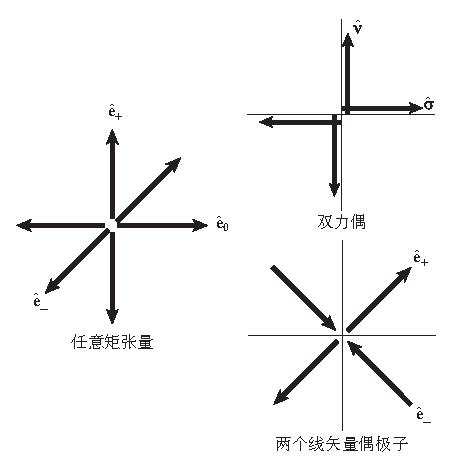
\includegraphics{../figures/chap05/fig05.eps}
\end{center}
\caption[equivforces]{\label{fig5.5}
({\em 左图}) 与任意地震矩密度张量 ${\bf m}$ 相应的等效体力密度 ${\bf f}$。 很明显,这种线矢量偶极子分布对地球的净力和净力矩作用均为零。
\index{linear vector dipole}%
({\em 右图}) 在具有流体静力学初始应力的各向同性地球中,${\bf f}$ 可以被想象成是地震矩为
$\mu\Delta s$ 的反向力偶分布,即双力偶
({\em 右上图\/}),也可以是与断层面夹 $45^{\circ}$ 角的两个互相垂直的线矢量偶极子分布 ({\em 右下图\/})。}
\end{figure}

一个理想断层源产生的位移可以用表面地震矩张量密度表示为
\eq
\label{5.faultresp}
\bs(\bx,t)=\Re{\rm e}\sum_k(i\omega_k)^{-1}\bs_k(\bx)\int_{-\infty}^t
C_k(t')\exp i\omega_k(t-t')\,dt',
\en
其中
\eq
\label{5.Csubkfault}
C_k(t)=\int_{\Sigma^t}\bm(\bx,t)\!:\!\beps_k^*(\bx)\,d\Sigma.
\en
同样地,破裂停止后的加速度响应可以写成
\eq
\label{5.faultacc}
\ba(\bx,t)=\Re{\rm e}\sum_kc_k\exp(i\omega_kt)\bs_k(\bx),
\quad t\geq t_{\rm f},
\en
其中
\eq
\label{5.csubkfault}
c_k=\int_{t_0}^{t_{\rm f}}\int_{\Sigma^t}
\p_t\bm(\bx,t)\!:\!\beps_k^*(\bx)
\exp(-i\omega_kt)\,d\Sigma\,dt.
\en
上述结果只要将~(\ref{5.GLUT})
代入普遍公式~(\ref{5.response})--(\ref{5.csubk}) 中即可得到。

以上推导固然给人一种奇异的感觉;但数学支撑一旦建立,~(\ref{5.ftforce2}) 的等效力表述就像凭空出现一样轻松地获得。我们已经尽可能地在讨论中以物理意义为主,但是,必须承认,对于初学者来说,应力过剩并不是一个容易理解的物理概念。特别是很难设想出一个能够由实验家设计制造的“应力过剩测量仪”。由于这一原因,同时考虑到~(\ref{5.ftforce2}) 结果的重要性,在继续讨论之前,我们用一个更传统的方法再把它推导一遍。。
\index{ideal fault|)}%
\index{fault!ideal|)}%
\index{earthquake fault|)}
\index{source!earthquake fault|)}

\renewcommand{\thesection}{$\!\!\!\raise1.3ex\hbox{$\star$}\!\!$
\arabic{chapter}.\arabic{section}}
\section{Burridge-Knopoff方法}
\index{Burridge-Knopoff method|)}%
\label{5.sec.Green}
\renewcommand{\thesection}{\arabic{chapter}.\arabic{section}}

欲得到在施加体力密度 $\bef$ 和表面牵引力 $\bt$ 时所产生的位移 $\bs$,我们需要解下列方程组
\eqa
\label{5.lineqn1}
\lefteqn{\rho^0(\p_t^2\bs+2\bOmega\times\p_t\bs)-\bdel\cdot\bT^{\rm PK1}}
\nonumber \\
&&\mbox{}+\rho^0\bdel\phi^{\rm E1}+\rho^0\bs\cdot\bdel\bdel(\phi^0+\psi)=\bef
\quad\mbox{在 $\earth$ 内},
\ena
\eq
\label{5.lineqn2}
\bnh\cdot\bT^{\rm PK1}=\bt\quad\mbox{在 $\p\earth$ 上},
\en
\eq
\label{5.lineqn3}
[\bnh\cdot\bT^{\rm PK1}]^+_-=\bzero\quad\mbox{在 $\Sigma_{\rm SS}$ 上},
\en
\eq
\label{5.lineqn4}
[\bt^{\rm PK1}]^+_-=\bnh[\bnh\cdot\bt^{\rm
PK1}]^+_-=\bzero\quad\mbox{在 $\Sigma_{\rm FS}$ 上}.
\en
同样地,对另外一组作用力密度 $\overline{\bef}$ 和 $\overline{\bt}$,以相反的角速度 $\bOmega\rightarrow -\bOmega$ 自转的逆转地球的响应
$\overline{\bs}$ 
可以通过求解下列方程组而得到
\index{force!body}%
\index{body force}%
\index{surface force}%
\index{force!surface}%
\eqa
\label{5.lineqn5}
\lefteqn{\rho^0(\p_t^2\overline{\bs}-2\bOmega
\times\p_t\overline{\bs})-\bdel\cdot\overline{\bT}
^{\,\raise-.45ex\hbox{\scriptsize\rm PK1}}}
\nonumber \\
&&\mbox{}+\rho^0\bdel\overline{\phi}
^{\,\raise-.5ex\hbox{\scriptsize\rm E1}}+\rho^0
\overline{\bs}\cdot\bdel\bdel(\phi^0+\psi)=\overline{\bef}
\quad\mbox{在 $\earth$ 内},
\ena
\eq
\label{5.lineqn6}
\bnh\cdot\overline{\bT}^{\,\raise-.45ex\hbox{\scriptsize\rm PK1}}
=\overline{\bt}\quad\mbox{在 $\p\earth$ 上},
\en
\eq
\label{5.lineqn7}
[\bnh\cdot\overline{\bT}^{\,\raise-.45ex\hbox{\scriptsize\rm PK1}}]^+_-
=\bzero\quad\mbox{在 $\Sigma_{\rm SS}$ 上},
\en
\eq
\label{5.lineqn8}
[^{\,}\overline{\bt}^{\,\raise-.45ex\hbox{\scriptsize\rm PK1}}]^+_-
=\bnh[\bnh\cdot\overline{\bt}^{\,\raise-.45ex\hbox{\scriptsize\rm PK1}}]^+_-
=\bzero\quad\mbox{在 $\Sigma_{\rm FS}$ 上}.
\en
我们将 $\overline{\bs}$ 与动量方程~(\ref{5.lineqn1}) 做点乘,以及将 $\bs$ 
与逆转地球动量方程~(\ref{5.lineqn5}) 做点乘,并在地球模型 $\earth$ 上积分,同时使用高斯定理。
与前面的推导一样,在
$\p\earth\cup\Sigma_{\rm SS}\cup\Sigma_{\rm FS}$
上包含跃变 $[\bnh\cdot\bT^{\rm PK1}\cdot\overline{\bs}^{\,}]^+_-$ 和
$[\bnh\cdot\overline{\bT}^{\,\raise-.45ex\hbox{\scriptsize\rm
PK1}}\cdot\bs]^+_-$ 的面积分以及体积分中的厄密特项均被消掉,只剩下
\eqa
\label{5.Betti}
\lefteqn{\int_{\subearth}[\rho^0\overline{\bs}
\cdot\p_t^2\bs+2\rho^0\overline{\bs}
\cdot(\bOmega\times\p_t\bs)-\overline{\bs}\cdot\bef]\,dV
-\int_{\spar\subearth}\overline{\bs}\cdot\bt\,d\/\Sigma} \\
&&\mbox{}=\int_{\subearth}[\rho^0\bs\cdot\p_t^2\overline{\bs}-2\rho^0\bs
\cdot(\bOmega\times\p_t\overline{\bs})-\bs\cdot\overline{\bef}]\,dV
-\int_{\spar\subearth}\bs\cdot\overline{\bt}\,d\/\Sigma. \nonumber
\ena

方程~(\ref{5.Betti}) 中即使有上横线和无上横线的量是在不同时刻的取值该方程也是成立的;为方便起见,可以假定 $\bef$, $\bt$, $\bs$ 均在 $t$ 时刻取值,
而 $\overline{\bef}$, $\overline{\bt}$, $\overline{\bs}$ 均在 $-t$ 时刻取值。在
$-\infty\leq t\leq \infty$ 上对时间做分部积分,我们得到
\eqa
\label{5.Betti2}
\lefteqn{\int_{-\infty}^{\infty}\int_{\subearth}\bs(\bx,t)\cdot
\overline{\bef}(\bx,-t)\,dV\,dt} \nonumber \\
&&\mbox{}+\int_{-\infty}^{\infty}\int_{\spar\subearth}
\bs(\bx,t)\cdot\overline{\bt}(\bx,-t)\,d\/\Sigma\,dt \nonumber \\
&&\mbox{}\qquad
=\int_{-\infty}^{\infty}\int_{\subearth}\overline{\bs}(\bx,-t)\cdot
\bef(\bx,t)\,dV\,dt \nonumber \\
&&\mbox{}\qquad\qquad\qquad+\int_{-\infty}^{\infty}\int_{\spar\subearth}
\overline{\bs}(\bx,-t)\cdot\bt(\bx,t)\,d\/\Sigma\,dt.
\ena
我们可以假定力 $\bef$, $\bt$ 和
$\overline{\bef}$, $\overline{\bt}$ 都是逐渐开启的,或者是从过去某个有限的时刻开始的,因而根据因果条件,来自
$\pm\infty$ 的贡献均为零。
公式~(\ref{5.Betti2}) 是经典的 {\em Betti 互易性关系\/}在自转、自引力地球情形的推广。
\index{Betti reciprocal relation}%
\index{reciprocity!Betti}%
值得注意的是,它同时依赖于逆转地球以及实际地球。 

现在假设两个施加的表面牵引力均为零,即
$\bt=\overline{\bt}=\bzero$,
同时两个体力均为脉冲点力:
\eq
\bef(\bx,t)=\bxh_{q\,}\delta(\bx-\bx')_{\,}\delta(t-t'),
\en
\eq
\label{5.fbar}
\overline{\bef}(\bx',t')=\bxh_{p\,}\delta(\bx'-\bx)_{\,}\delta(t'+t).
\en
此时所对应的响应可以用格林张量 $\bG$ 和逆转地球格林张量 $\overline{\bG}$ 表示成
\eq
s_p(\bx,t)=G_{pq}(\bx,\bx';t-t'),
\en
\eq
\label{5.Greenbar}
\overline{s}_q(\bx',t')=\overline{G}_{qp}(\bx',\bx;t'+t).
\en
Betti关系~(\ref{5.Betti2}) 简化为
$s_p(\bx,t)=\overline{s}_q(\bx',-t')$,或者等效于
\eq
\label{5.recip}
\bG(\bx,\bx';t-t')=\overline{\bG}^{\,\rm T}(\bx',\bx;t-t').
\en
公式~(\ref{5.recip}) 正是我们在前面第~4.2.6节所建立的 {\em 广义源点-接收点互易性原理\/}。
\index{reciprocity!generalized}%
\index{generalized reciprocity}%

取 $\overline{\bt}$ 为零, $\overline{\bef}$
为~(\ref{5.fbar}) 的脉冲形式,但令
$\bef$ 和 $\bt$ 为任意形式,我们有
\eqa
\label{5.Greenrep}
\lefteqn{
\bs(\bx,t)=\int_{-\infty}^t\int_{\subearth}\overline{\bG}^{\,\rm T}
(\bx',\bx;t-t')\cdot\bef(\bx',t')\,dV'\,dt'} \nonumber \\
&&\mbox{}\qquad\qquad+\int_{-\infty}^t\int_{\spar\subearth}
\overline{\,\bG}^{\,\rm T} (\bx',\bx;t-t')\cdot\bt(\bx',t')\,d\/\Sigma'\,dt',
\ena
这里我们看到了~(\ref{5.Greenbar}),
并且利用了逆转地球格林张量
$\overline{\bG}(\bx,\bx';t-t')$ 在 $t<t'$ 时为零的特性。利用互易性关系~(\ref{5.recip}),我们可以从式~(\ref{5.Greenrep}) 中消去所有对逆转地球的依赖性:
\eqa
\label{5.Greenrep2}
\lefteqn{
\bs(\bx,t)=\int_{-\infty}^t\int_{\subearth}\bG
(\bx,\bx';t-t')\cdot\bef(\bx',t')\,dV'\,dt'} \nonumber \\
&&\mbox{}\qquad\qquad+\int_{-\infty}^t\int_{\spar\subearth}\bG
(\bx,\bx';t-t')\cdot\bt(\bx',t')\,d\/\Sigma'\,dt'.
\ena
公式~(\ref{5.Greenrep2}) 以同格林张量做卷积的形式给出了对施加的力 $\bef$
和 $\bt$ 的响应 $\bs$。在第~4.2.7节中我们将利用这一直观上显而易见的结果把同一响应表示为正则模式的叠加。

我们接下来假设施加的面力 $\bt$ 和 $\overline{\bt}$ 为零,但是在地球内部有断层面 $\Sigma^t$,跨过该面位移 
$\bs$ 和 $\overline{\bs}$ 可以不连续。重复我们推导
~(\ref{5.Betti2}) 所采用的思路,可以得到
\eqa
\label{5.Betti3}
\lefteqn{\int_{-\infty}^{\infty}\int_{\subearth}\bs(\bx,t)\cdot
\overline{\bef}(\bx,-t)\,dV\,dt} \nonumber \\
&&\mbox{}-\int_{-\infty}^{\infty}\int_{\Sigma^t}
[\bnuh(\bx)\cdot\overline{\bT}^{\,\raise-.45ex\hbox{\scriptsize\rm PK1}}
(\bx,-t)\cdot\bs(\bx,t)]^+_-\,d\/\Sigma\,dt = \nonumber \\
&&\mbox{}\!\!\!\!\!\!\!\!\!\!\!\!\!\!\!
\int_{-\infty}^{\infty}\int_{\subearth}\overline{\bs}(\bx,-t)\cdot
\bef(\bx,t)\,dV\,dt
\nonumber \\
&&\mbox{}-\int_{-\infty}^{\infty}\int_{\Sigma^t}
[\bnuh(\bx)\cdot\bT^{\rm PK1}
(\bx,t)\cdot\overline{\bs}(\bx,-t)]^+_-\,d\/\Sigma\,dt,
\ena
上式为Betti互易性关系的推广。
\index{Betti reciprocal relation}%
\index{reciprocity!Betti}%
式~(\ref{5.Betti3}) 中的面积分并不为零,这一点与固-液边界
$\Sigma_{\rm FS}$ 上相应的积分并不相同,因为在断层面
$\Sigma^t$ 上并不是没有摩擦力的。要使~(\ref{5.Betti3}) 成立并不需要假定断层是完全处于地壳或上地幔的某个光滑区域内部。如果 $\Sigma^t$ 与固态自由表面 $\p\earth$ 或海底 $\Sigma_{\rm FS}$ 相交,或是穿过一个固-固不连续面 $\Sigma_{\rm SS}$,那么就必须在积分时如图~\ref{fig5.6}所示使用高斯定理。

为了应用~(\ref{5.Betti3}) 我们再次取
$\overline{\bef}$
为~(\ref{5.fbar}) 一样的单位脉冲形式,并取
$\bef$ 为零;将位移 $\bs$ 看作是对断层破裂的响应。
借助广义互易性关系~(\ref{5.recip})
以及Maxwell关系 $\Lambda_{ijkl}=\Lambda_{klij}$ 将逆转地球中的位移 $\overline{\bs}$ 和其相关的应力 $\overline{\bT}^{\,\raise-.70ex\hbox{\scriptsize\rm PK1}}$
用格林张量 $\bG$ 表示,我们得到
\eqa
\label{5.Betti4}
\lefteqn{
s_p(\bx,t)=\int_{-\infty}^{t}\int_{\Sigma^t}[\p^{\prime}_iG_{pj}
(\bx,\bx';t-t')\Lambda_{ijkl}(\bx')\nu_k(\bx')s_l(\bx',t')} \nonumber \\
&&\mbox{}\qquad\quad-G_{pj}(\bx,\bx';t-t')\nu_i(\bx')T_{ij}^{\rm PK1}(\bx',t')]^+_-
\,d\/\Sigma'\,dt',
\ena
其中 $\p^{\prime}_i$ 代表对坐标 $x_i^{\prime}$ 的偏导数。牵引力增量
$\bnuh\cdot\bT^{\,\raise-.45ex\hbox{\scriptsize\rm PK1}}$
满足线性化的动力学边界条件~(\ref{3.slipbc}),该条件可以写成更方便的角标形式:
\eq
\label{5.slipbc}
[\nu_iT^{\rm PK1}_{ij}]^+_-=[\p^{\Sigma}_i(s_i\nu_kT^0_{kj})]^+_-,
\en
这里 $\p^{\Sigma}_i=\p_i-\nu_i(\nu_j\p_j)$。
利用式~(\ref{5.slipbc}) 以及附录中的二维形式的高斯定理~(\ref{A.2DGauss})--(\ref{A.2DGauss2}),我们可以把~(\ref{5.Betti4}) 右边的第二项表示成
\eqa
\label{5.twoDGauss}
\lefteqn{
\int_{\Sigma^t}[G_{pj}\nu_i
T_{ij}^{\rm PK1}]^+_-\,d\/\Sigma'
=\int_{\spar\Sigma^t_{\rm c}}
G_{pj}[\nu_kT^0_{kj}
b_is_i]^+_-\,dL'} \nonumber \\
&&\mbox{}\qquad\qquad-\int_{\Sigma^t}
\p^{\prime}_iG_{pj}[\nu_k
T^0_{kj}s_i]^+_-\,d\/\Sigma',
\ena
其中 $\bbh$ 为在 $\p\Sigma^t$ 上与 $\Sigma^t$ 相切且指向 $\Sigma^t$ 外部的单位法向矢量。
公式~(\ref{5.twoDGauss}) 中的线积分只需在掩埋部分的断层边界上计算,那里积分面折叠在自身上面,如图\ref{fig5.6}所示;在这种瞬时破裂前缘或 {\em 断裂尖端\/} $\p\Sigma^t_{\rm c}$,滑动量 $\bDelta\bs$ 趋于零,因而其贡献为零。
\index{crack tip}%
\index{rupture front}%
\begin{figure}[!t]
\begin{center}
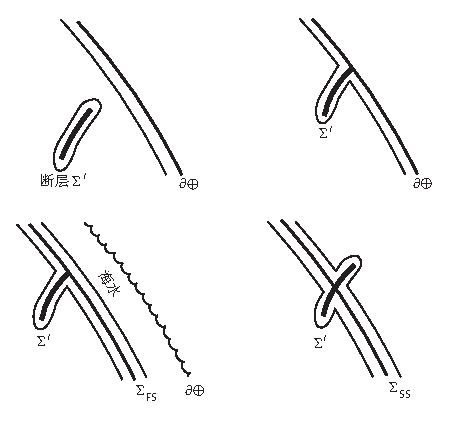
\includegraphics{../figures/chap05/fig06.eps}
\end{center}
\caption[integrationpaths]{\label{fig5.6}
在推导广义Betti互易性关系~(\ref{5.Betti3}) 中积分处理的示意图。细线表示在使用高斯定理时必须考虑的积分面;在每一种情形中,可以想象这些面都需要变形,以使积分区域为整个地球 $\earth$。  ({\em 左上图}) 若断层完全掩埋于地球 $\earth$ 的一个光滑的固态区域内,则积分面包括自由表面 $\partial\earth$ 的外侧和 $\Sigma^t$ 的双侧。  ({\em 右上图}) 若断层面与固态自由表面相交,则积分面必须以“单侧”方式包覆住 $\Sigma^t$;此时出露的断层迹线 $\partial\Sigma^t\cap\partial\earth$ 对~(\ref{5.twoDGauss}) 中的线积分没有贡献。 ({\em 右下图})
若断层穿过一个固-固不连续面,则积分面必须把
$\Sigma^t$ 和 $\Sigma_{\rm SS}$ 同时包覆住。
({\em 左下图}) 如果断层与海底相交,则 $\partial\Sigma^t\cap\Sigma_{\rm FS}$ 对
~(\ref{5.twoDGauss}) 中的线积分没有贡献。}
\end{figure}
将~(\ref{5.Betti4}) 和~(\ref{5.twoDGauss}) 中剩下的面积分合并,再利用弹性张量关系式~(\ref{3.GamXi}) ,我们可以把对 $\Sigma^t$ 上给定滑动分布 
$\bDelta\bs$ 的响应写成一个简洁的形式
\eq
\label{5.Volt}
s_p(\bx,t)=\int_{-\infty}^{t}
\int_{\Sigma^t}\p^{\prime}_iG_{pj}(\bx,\bx';t-t')
m_{ij}(\bx',t')\,d\/\Sigma'\,dt',
\en
其中 $\bm=\bUpsilon\!:\!\bnuh\bDelta\bs$ 是表面地震矩密度张量。
在~(\ref{5.Volt}) 的推导中,我们假定初始静态应力在断层两侧是连续的,即
$[\bT^0]^+_-=\bzero$,同时使用了运动学边界条件
$\bnuh\cdot\bDelta\bs=0$。我们还假定了格林张量及其梯度是连续的,即 $[\bG]^+_-=\bzero$ 和
$[\bdel^{\prime}\bG]^+_-=\bzero$。由于后一个限制,断层面不能与 $\Sigma_{\rm SS}$ 有重叠的部分。
将位移 $\bs$ 用 $\bm$ 表示的公式
~(\ref{5.Volt}) 有时候被称为
{\em Volterra 表述定理\/}。
\index{Volterra representation theorem}%

为了确定等效体力和面力密度 $\bef$ 和 $\bt$,我们把格林张量的梯度改写为
\eqa
\label{5.GreeDir}
\lefteqn{
\p^{\prime}_iG_{pj}(\bx,\bx';t-t')=\int_{\subearth}
\delta(\bx''-\bx')_{\,}\p_i^{\prime\prime}
G_{pj}(\bx,\bx'';t-t')\,dV''}
\nonumber \\
&&\mbox{}=\int_{\spar\subearth}\delta(\bx''-\bx')_{\,}
n_i(\bx'')G_{pj}(\bx,\bx'';t-t')\,d\/\Sigma'' \nonumber \\
&&\mbox{}\qquad\qquad-\int_{\subearth}
\p^{\prime\prime}_i\delta(\bx''-\bx')_{\,}G_{pj}(\bx,\bx'';t-t')\,dV'',
\ena
其中 $\delta(\bx''-\bx')$ 是狄拉克分布。
将~(\ref{5.GreeDir}) 代入Volterra
表述~(\ref{5.Volt}),我们有
\eqa
\label{5.Greenft}
\lefteqn{\bs(\bx,t)=\int_{-\infty}^t\int_{\subearth}
\bG(\bx,\bx';t-t')\cdot\bef(\bx',t')\,dV'\,dt'} \nonumber \\
&&\mbox{}\qquad\qquad+\int_{-\infty}^t\int_{\spar\subearth}
\bG(\bx,\bx';t-t')\cdot\bt(\bx',t')\,d\/\Sigma'\,dt',
\ena
其中
\eq
\label{5.fForce}
\bef(\bx,t)=-\int_{\Sigma^t}\bm(\bx',t)\cdot
\bdel_{\!}\delta(\bx-\bx')
\,d\/\Sigma'\quad\mbox{在 $\earth$ 内},
\en
\eq
\label{5.tForce}
\bt(\bx,t)=\bnh(\bx)\cdot\int_{\Sigma^t}\bm(\bx',t)_{\,}
\delta(\bx-\bx')
\,d\/\Sigma'\quad\mbox{在 $\p\earth$ 上}.
\en
公式~(\ref{5.fForce})--(\ref{5.tForce}) 与~(\ref{5.ftforce2}) 一样,只是用了不同的符号而已;两个结果均给出理想断层的等效力密度 $\bef$ 和 $\bt$。 \textcite{dahlen72} 首次用上述的推导得到了在具有非流体静力学初始应力的自引力地球中断层的等效体力和面力密度公式。
\index{Burridge-Knopoff method|)}%

\section{点源近似}
\index{source!point|(}%
\index{point source|(}%

在简正模式和面波地震学中,我们所感兴趣的周期范围通常比震源的持续时间长很多,波长也比震源的尺度大很多。
在这种情形下,前面的结果可以大大简化。我们将介绍几种常用的点源近似,除了具有动态滑动矢量 $\bDelta\bs$ 的理想断层源以外,也考虑了具有给定的应力过剩张量 $\bS$ 的一般内在源。

\subsection{地震矩张量}
\index{tensor!moment|(}%
\index{moment tensor|(}%

(\ref{5.csubk}) 式给定的简正模式的复数激发振幅 $c_k$ 是一个在震源体积 $S^t$ 上和在震源持续时间 $t_0\leq t\leq t_{\rm f}$ 内的积分。在长波长和长周期的极限情况下,我们可以把积分中的量
$\beps^*_k(\bx)\exp(-i\omega_kt)$ 以常量替代:
\eq
\label{5.zeromom}
\beps^*_k(\bx)\exp(-i\omega_kt)=
\beps^*_k(\bx_{\rm s})\exp(-i\omega_kt_{\rm s}).
\en
于是振幅 $c_k$ 简化为
$c_k=\bM\!:\!\beps^*_k(\bx_{\rm s})\exp(-i\omega_kt_{\rm s})$,其中
\eq
\label{5.Mdefnot}
\bM=\int_{t_0}^{t_{\rm f}}\int_{S^t}\p_t\bS\,dV \,dt.
\en
注意到 $\bS$ 在 $S^{\rm f}-S^t$ 内为零,其中 $S^{\rm f}$
是 $t_{\rm f}$ 时刻的震源体积。我们将积分顺序交换,(\ref{5.Mdefnot}) 式可改写成
\eq
\label{5.Mdef}
\bM=\int_{S^{\rm f}}\bS_{\rm f}\,dV,
\en
其中 $\bS_{\rm f}$ 表示应力过剩的最终的稳态值。$\bM$ 称为震源的{\em 矩张量\/}。

\index{glut rate}%
在这一最低阶的点源近似中,应力过剩率是一个时-空上的狄拉克分布:
\eq 
\label{5.deltaglut}
\p_t\bS=\bM\,\delta(\bx-\bx_{\rm s})\,\delta(t-t_{\rm s}). 
\en
与此相应的等效体力与面力密度~(\ref{5.ftforce}) 是
\index{force!body}%
\index{body force}%
\index{surface force}%
\index{force!surface}%
\eq 
\label{5.fpoint}
\bef=-\bM\cdot\bdel
\delta(\bx-\bx_{\rm s})_{\,}H(t-t_{\rm s}),\qquad\bt=\bzero,
\en
这里的 $H(t-t_{\rm s})$ 是Heaviside阶梯函数。
$\bx_{\rm s}$ 和 $t_{\rm s}$ 分别为基准 {\em 震源位置\/}和 {\em 发震时刻\/}。
\index{hypocenter}% 
\index{origin time}%
对这一脉冲矩张量源的位移响应~(\ref{5.response})
为
\eq 
\label{5.Mdispl}
\bs(\bx,t)=\Re{\rm e}\sum_k\om_k^{-2}\bM\!:\!\beps^*_k(\bx_{\rm s})_{\,}\bs_k(\bx)
[1-\exp i\omega_k(t-t_{\rm s})],
\en
这里应变上的星号在无自转地球的情形时是不需要的。其相应的加速度
~(\ref{5.accresp}) 为
\eq
\label{5.Mresp}
\ba(\bx,t)=\Re{\rm e}\sum_k\bM\!:\!\beps^*_k(\bx_{\rm s})_{\,}\bs_k(\bx)
\exp i\omega_k(t-t_{\rm s}).
\en
(\ref{5.Mdispl})--(\ref{5.Mresp}) 中的结果是由 \textcite{gilbert70} 首次得到,且已成为众多确定震源机制的工作基础;不过文中错误地将 $\bM$ 看作是应力降而不是应力过剩的积分。

一个理想断层的矩张量是
\eq
\label{5.Mfault}
\bM=\int_{\Sigma^{\rm f}}\bUpsilon\!:\!\bnuh\bDelta\bs_{\rm f}
\,d\/\Sigma,
\en
其中 $\Sigma^{\rm f}$ 是最终的断层面,而
$\bDelta\bs_{\rm f}$ 是最终的断层稳态滑动。
\index{static slip}%
\index{slip!static}%
在各向同性的流体静力学地球模型中,该结果简化为
\eq
\label{5.Mfault2}
\bM=\int_{\Sigma^{\rm f}}\mu\Delta s_{\rm f}
(\bnuh\bsigmah+\bsigmah\bnuh)\,d\/\Sigma,
\en
这里 $\Delta s_{\rm f}=\|\bDelta\bs_{\rm f}\|$。
对于一个具有单向滑动的平面断层,地震矩张量
~(\ref{5.Mfault2}) 直接就是
\eq
\label{5.Mdubcup}
\bM=M_0(\bnuh\bsigmah+\bsigmah\bnuh)\quad\mbox{where}\quad
M_0=\int_{\Sigma^{\rm f}}\mu\Delta s_{\rm f}\,d\/\Sigma.
\en
其中 $M_0$ 是
{\em 标量地震矩\/},
\index{seismic moment}%
\index{moment!seismic}%
它自从被 \textcite{aki66} 引入定量地震学以来,已经成为度量地震大小的标准。
与地震矩张量~(\ref{5.Mdubcup}) 相关的等效体力~(\ref{5.fpoint}) 正是经典的
{\em 双力偶}点源。
\index{double couple}%
\index{source!double-couple}%
\index{source!point}%
\index{point source}%
众所周知,在该近似下法向为 $\bnuh$ 的断层面
\index{fault plane}%
与法向为 $\bsigmah$ 的
{\em 辅助面\/}是无法区分的。
\index{auxiliary plane}%
\index{nodal-plane ambiguity}%

更普遍地,任意矩张量源的标量地震矩 $\bM_0$ 可以定义为
\index{scalar moment}%
\eq
\label{5.moment2}
M_0=\textstyle{\frac{1}{\sqrt{2}}}(\bM\!:\!\bM)^{1/2}.
\en
这里的因子 $1/\!\sqrt{2}$ 确保~(\ref{5.moment2})
与Aki对双力偶源的经典定义一致。与~(\ref{5.Mdubcup}) 类似,我们可以把任意震源的地震矩张量写成如下形式
\eq
\label{5.unitmom}
\bM=\sqrt{2}M_0\hat{\bM}.
\en
这里的 $\hat{\bM}$ 被称为 {\em 单位震源机制张量\/},它满足归一化关系 $\hat{\bM}\!:\!\hat{\bM}=1$。
\index{tensor!unit source-mechanism}%
\index{tensor!moment|)}%
\index{moment tensor|)}%

\subsection{矩心矩张量}
\index{tensor!centroid-moment|(}%
\index{centroid-moment tensor|(}%
\index{CMT solution|(}%

式~(\ref{5.zeromom}) 中的常量
$\beps^*_k(\bx_{\rm s})\exp(-i\omega_kt_{\rm s})$ 
实际上就是变量 
$\beps^*_k(\bx)\exp(-i\omega_kt)$ 的泰勒级数展开的零阶项。我们也可以保留接下来的一阶项来求得更好的近似:
\eqa
\lefteqn{\beps^*_k(\bx)\exp(-i\omega_kt)=
\beps^*_k(\bx_{\rm s})\exp(-i\omega_kt_{\rm s})} \nonumber \\
&&\mbox{}+(\bx-\bx_{\rm s})\cdot\bdel\beps_k^*(\bx_{\rm s})\exp
(-i\omega_kt_{\rm s}) \nonumber \\
&&\mbox{}\qquad-i\omega_k(t-t_{\rm s})\beps^*_k(\bx_{\rm s})
\exp(-i\omega_kt_{\rm s}).
\ena
在此情形下简正模式的激发振幅成为
\eqa
\lefteqn{
c_k=\bM\!:\!\beps^*_k(\bx_{\rm s})\exp(-i\omega_kt_{\rm s})
+\bD\tdot\bdel\beps^*_k(\bx_{\rm s})\exp(-i\omega_kt_{\rm s})}
\nonumber \\
&&\mbox{}
-i\omega_k\bH\!:\!\beps^*_k(\bx_{\rm s})\exp(-i\omega_kt_{\rm s}),
\ena
其中 $\bM$ 仍由~(\ref{5.Mdef}) 给出,此外
\eq
\label{5.Ddef}
\bD=\int_{t_0}^{t_{\rm f}}\int_{S^t}(\bx-\bx_{\rm s})
\p_t\bS\,dV\,dt,
\en
\eq
\label{5.Hdef}
\bH=\int_{t_0}^{t_{\rm f}}\int_{S^t}(t-t_{\rm s})
\p_t\bS\,dV \,dt.
\en
$\bD$ 和 $\bH$ 分别为应力过剩率 $\p_t\bS$ 的 {\em 一阶空间\/}和
\index{spatial moment}%
\index{moment!spatial}%
{\em 时间矩\/},
\index{temporal moment}%
\index{moment!temporal}% 
正如地震矩张量 $\bM$ 是它的零阶矩。这些矩都是相对于基准震源位置
$\bx_{\rm s}$ 和发震时刻 $t_{\rm s}$ 所定义的。

遵循 Backus (\citeyear{backus77a}; \citeyear{backus77b}) 的做法,我们定义 {\em 矩心位置\/}
\index{centroid location}%
$\bx_{\rm c}$ 和 {\em 矩心时间\/}
\index{centroid time}%
\index{source!centroid}%
\index{space-time centroid}%
$t_{\rm c}$ 分别为使得 $\bD$ 和 $\bH$ 两者在最小二乘意义上均为极小的
$\bx_{\rm s}$ 和 $t_{\rm s}$ 的值。
用 $\bD_{\rm c}$ 和 $\bH_{\rm c}$ 表示相对于该时空矩心的一阶矩,我们要求
\eq
\bD_{\rm c}\tdot\bD_{\rm c}=(\bD-\bDelta\bx_{\,}\bM)
\tdot(\bD-\bDelta\bx_{\,}\bM)=\mbox{极小值},
\en
\eq
\bH_{\rm c}\!:\!\bH_{\rm c}=(\bH-\Delta t_{\,}\bM)
\!:\!(\bH-\Delta t_{\,}\bM)=\mbox{极小值},
\en
其中
\eq \label{5.dxdtdef}
\bDelta\bx=\bx_{\rm c}-\bx_{\rm s},\qquad
\Delta t=t_{\rm c}-t_{\rm s}.
\en
矩心与基准震源 $\bx_{\rm s}$, $t_{\rm s}$ 之间的偏离
$\bDelta\bx$, $\Delta t$ 为
\eq
\label{5.centroid}
\bDelta\bx=\frac{\bD\!:\!\bM}{\bM\!:\!\bM},\qquad
\Delta t=\frac{\bH\!:\!\bM}{\bM\!:\!\bM}.
\en
取极小值的两个张量
\eq
\label{5.Dcdef}
\bD_{\rm c}=\int_{t_0}^{t_{\rm f}}\int_{S^t}(\bx-\bx_{\rm c})
\p_t\bS\,dV\,dt,
\en
\eq
\label{5.Hcdef}
\bH_{\rm c}=\int_{t_0}^{t_{\rm f}}\int_{S^t}(t-t_{\rm c})
\p_t\bS\,dV\,dt
\en
必须满足约束条件
$\bD_{\rm c}\!:\!\bM=\bzero$ 和 $\bH_{\rm c}\!:\!\bM=0$。

要给出任意震源的矩心 $\bx_{\rm c}$, $t_{\rm c}$ 的物理解释,我们可以通过定义一个
{\em 归一化标量应力过剩率密度\/}:
\index{glut rate}%
\eq
\label{5.littlem}
\dot{m}=\half M_0^{-2}(\bM\!:\!\p_t\bS),
\en
其中 $M_0$ 为式~(\ref{5.moment2}) 中的标量矩。上述标量密度在震源上的时空积分是归一化的:
\eq
\int_{t_0}^{t_{\rm f}}\int_{S^t}\dot{m}\,dV\,dt=1.
\en
矩心偏移~(\ref{5.centroid}) 可以用 $\dot{m}$ 表示成
\eq
\label{5.xshift}
\bDelta\bx=\int_{t_0}^{t_{\rm f}}\int_{S^t}(\bx-\bx_{\rm s})
\dot{m}\,dV\,dt,
\en
\eq
\label{5.tshift}
\Delta t=\int_{t_0}^{t_{\rm f}}\int_{S^t}
(t-t_{\rm s})\dot{m}\,dV\,dt,
\en
或者等效为
\eq
\label{5.hypocoords}
\bx_{\rm c}=\int_{t_0}^{t_{\rm f}}\int_{S^t}\bx_{\,}
\dot{m}\,dV\,dt,\qquad t_{\rm c}=\int_{t_0}^{t_{\rm f}}\int_{S^t}
t_{\,}\dot{m}\,dV\,dt.
\en
从~(\ref{5.hypocoords}) 我们看到 $\bx_{\rm c},t_{\rm c}$ 
可以被看作是归一化应力过剩率的时-空中心;我们可以将
$\dot{m}$ 看作是一种标量的震源“电荷”密度。

在具有流体静力学初始应力的各向同性地球中,一个单向滑动的平面断层的归一化应力过剩率密度~(\ref{5.littlem}) 为
\eq
\dot{m}=M_0^{-1}\mu\hspace{0.2 mm}\p_t\Delta s\,\delta_{\Sigma^t},
\en
其矩心坐标~(\ref{5.hypocoords}) 为
\eq
\label{5.faultcent}
\bx_{\rm c}=\frac{1}{M_0}\int_{\Sigma^{\rm f}}\bx_{\,}
\mu\Delta s_{\rm f}\,d\/\Sigma,
\en
\eq
t_{\rm c}=\frac{1}{M_0}\int_{t_0}^{t_{\rm f}}\int_{\Sigma^t}t
_{\,}\mu\hspace{0.2 mm}\p_t\Delta s\,d\/\Sigma\,dt,
\en
这里的标量矩 $M_0$ 由~(\ref{5.Mdubcup}) 给出。  公式~(\ref{5.faultcent}) 表明空间矩心 $\bx_{\rm c}$ 位于平面断层面上,这在物理的考量上是显而易见的。

在上述结果的实际应用中,相对于矩心 $\bx_{\rm c}$,
$t_{\rm c}$ 的矩张量 $\bD_{\rm c}$ 和 $\bH_{\rm c}$ 一般是被忽略的。如果地震发生在具有流体静力学初始应力的各向同性地球中的一个单向滑动的平面断层上,这一处理是容许的。事实上,这类震源应有 $\bD_{\rm c}=\bzero$ 和 $\bH_{\rm c}=\bzero$。如果我们采用这一简化处理,加速度响应
~(\ref{5.accresp}) 成为
\eqa
\label{5.cmtresp}
\lefteqn{
\ba(\bx,t)=\Re{\rm e}\sum_k(1-i\omega_k\Delta t)\bM
\!:\!\beps_k^*(\bx_{\rm s})_{\,}\bs_k(\bx)
\exp i\omega_k(t-t_{\rm s})} \nonumber \\
&&\mbox{}+\Re{\rm e}\sum_k\bDelta\bx_{\,}\bM\tdot\bdel
\beps_k^*(\bx_{\rm s})_{\,}
\bs_k(\bx)\exp i\omega_k(t-t_{\rm s}).
\ena
在该近似下,地震震源可以表述为相对于基准震源 $\bx_{\rm s}$, $t_{\rm s}$ 的矩心偏移 $\bDelta\bx$, $\Delta t$ 再加上矩张量 $\bM$。如果 $\bx_{\rm s}$ 和 $t_{\rm s}$ 是依照往常的做法由高频体波到时观测值所确定,那么它们应该是对破裂起始的位置和时间的估计;然而矩心的空间位置
$\bx_{\rm c}$ 和时间 $t_{\rm c}$ 则通常与之不同。因此,在确定震源机制时,合理的做法是使用~(\ref{5.cmtresp}) 以容许矩心偏移 $\bDelta\bx$, $\Delta t$,而不是使用~(\ref{5.Mresp}),即便对 $\bx_{\rm s}$, $t_{\rm s}$ 的初始估计是精确的。
基于~(\ref{5.cmtresp}) 的 {\em 矩心矩张量\/}
或 {\em CMT解\/} 中总共有十个需要确定的震源参数
(Dziewonski, Chou \& Woodhouse \citeyear{dziewonski&al81}).
\index{tensor!centroid-moment|)}%
\index{centroid-moment tensor|)}%
\index{CMT solution|)}%

\subsection{偏矩张量与双力偶震源}
\index{double couple!best-fitting|(}%
\index{source!double-couple|(}%

每一个对称的矩张量都可以分解为各向同性和偏向两部分:
\eq
\bM=\third({\rm tr}_{\,}\bM)\bI+\bsM,
\en
其中 ${\rm tr}\,\bsM=0$。在各向同性且具有流体静力学初始应力的地球内部的理想断层源没有各向同性部分
\eq
\label{5.notrace}
{\rm tr}_{\,}\bM=0,
\en
其原因是约束条件 $\bnuh\cdot\bsigmah=0$。由于这一原因,也因为在深震与其它震源中寻找各向同性部分的尝试都没有成功 (Kawakatsu
\citeyear{kawakatsu91}; \citeyear{kawakatsu96};
Hara, Kuge \& Kawakatsu \citeyear{hara&al95}; \citeyear{hara&al96};
Okal \citeyear{okal96}),一般在确定震源机制时都会加上~(\ref{5.notrace}) 这一线性约束。这使得公式~(\ref{5.cmtresp}) 中待定的CMT参数的数目降为9个。

为了与近场大地测量观测做比较以及其它原因,我们经常希望得到一个~(\ref{5.Mdubcup}) 形式的双力偶矩张量。通过施加矩张量行列式为零
\eq
{\rm det}_{\,}\bM=0,
\en
以及~(\ref{5.notrace}) 这两个条件就可以确保 $\bM$ 是所想要的形式;然而,该约束是非线性的,难以在现实中实现。 所以,通常的做法是寻找一个双力偶矩张量
$\bM_{\rm bfdc}$, 它在最小二乘的意义上是对偏矩张量
$\bsM$ 的最佳近似:
\eq
\label{5.lstsqr}
(\bM_{\rm bfdc}-\bsM)\!:\!
(\bM_{\rm bfdc}-\bsM)
={\rm 极小值}.
\en
(\ref{5.lstsqr}) 中极小值问题的解可以在转换到主轴坐标系后很容易得到;我们把对角化的偏矩张量写成
\eq
\bsM=\left(\begin{array}{ccc}
\sM & 0 & 0 \\
\vspace{-0.8 ex} & \vspace{-0.8 ex} & \vspace{-0.8 ex} \\
0 & -\sM-\sM' & 0 \\
\vspace{-0.8 ex} & \vspace{-0.8 ex} & \vspace{-0.8 ex} \\
0 & 0 & \sM' \end{array}\right),
\en
这里 $|\sM| \geq |\sM+\sM'| \geq |\sM'|$,
再将其分解为
\eq \label{5.Mdecomp}
\bsM=\bM_{\rm bfdc}+\bM_{\rm clvd},
\en
其中
\eq \label{5.bestdc}
\bM_{\rm bfdc}=\left(\begin{array}{ccc}
\sM+\half\sM' & 0 & 0 \\
\vspace{-0.8 ex} & \vspace{-0.8 ex} & \vspace{-0.8 ex} \\
0 & -\sM-\half\sM' & 0 \\
\vspace{-0.8 ex} & \vspace{-0.8 ex} & \vspace{-0.8 ex} \\
0 & 0 & 0 \end{array}\right),
\en
\eq \label{5.linvec}
\bM_{\rm clvd}=\left(\begin{array}{ccc}
-\half\sM' & 0 & 0 \\
\vspace{-0.8 ex} & \vspace{-0.8 ex} & \vspace{-0.8 ex} \\
0 & -\half\sM' & 0 \\
\vspace{-0.8 ex} & \vspace{-0.8 ex} & \vspace{-0.8 ex} \\
0 & 0 & \sM' \end{array}\right).
\en
张量 $\bM_{\rm bfdc}$ 就是
{\em 最佳拟合双力偶\/};
\index{double couple!best-fitting}%
剩下的迹为零的 $\bM_{\rm clvd}$ 是所谓的
{\em 补偿线矢量偶极子\/}
\index{compensated linear vector dipole}%
\index{linear vector dipole!compensated}%
(Knopoff \& Randall \citeyear{knopoff&randall70})。
需要注意的是,如果 $\sM$ 是最大的正本征值,那么 $-\sM-\sM'$ 就是绝对值最大的负本征值,反之如果 $\sM$ 是绝对值最大的负本征值,那么 $-\sM-\sM'$ 就是最大的正本征值;换句话说,
$\sM'$ 始终是中间本征值。另一种偶尔用来替代~(\ref{5.Mdecomp}) 的分解是
\eq
\bsM=\bM_{\rm maj}+\bM_{\rm min},
\en
其中
\eq
\bM_{\rm maj}=\left(\begin{array}{ccc}
\sM & 0 & 0 \\
\vspace{-0.8 ex} & \vspace{-0.8 ex} & \vspace{-0.8 ex} \\
0 & -\sM & 0 \\
\vspace{-0.8 ex} & \vspace{-0.8 ex} & \vspace{-0.8 ex} \\
0 & 0 & 0 \end{array}\right),
\en
\eq
\bM_{\rm min}=\left(\begin{array}{ccc}
0 & 0 & 0 \\
\vspace{-0.8 ex} & \vspace{-0.8 ex} & \vspace{-0.8 ex} \\
0 & -\sM' & 0 \\
\vspace{-0.8 ex} & \vspace{-0.8 ex} & \vspace{-0.8 ex} \\
0 & 0 & \sM' \end{array}\right).
\en
张量 $\bM_{\rm maj}$ 和
$\bM_{\rm min}$ 分别被称作为
{\em 主要\/}和 {\em 次要\/}双力偶。
\index{double couple!major and minor}%

一个可以方便地量化偏矩张量源 $\bsM$ 偏离双力偶程度的参数是 $\varepsilon=\sM'\hspace{-0.3 mm}/|\sM|$。一般来说,该比值
落在 $|\varepsilon|\leq 1/2$ 这一范围,其中 $\varepsilon=0$ 对应于一个双力偶,而 $|\varepsilon|=1/2$ 则对应于一个纯粹的补偿线矢量偶极子。
由于地球的各向异性以及初始偏应力的存在,一个具有单向滑动的平面断层的矩张量可能不是双力偶;但是,这些效应在一般的结果
~(\ref{5.Mfault}) 中均被考虑,而且应该都很弱。显著的偏离双力偶机制更可能的原因是在弯曲或分段断层上的多向滑动 (Ekstr\"{o}m \citeyear{ekstrom94};
Kuge \& Lay \citeyear{kuge&lay94})。即使如此,满足此条件的几何构造比我们设想的还要少,因为 $\bnuh$, $\bsigmah$ 和 $\bnuh\times\bsigmah$ 这三个矢量中任何一个是恒定的话,都会使各向同性地球中任一普通断层的矩张量~(\ref{5.Mfault2}) 退化为双力偶的形式 (Frohlich \citeyear{frohlich90})。 在哈佛大学CMT目录中的16,000 
多个地震中,仅有不到百分之四的地震是 $|\varepsilon|\geq 0.3$ (Ekstr\"{o}m
\citeyear{ekstrom94})。
\index{non-double couple}%
\index{source!non-double-couple}%
\index{double couple!best-fitting|)}%
\index{source!double-couple|)}%

\subsection{沙滩球}
\index{beachball|(}%

围绕震中 $\bx_{\rm s}$ 的点 $\bx_{\rm s}+\hat{\bp}_{\rm s}$ 的集合被称为 {\em 震源球\/}。
\index{focal sphere}%
离开震源的地震射线出射方向由单位矢量 $\hat{\bp}_{\rm s}$ 给定。
我们将在第~12.5.5和~\ref{15.sec.momresp}节看到出射压缩波的远场振幅与标量积 $\hat{\bp}_{\rm s}\cdot\hat{\bM}\cdot\hat{\bp}_{\rm s}$ 成正比。
由于历史的原因,我们习惯上用下半震源球上的{\em P波辐射花样\/}的赤平投影或等面积投影来展示震源机制;
\index{radiation pattern!P-wave}%
分别对投影中 $-1\leq\hat{\bp}_{\rm s}\cdot\hat{\bM}\cdot\hat{\bp}_{\rm s}<0$ 和 $0<\hat{\bp}_{\rm s}\cdot\hat{\bM}\cdot\hat{\bp}_{\rm s}\leq 1$ 的区域空白和涂黑,就得到传统的黑白{\em 沙滩球展示\/}。
\index{beachball representation}%
如果我们把单位矩张量写成对角形式
\eq
\hat{\bM}=\hat{M}_+\beh_+\beh_++\hat{M}_0\beh_0\beh_0+\hat{M}_-\beh_-\beh_-,
\en
其中 $\hat{M}_+\geq\hat{M}_0\geq\hat{M}_-$,
$\hat{M}_+\hat{M}_++\hat{M}_0\hat{M}_0+\hat{M}_-\hat{M}_-=1$,
则三个彼此垂直的本征矢量
$\beh_+$、$\beh_0$ 和 $\beh_-$ 分别被称为震源的
T, B 和 P~轴。
\index{axis!T}%
\index{axis!B}%
\index{axis!P}%
\index{axis!intermediate}%
\index{intermediate axis}%
\index{P axis}%
\index{T axis}%
\index{B axis}%
T 轴和 P 轴分别位于黑白象限的中间;为便于记忆,我们可以想像向外和向内的初动分别是来自于震源处互相垂直的伸张与压缩状态。图~\ref{fig5.7}显示了与一个右旋走滑断层相应的沙滩球和本征矢量 $\beh_+=(\bnuh+\bsigmah)/\!\sqrt{2}$、
$\beh_0=\bnuh\times\bsigmah$ 和 $\beh_-=(\bnuh-\bsigmah)/\!\sqrt{2}$,其中 $\bnuh$ 和 $\bsigmah$ 分别为法向和滑动矢量。
\begin{figure}
\begin{center}
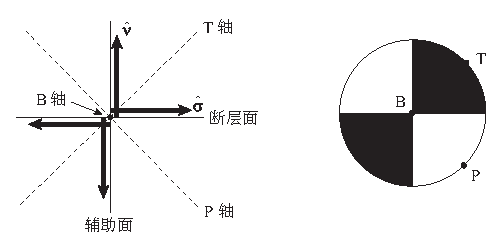
\includegraphics{../figures/chap05/fig07.eps}
\end{center}
\caption[beachball1]{\label{fig5.7}
({\em 左图\/}) 等价于一个右旋走滑断层的静态力
${\bf f}_{\rm f}=-M_0(\bnuh\bsigmah+
\bsigmah\bnuh)\cdot{\mbox{\boldmath $\nabla$}}\hspace{-0.2 mm}
\delta({\bf x}-{\bf x}_{\rm s})$ 的俯视图。
({\em 右图\/}) 其相应的沙滩球,其中标明了 T、B 和 P 轴,即
$\hat{\bf e}_+=(\bnuh+\bsigmah)/\sqrt{2}$、
$\hat{\bf e}_0=\bnuh\times\bsigmah$ 和
$\hat{\bf e}_-=(\bnuh-\bsigmah)/\sqrt{2}$ 的投影。这一双力偶源的中间轴,即
B~轴,位于两个正交的 P 波节面的交线上。值得注意的是,在这个例子中要区分东西走向的右旋滑动与南北走向的左旋滑动是不可能的,因为它们的点源 P 波辐射花样是一样的。
\index{nodal-plane ambiguity}%
}
\end{figure}

在全球地震学中,一个地震的矩张量习惯上用震中处的球极坐标分量来表示:
\eq \label{5.Mmatconv}
\bM=\left(\begin{array}{ccc}
M_{rr} & M_{r\theta} & M_{r\phi} \\
\vspace{-1.0 mm} & \vspace{-1.0 mm} & \vspace{-1.0 mm} \\
M_{\theta r} & M_{\theta\theta} & M_{\theta\phi} \\
\vspace{-1.0 mm} & \vspace{-1.0 mm} & \vspace{-1.0 mm} \\
M_{\phi r} & M_{\phi\theta} & M_{\phi\phi}
\end{array}\right),
\en
其中 $M_{r\theta}=M_{\theta r}$, $M_{r\phi}
=M_{\phi r}$ 和 $M_{\theta\phi}=M_{\phi\theta}$。
径向、余纬向和经向单位矢量分别指向上方、南方和东方。
对于图~\ref{fig5.7}中东西走向的右旋走滑断层,
$\hat{M}_{\theta\phi}=\hat{M}_{\phi\theta}=
-1/\!\sqrt{2}$ ,其它分量均为零。
表~5.1汇集了一些基本的双力偶与非双力偶震源机制的 $\hat{\bM}$ 及其震源球。

\begin{table}
\label{table5.1}
\centering
\begin{tabular}{|l|c||l|c|} \hline
     &     &     &      \\
\hspace{2.0 mm}矩张量 & 沙滩球
& \hspace{4.0 mm}矩张量 & 沙滩球 \\
     &     &     &      \\ \hline
     &     &     &      \\
\hspace{2.8 mm}$\frac{1}{\sqrt{3}}
\left(\begin{array}{rrr}
 1 &  0 &  0 \\
 0 &  1 &  0 \\
 0 &  0 &  1 \\
\end{array}\right)$
&
\begin{tabular}{l}
\vspace{0.25cm}
\rotatebox{270}{\scalebox{.0625}{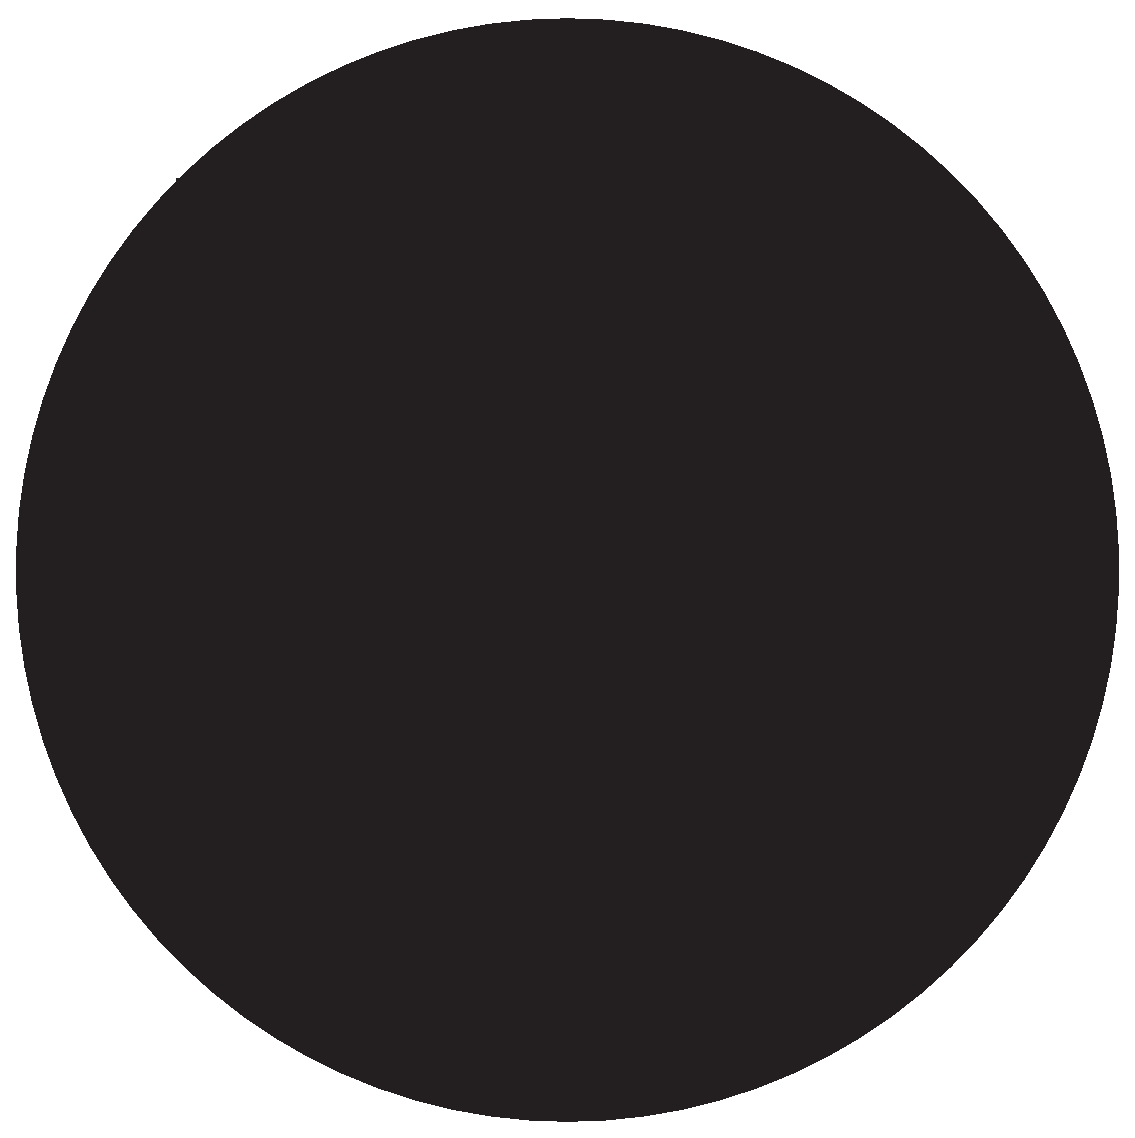
\includegraphics{../figures/beachballs/beachball7.eps}}}
\end{tabular}
&
$-\frac{1}{\sqrt{3}}
\left(\begin{array}{rrr}
 1 &  0 &  0 \\
 0 &  1 &  0 \\
 0 &  0 &  1 \\
\end{array}\right)$
&
\begin{tabular}{l}
\vspace{0.25cm}
\rotatebox{270}{\scalebox{.0625}{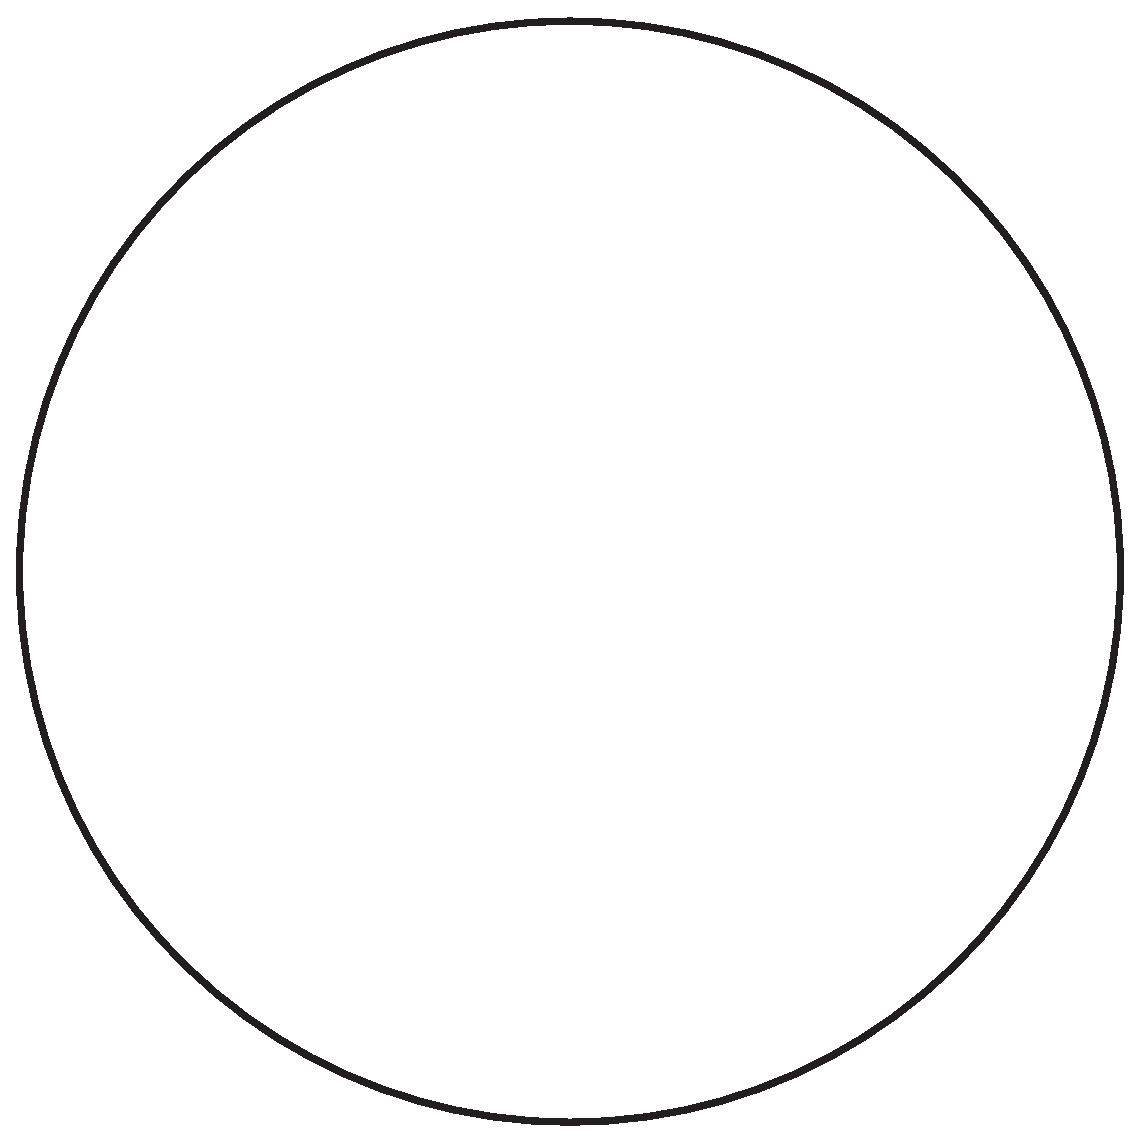
\includegraphics{../figures/beachballs/beachball8.eps}}}
\end{tabular}
\\
$-\frac{1}{\sqrt{2}}
\left(\begin{array}{rrr}
 0 &  0 &  0 \\
 0 &  0 &  1 \\
 0 &  1 &  0 \\
\end{array}\right)$
&
\begin{tabular}{l}
\vspace{0.25cm}
\rotatebox{270}{\scalebox{.0625}{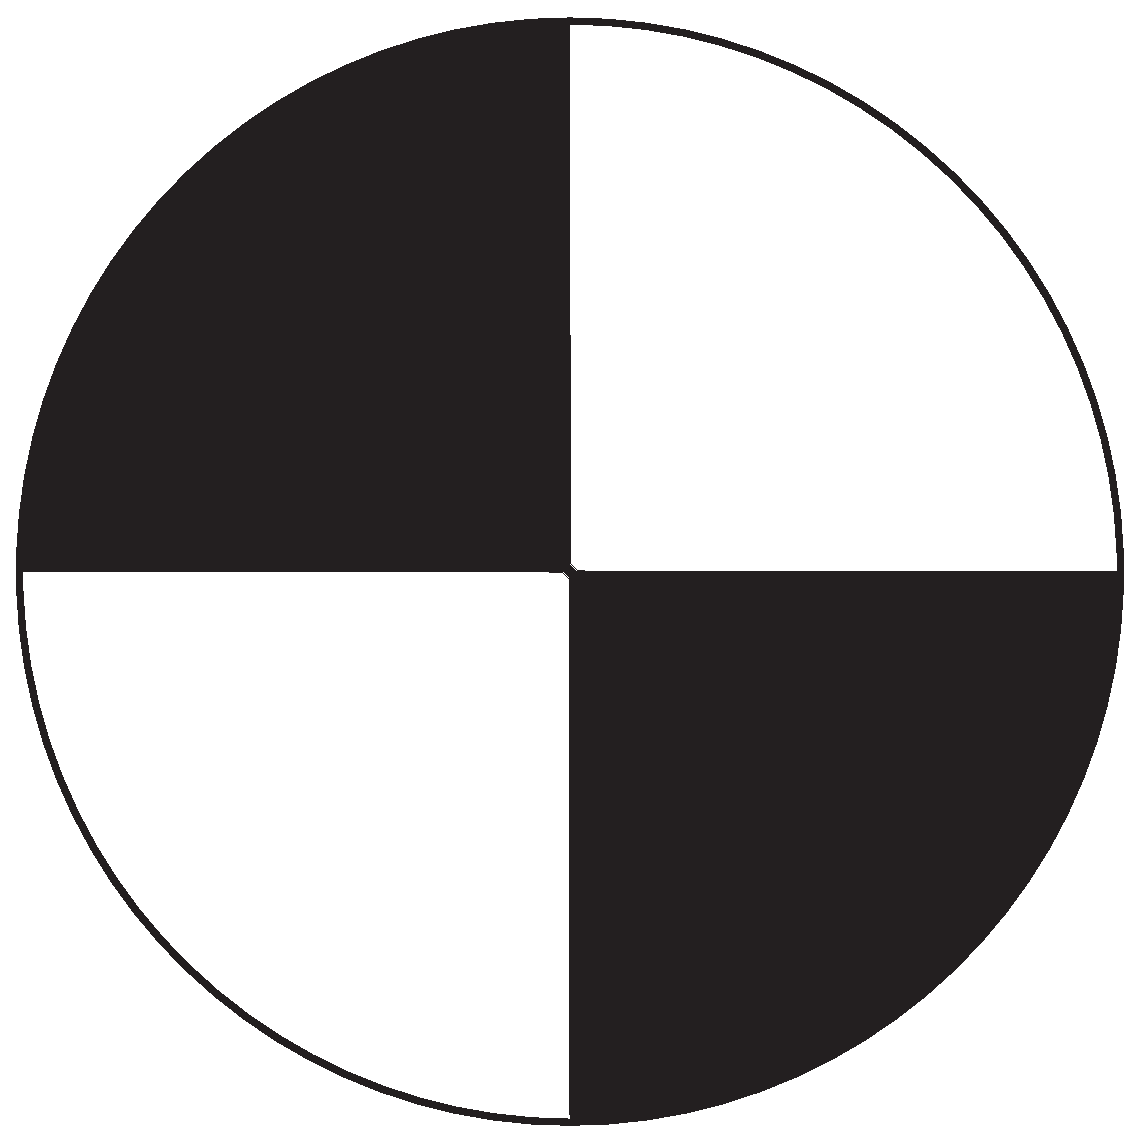
\includegraphics{../figures/beachballs/beachball6.eps}}}
\end{tabular}
&
\hspace{2.8 mm}$\frac{1}{\sqrt{2}}
\left(\begin{array}{rrr}
 0 &  0 &  \hspace{-1.0 mm}0 \\
 0 &  1 &  \hspace{-1.0 mm}0 \\
 0 &  0 & \hspace{-1.0 mm}-1 \\
\end{array}\right)$
&
\begin{tabular}{l}
\vspace{0.25cm}
\rotatebox{270}{\scalebox{.0625}{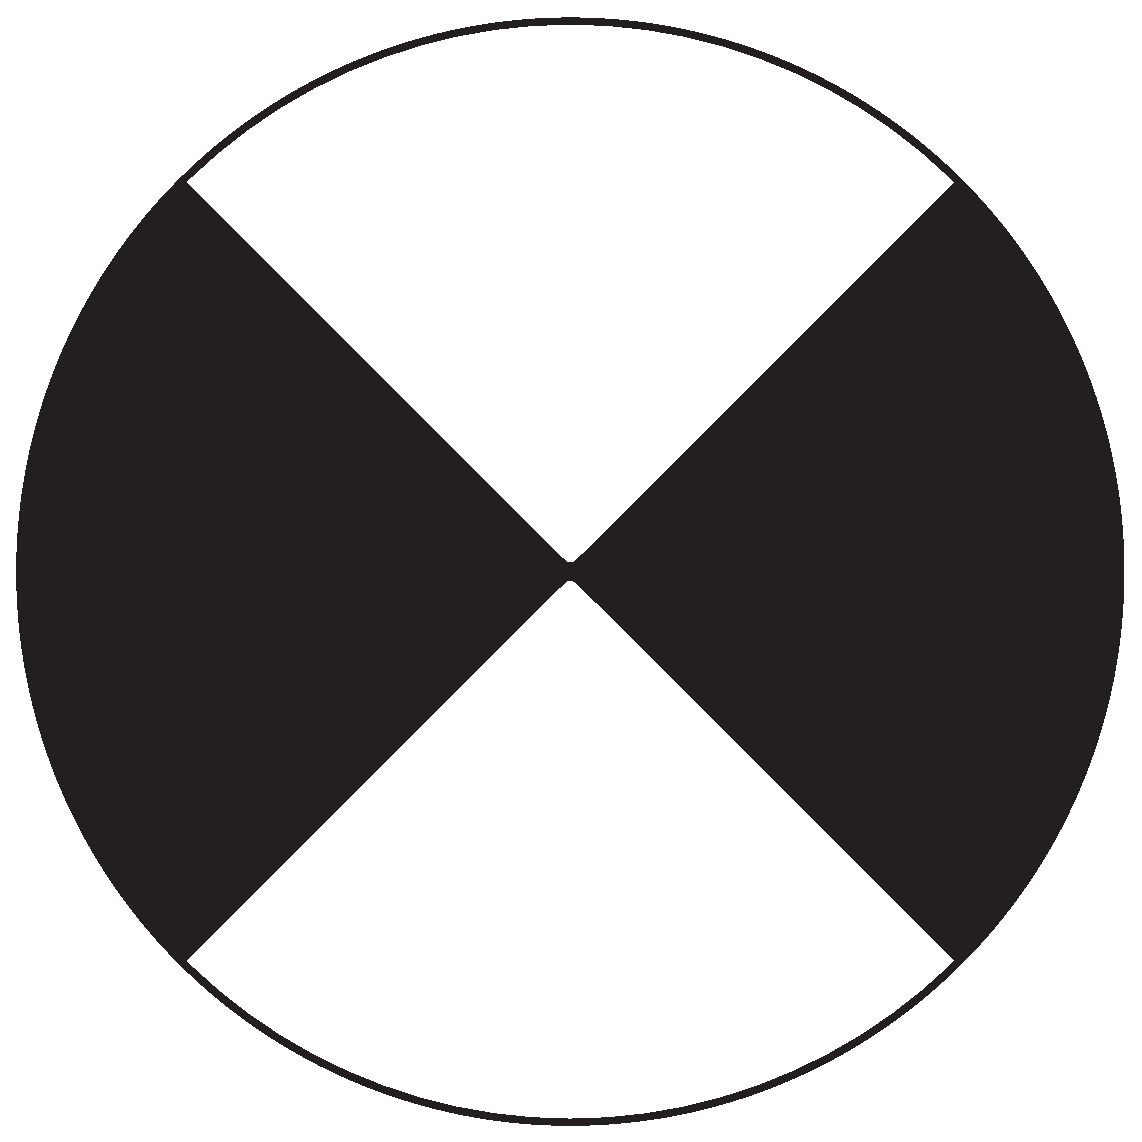
\includegraphics{../figures/beachballs/beachball2.eps}}}
\end{tabular}
\\
\hspace{2.8 mm}$\frac{1}{\sqrt{2}}
\left(\begin{array}{rrr}
 0 &  1 &  0 \\
 1 &  0 &  0 \\
 0 &  0 &  0 \\
\end{array}\right)$
&
\begin{tabular}{l}
\vspace{0.25cm}
\rotatebox{270}{\scalebox{.0625}{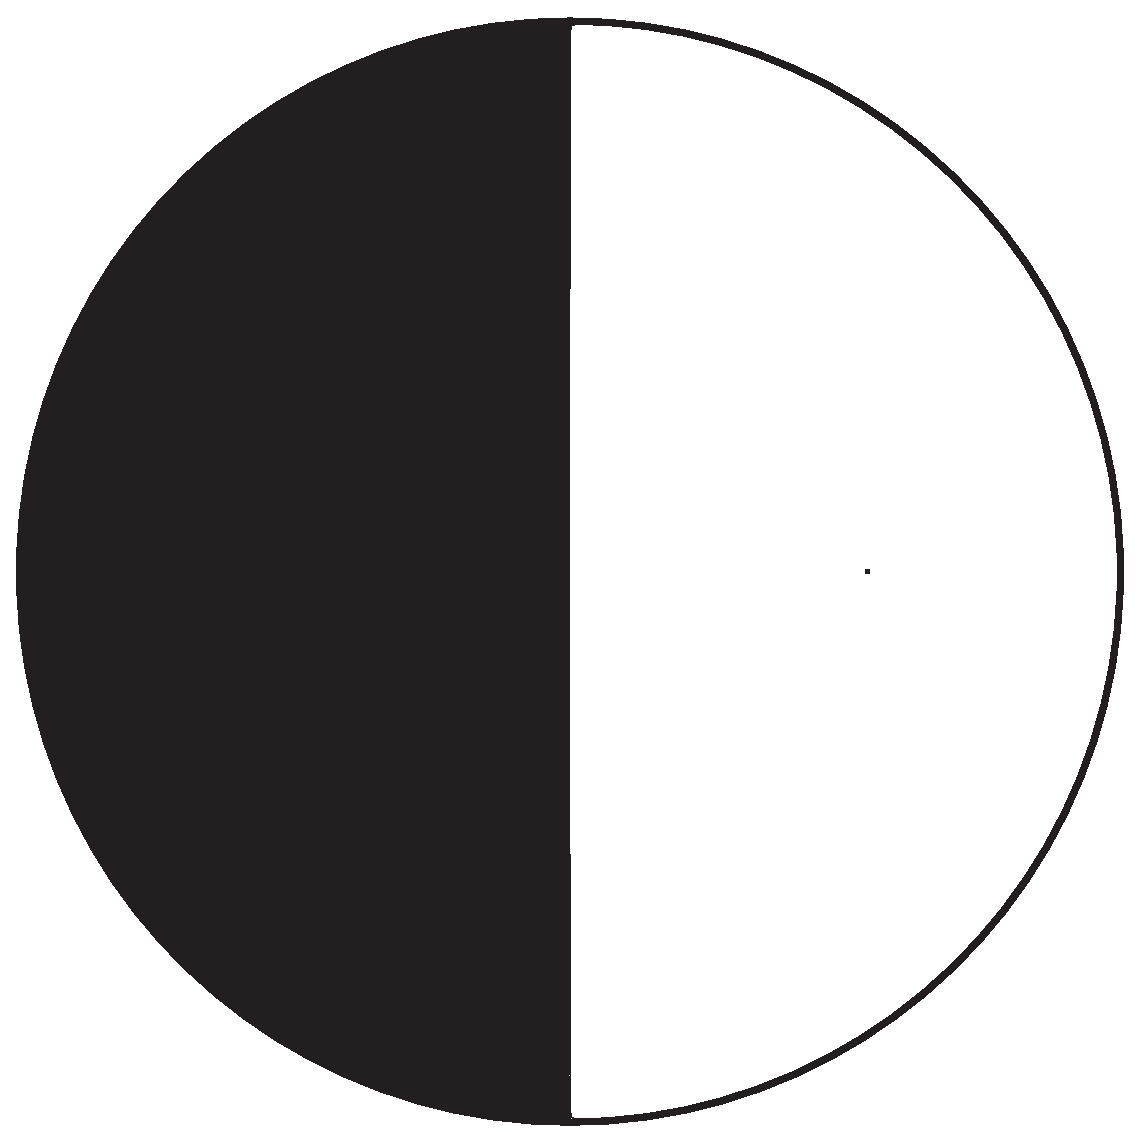
\includegraphics{../figures/beachballs/beachball4.eps}}}
\end{tabular}
&
\hspace{2.8 mm}$\frac{1}{\sqrt{2}}
\left(\begin{array}{rrr}
 0 &  0 &  1 \\
 0 &  0 &  0 \\
 1 &  0 &  0 \\
\end{array}\right)$
&
\begin{tabular}{l}
\vspace{0.25cm}
\rotatebox{270}{\scalebox{.0625}{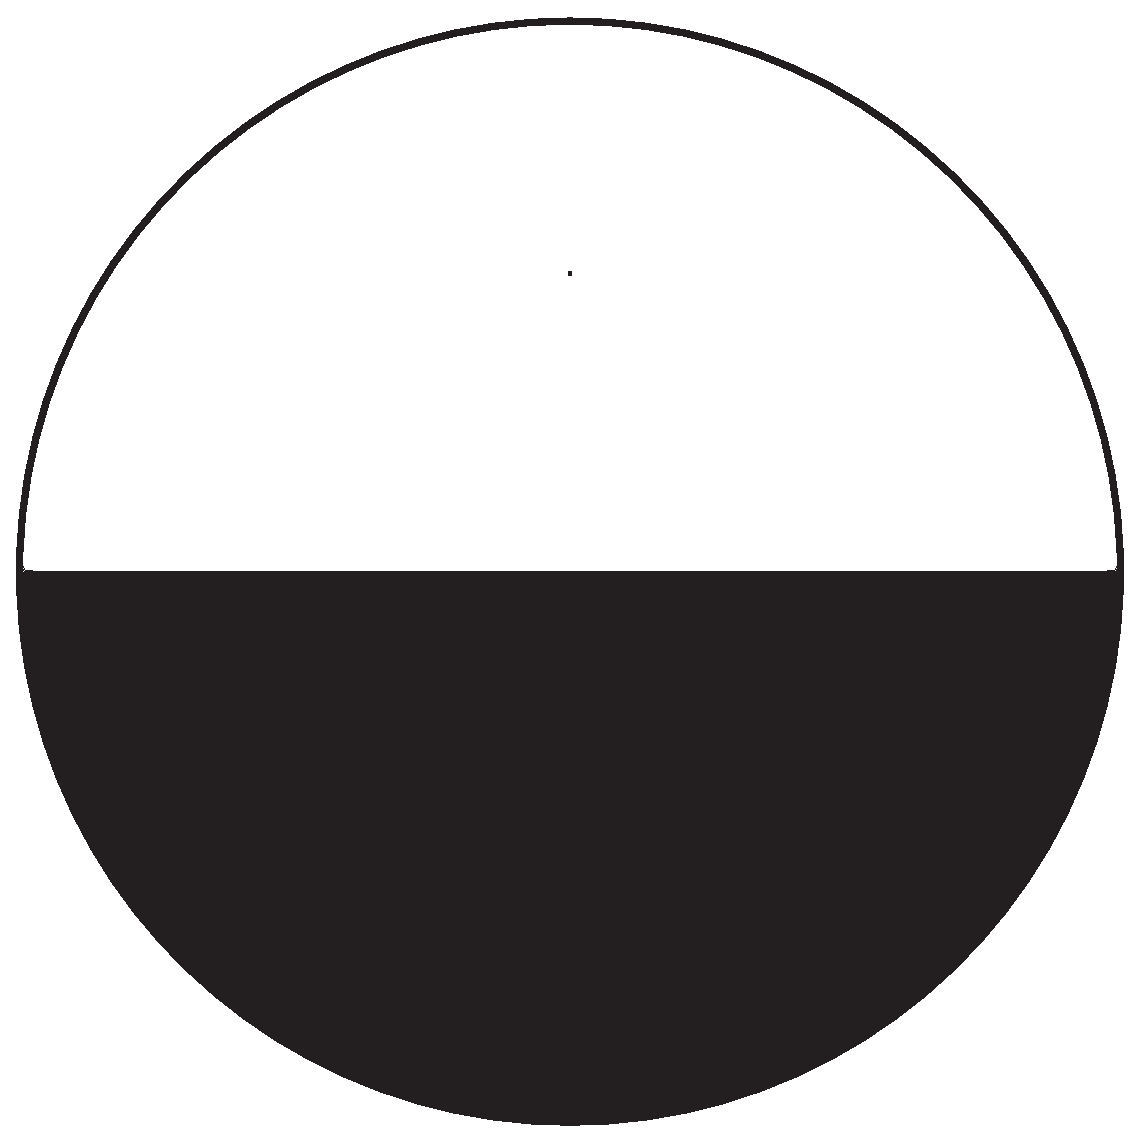
\includegraphics{../figures/beachballs/beachball5.eps}}}
\end{tabular}
\\
\hspace{2.8 mm}$\frac{1}{\sqrt{2}}
\left(\begin{array}{rrr}
 1 &  \hspace{-1.0 mm}0 &  0 \\
 0 & \hspace{-1.0 mm}-1 &  0 \\
 0 &  \hspace{-1.0 mm}0 &  0 \\
\end{array}\right)$
&
\begin{tabular}{l}
\vspace{0.25cm}
\rotatebox{270}{\scalebox{.0625}{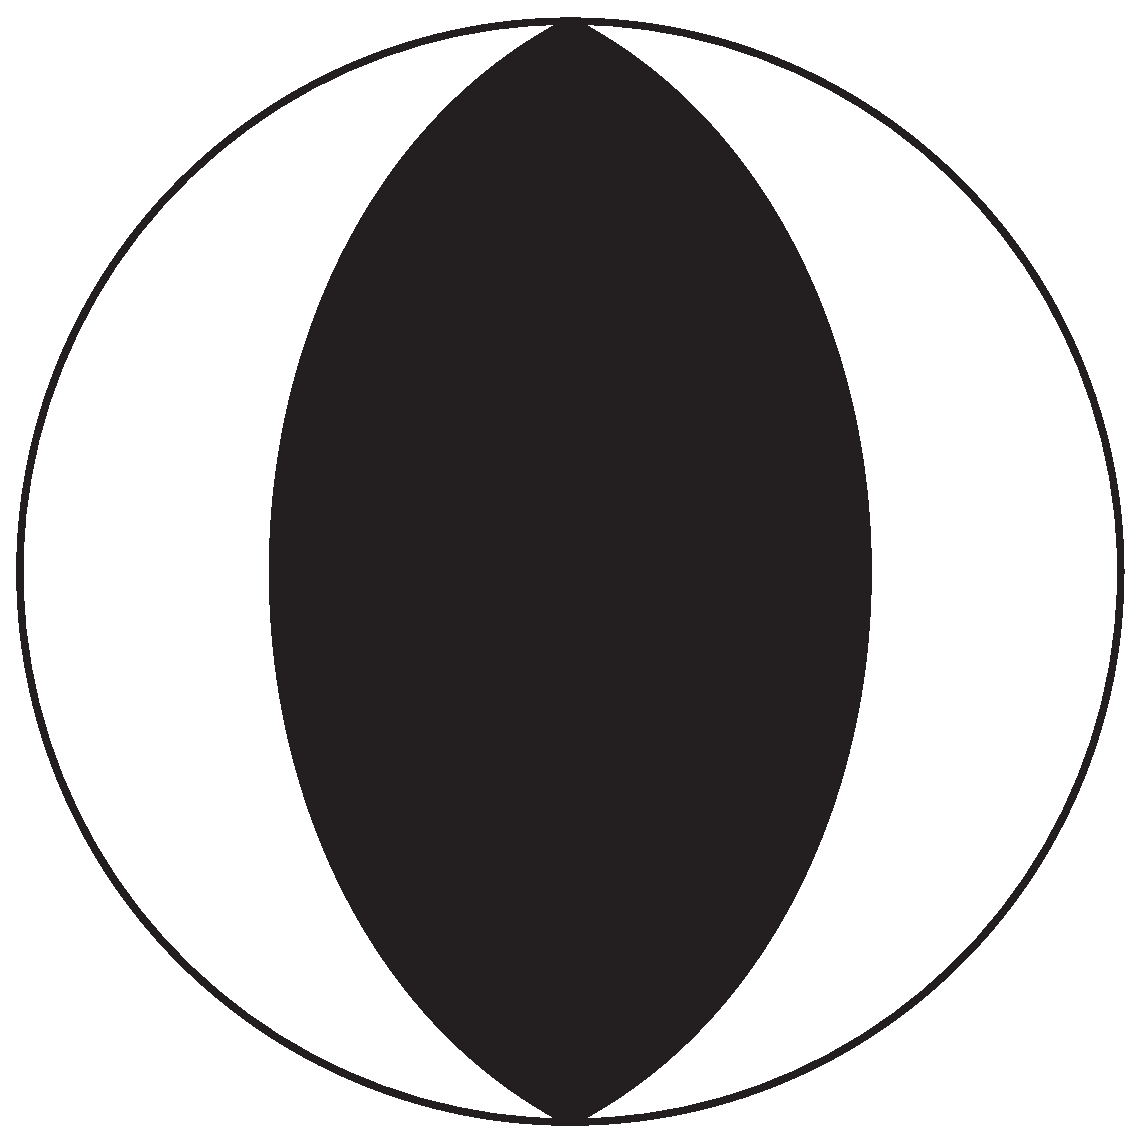
\includegraphics{../figures/beachballs/beachball1.eps}}}
\end{tabular}
&
\hspace{2.8 mm}$\frac{1}{\sqrt{2}}
\left(\begin{array}{rrr}
 1 &  0 &  \hspace{-1.0 mm}0 \\
 0 & 0 &  \hspace{-1.0 mm}0 \\
 0 &  0 &  \hspace{-1.0 mm}-1 \\
\end{array}\right)$
&
\begin{tabular}{l}
\vspace{0.25cm}
\rotatebox{270}{\scalebox{.0625}{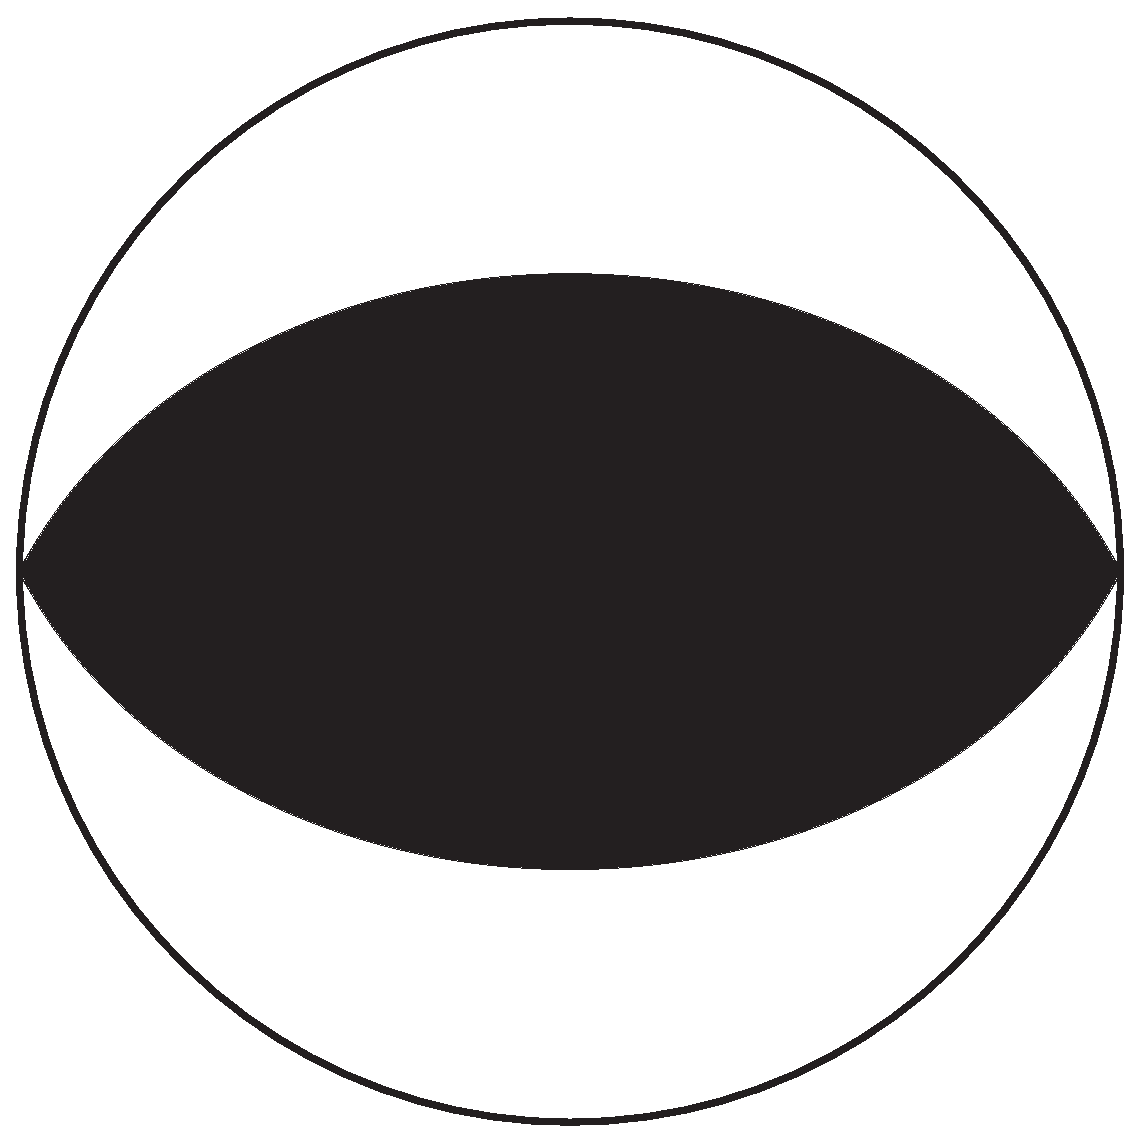
\includegraphics{../figures/beachballs/beachball3.eps}}}
\end{tabular}
\\
\hspace{2.8 mm}$\frac{1}{\sqrt{6}}
\left(\begin{array}{rrr}
 1 &  0 &  \hspace{-1.0 mm}0 \\
 0 &  1 &  \hspace{-1.0 mm}0 \\
 0 &  0 &  \hspace{-1.0 mm}-2 \\
\end{array}\right)$
&
\begin{tabular}{l}
\vspace{0.25cm}
\rotatebox{270}{\scalebox{.0625}{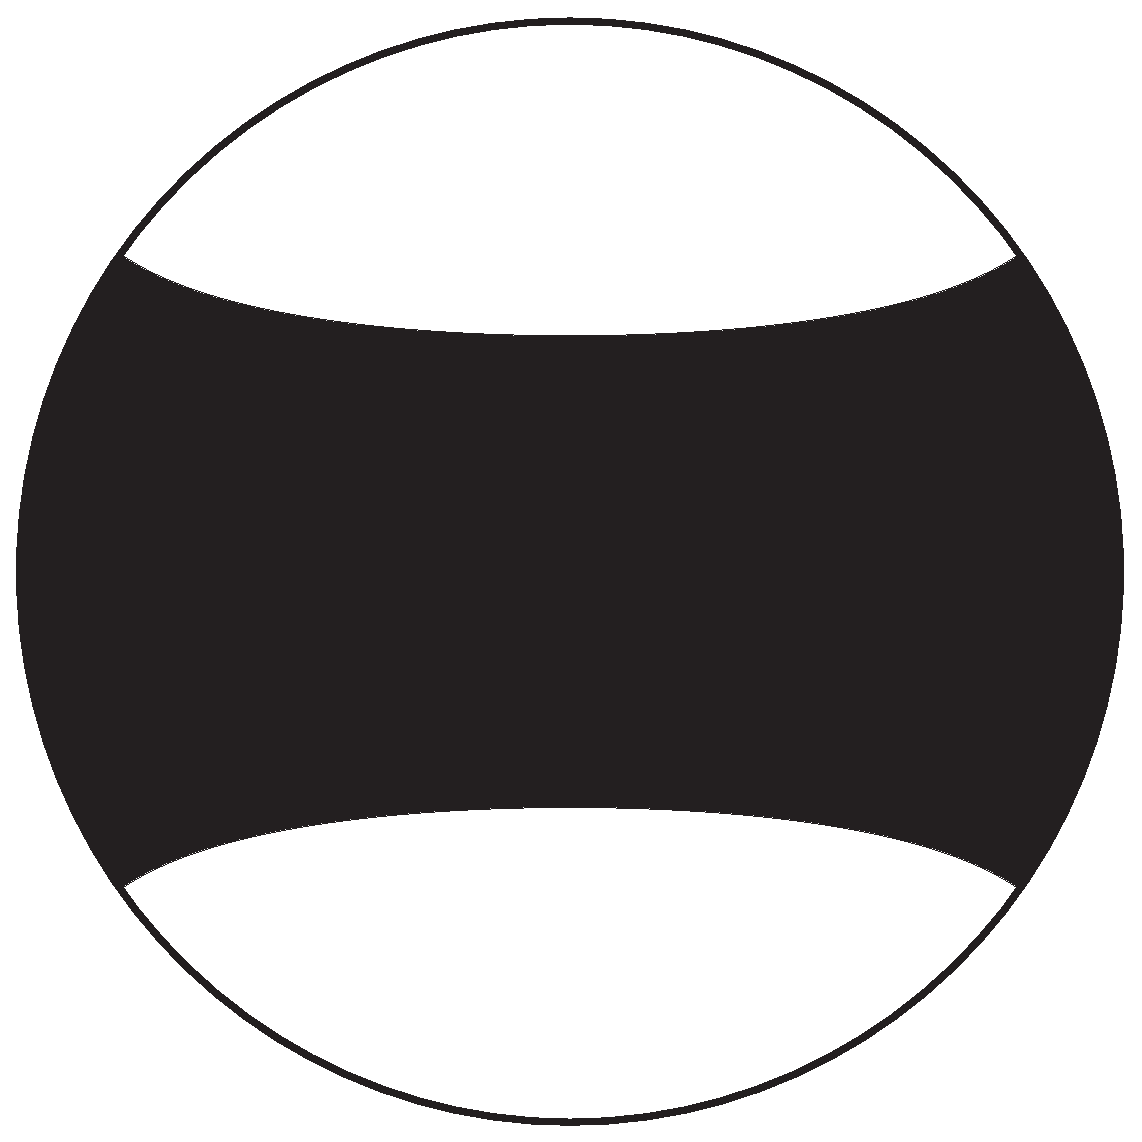
\includegraphics{../figures/beachballs/beachball9.eps}}}
\end{tabular}
&
\hspace{2.8 mm}$\frac{1}{\sqrt{6}}
\left(\begin{array}{rrr}
 1 &  \hspace{-1.0 mm}0 &  0 \\
 0 &  \hspace{-1.0 mm}-2 &  0 \\
 0 &  \hspace{-1.0 mm}0 &  1 \\
\end{array}\right)$
&
\begin{tabular}{l}
\vspace{0.25cm}
\rotatebox{270}{\scalebox{.0625}{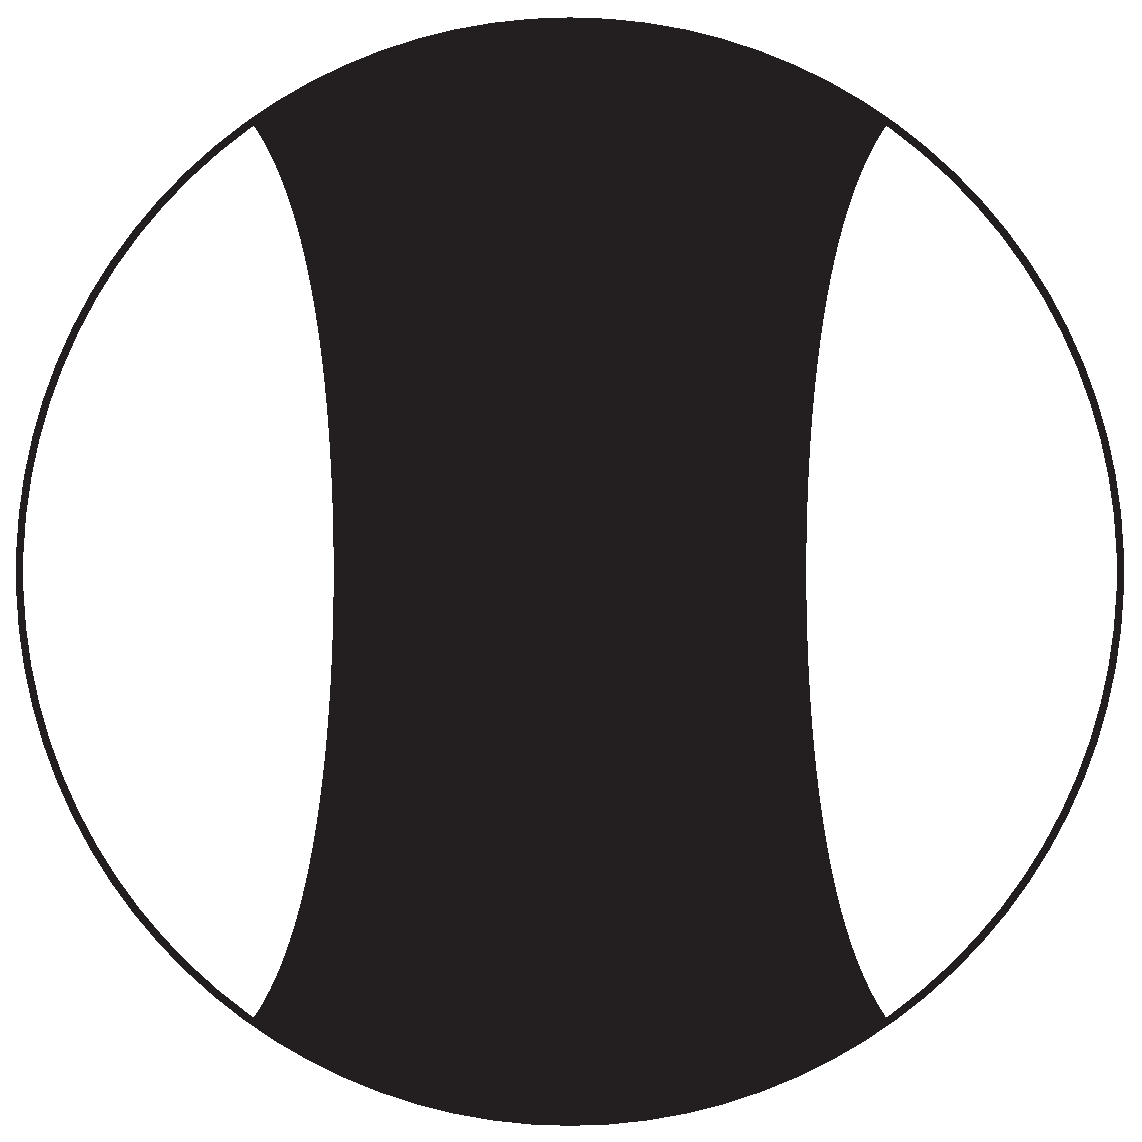
\includegraphics{../figures/beachballs/beachball10.eps}}}
\end{tabular}
\\
\hspace{2.8 mm}$\frac{1}{\sqrt{6}}
\left(\begin{array}{rrr}
 \hspace{-1.0 mm}-2 &  0 &  0 \\
 \hspace{-1.0 mm}0 &  1 &  0 \\
 \hspace{-1.0 mm}0 &  0 &  1 \\
\end{array}\right)$
&
\begin{tabular}{l}
\vspace{0.25cm}
\rotatebox{270}{\scalebox{.0625}{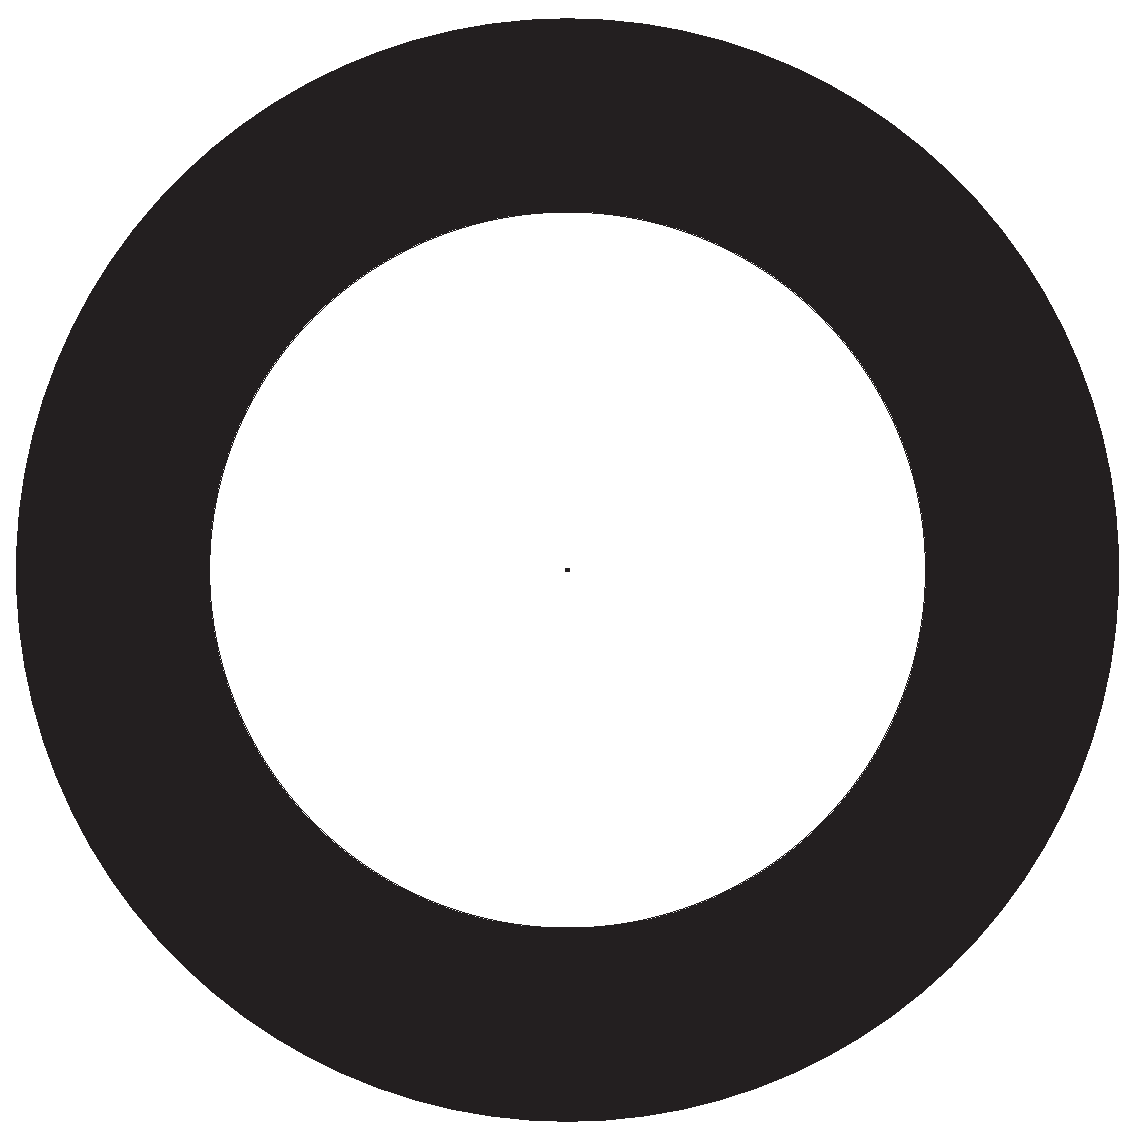
\includegraphics{../figures/beachballs/beachball11.eps}}}
\end{tabular}
&
$-\frac{1}{\sqrt{6}}
\left(\begin{array}{rrr}
 \hspace{-1.0 mm}-2 &  0 &  0 \\
 \hspace{-1.0 mm}0 &  1 &  0 \\
 \hspace{-1.0 mm}0 &  0 &  1 \\
\end{array}\right)$
&
\begin{tabular}{l}
\vspace{0.25cm}
\rotatebox{270}{\scalebox{.0625}{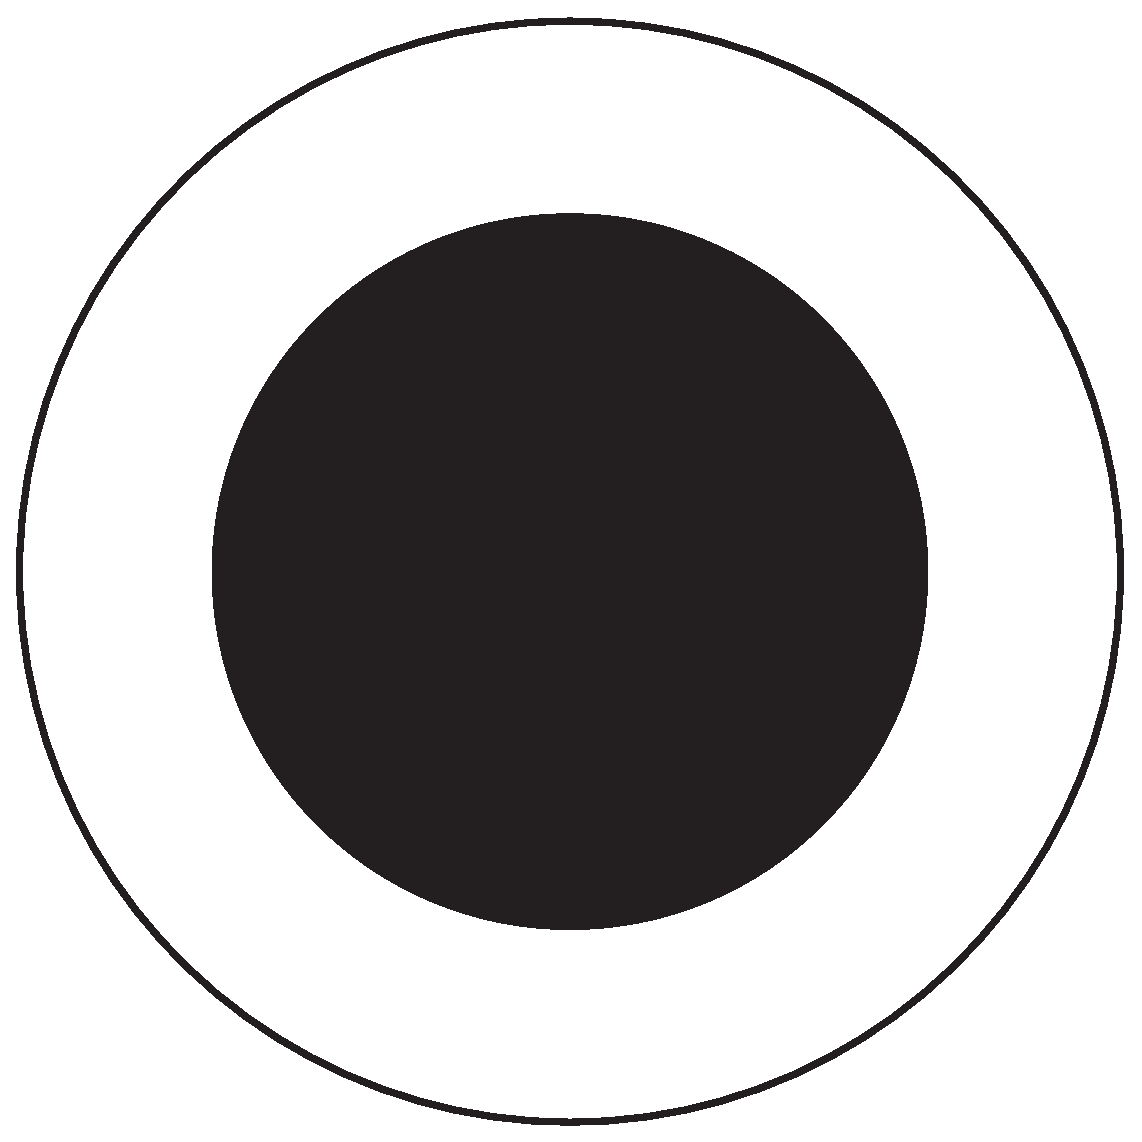
\includegraphics{../figures/beachballs/beachball12.eps}}}
\end{tabular}
\\
     &     &     &      \\ \hline
\end{tabular}
\caption[beachballs]{
一些基本的单位矩张量$\hat{\bf M}$及其相应的沙滩球。分量 
$\hat{M}_{rr},\hat{M}_{\theta\theta},\ldots,
\hat{M}_{\theta\phi}$ 以~(\ref{5.Mmatconv}) 中的约定排列。
最上一行中全黑的沙滩球是纯爆破源
$\hat{\bf M}={\bf I}/\hspace{-0.2 mm}\sqrt{3}$,另一个全白的沙滩球是纯内爆源
$\hat{\bf M}=-{\bf I}/\hspace{-0.2 mm}\sqrt{3}$。
接着的三行是一些双力偶源,包括垂直走滑断层 ({\em 从上数第二行\/}),垂直倾滑断层 ({\em 从上数第三行\/}) 和 $45^{\circ}$ 倾角的逆冲断层
({\em 从上数第四行\/})。
第五行和第六行为纯补偿线矢量偶极子,最下面一行是理想的“眼球”或“煎蛋”式机制,
与图~\ref{fig5.9}中的类似。除了外爆源和内爆源,其它所有震源都有纯偏矩张量:
${\rm tr}\,\hat{\bf M}=0$。
\index{linear vector dipole!compensated}%
\index{explosion}%
\index{implosion}%
\index{source!explosion}%
\index{source!implosion}%
\index{source!strike-slip}%
\index{source!thrust}%
\index{source!dip-slip}%
\index{source!eyeball}%
\index{source!fried-egg}%
\index{nodal-plane ambiguity}%
}
\end{table}

\begin{sidewaysfigure}
\centering
\rotatebox{270}
{
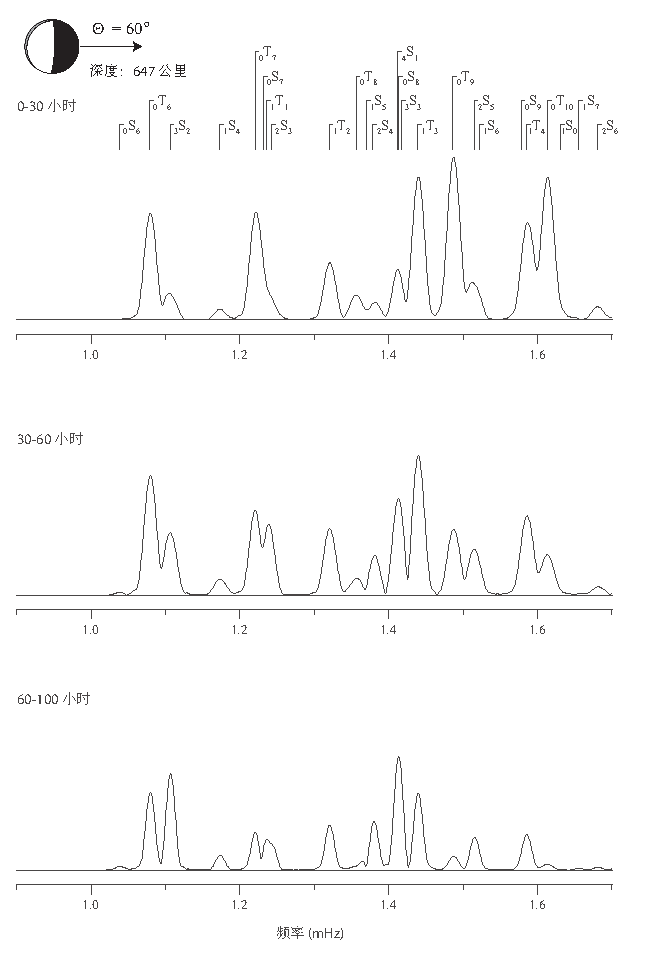
\includegraphics{../figures/chap05/fig08.eps}
}
\caption[global seismicity]{
哈佛大学矩心矩张量目录中发生在1976--1997年间,震源深度小于
~50~公里 的共10,219个地震的震中位置和震源机制。每个沙滩球的大小与地震矩
$M_0$ 的对数成正比。世界地图是以等面积圆柱投影所绘制,阴影部分为陆地。
(由 E.\ Larson提供。)
}
\label{fig5.8}
\end{sidewaysfigure}
哈佛大学矩心矩张量和其它震源机制目录中的大多数地震都属于浅源的板块边界地震,而这些地震的最佳拟合双力偶的断层面与辅助面较容易分辨。图~\ref{fig5.8}中的俯视图显示这些地震一贯地以走滑机制在转换断层带上发生以及以低角度逆冲机制沿削减带发生,这一现象是板块构造的最引人注目的表现之一。
\begin{figure}[!b]
\begin{center}
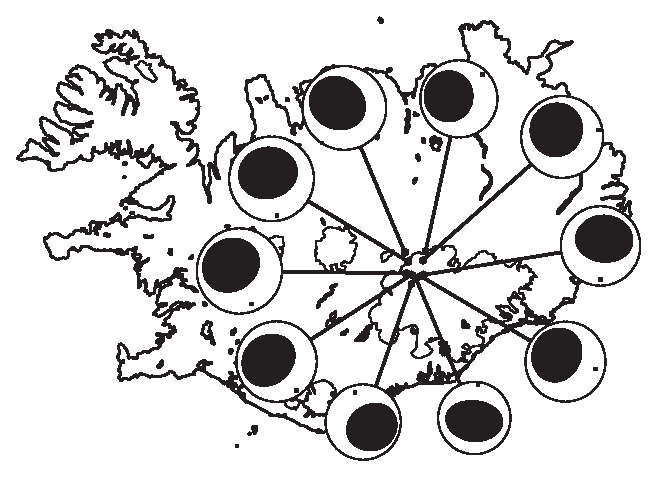
\includegraphics{../figures/chap05/fig09.eps}
\end{center}
\caption[iceland]{
\label{fig5.9}
哈佛大学矩心矩张量目录中震中({\em 每一条与震源球连线的端点\/})位于冰岛冰川下的B\'{a}rdarbunga火山附近的10个地震(1976--1996)的震源机制。所有这些貌似“眼球”或“煎蛋”的事件均为近乎纯补偿线矢量偶极子,其 T 轴近乎垂直,表明同时受到垂直向伸张和水平向压缩的作用。每个“眼球”里的“小黑点”是P轴。
(由 M.\ Nettles 和 G.\ Ekstr\"{o}m 提供。)
}
\end{figure}
这些地震的滑动矢量的切向分量为描述当今板块运动的欧拉矢量提供了重要约束
(Minster \& Jordan
\citeyear{minster&jordan78}; De Mets, Gordon, Argus
\& Stein \citeyear{demets&al90})。
图~\ref{fig5.9} 显示了位于冰岛B\'{a}rdarbunga火山附近的一组非比寻常却又很有意思的非双力偶型地震,
\index{non-double couple}%
\index{source!non-double-couple}%
它们的“眼球”或“煎蛋”式的震源机制在一些其它火山地区也已经被发现。
\index{source!fried-egg}%
\index{source!eyeball}%
这些地震被认为是环绕火山口、向外倾斜的弯曲断层在深部岩浆库膨胀作用下发生滑动的结果
(Ekstr\"{o}m
\citeyear{ekstrom94})。
\index{beachball|)}%

\subsection{震源时间函数}
\index{source time function|(}%

在频率较高时,特别是在远震体波的分析中,有必要考虑震源的有限特性。在最简单的近似下,我们忽略震源的矩心偏移 $\bDelta\bx$ 及其在空间上的有限范围;而其时间上的有限过程则通过将
~(\ref{5.deltaglut})中的脉冲型的应力过剩率拓展为:
\eq
\label{5.generglut}
\p_t\bS=\dot{\bM}(t)\,\delta(\bx-\bx_{\rm s}).
\en
来模拟。$\dot{M}(t)$ 为
{\em 矩率张量\/},即瞬时应力过剩率的体积分:
\index{tensor!moment-rate}%
\index{moment-rate tensor}%
\eq
\dot{\bM}(t)=\int_{S^t}\p_t\bS\,dV.
\en
这一具有时间依赖性的点源的简正模式响应~(\ref{5.accresp})为
\eq
\label{5.Mwresp}
\ba(\bx,t)=\Re{\rm e}\sum_k\bM(\omega_k)
\!:\!\beps^*_k(\bx_{\rm s})_{\,}\bs_k(\bx)
\exp\,i\omega_k(t-t_{\rm s}),
\en
其中
\eq \label{5.Momofom}
\bM(\omega)=\exp(i\om t_{\rm s})\int_{t_0}^{t_{\rm f}}
\dot{\bM}(t)\exp(-i\omega t)\,dt.
\en
(\ref{5.Mwresp}) 式与对狄拉克函数形式的应力过剩的响应~(\ref{5.Mresp})完全一样, 只是把 $\bM$ 换成~(\ref{5.Momofom})中的
{\em 依赖频率的矩张量\/}。
\index{moment tensor!frequency-dependent}%
值得注意的是 $\bM(\om)$ 并不是依赖时间的矩张量 $\bM(t)$的傅里叶变换; 而是时移因子 $\exp(i\om t_{\rm s})$ 与矩率张量 $\dot{\bM}(t)$ 的傅里叶变换的乘积。

在使用~(\ref{5.Mwresp}) 时通常假定震源是{\em 同步的\/},
\index{source!synchronous}%
\index{synchronous source}%
意思是 $\dot{\bM}(t)$ 的所有分量对时间的依赖是相同的。为方便起见,这种同步源可以写成如下形式
\eq \label{5.syncsrc}
\dot{\bM}(t)=\sqrt{2}M_0\hat{\bM}_{\,}\dot{m}(t),
\en
其中 $M_0$ 和 $\hat{\bM}$ 分别为依赖时间的标量矩和~(\ref{5.moment2})--(\ref{5.unitmom})中定义的单位矩张量。$\dot{m}(t)$ 是归一化的{\em 震源时间函数\/},它满足 
\index{source time function!normalized}%
\index{normalized source time function}%
\eq
\int_{t_0}^{t_{\rm f}}\dot{m}(t)\,dt=1.
\en
在这一近似下,~(\ref{5.littlem})中的归一化应力过剩率密度为
$\dot{m}(\bx,t)=\dot{m}(t)_{\,}\delta(\bx-\bx_{\rm s})$。
在无初始偏应力的流体静力学地球中,具有单向滑动的平面断层肯定是同步的;其震源时间函数是滑动速率的加权平均:
\eq
\dot{m}(t)=\frac{1}{M_0}\int_{\Sigma^t}\mu\hspace{0.2 mm}\p_t\Delta s\,d\/\Sigma.
\en
在远震体波波形观测分析中,大地震的震源时间函数
$\dot{m}(t)$ 一般表示为一系列的矩形时窗或者是有重叠的梯形或等腰三角形时窗
(Langston \citeyear{langston81};
Kikuchi \& Kanamori \citeyear{kikuchi&kanamori82};
N\'{a}b\v{e}lek \citeyear{nabelek85};
 Ekstr\"{o}m \citeyear{ekstrom89})。

一个同步点源的频率依赖矩张量为
$\bM(\omega)=\sqrt{2}M_0\hat{\bM}_{\,}m(\omega)$,
其中
\eq \label{5.mofom}
m(\omega)=\exp(i\om t_{\rm s})\int_{t_0}^{t_{\rm f}}\dot{m}(t)\exp(-i\omega t)\,dt.
\en
在 $\omega\rightarrow 0$ 的低频极限,~(\ref{5.mofom}) 中的变换可以近似为截断的泰勒展开:
\eq \label{5.mofom2}
m(\omega)=1-i\omega(\Delta t)-
\half\om^2(\Delta t)^2-\sixth\omega^2\tau_{\rm h}^2,
\en
其中
\eq
\Delta t=t_{\rm c}-t_{\rm s}=\int_{t_0}^{t_{\rm f}}
(t-t_{\rm s})\dot{m}(t)\,dt,
\en
\eq \label{5.taudef}
\tau_{\rm h}^2=3\int_{t_0}^{t_{\rm f}}(t-t_{\rm c})^2\dot{m}(t)\,dt.
\en
这里的 $\Delta t$ 是 $\dot{m}(t)$ 的时间矩心 $t_{\rm c}$ 相对于震源参照时间
$t_{\rm s}$ 的偏移,如图~\ref{fig5.10}所示,而 $\tau_{\rm h}$ 是对震源在时间上的{\em 半宽度\/}的一个估计。
\index{half-duration}%
\index{source half-duration}%
定义式~(\ref{5.taudef}) 中的系数3使得当震源时间函数为矩形时窗时,即
\eq
\dot{m}(t)
=(t_{\rm f}-t_0)^{-1}[H(t-t_0)-H(t-t_{\rm f})],
\en
$\tau_{\rm h}$ 恰好等于 $\half(t_{\rm f}-t_0)$。
哈佛大学矩心矩张量解的常规处理中使用的就是这样的以
$t_{\rm c}=\half(t_0+t_{\rm f})$
为中心,名义上半宽度为
$\tau_{\rm h}=2.4\times 10^{-6}M_0
^{\raise-0.7ex\hbox{$\scriptstyle 1/3$}}$ 的矩形时窗,其中
$\tau_{\rm h}$ 和 $M_0$ 的单位分别为秒和牛顿 米 (G.\ Ekstr\"{o}m,
私人通讯, 1996)。
\begin{figure}
\begin{center}
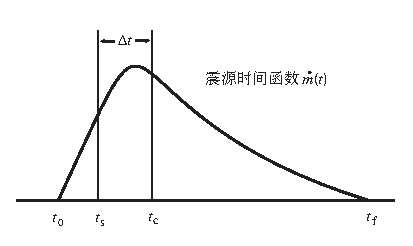
\includegraphics{../figures/chap05/fig10.eps}
\end{center}
\caption[sourcetime]{\label{fig5.10}
一个起始于 $t_0$ 终止于 $t_{\rm f}$ 的地震震源时间函数 $\dot{m}(t)$ 示意图。矩心时间 \vspace{-0.3 mm}
$t_{\rm c}=
\int_{t_0}^{t_{\rm f}}t\,\dot{m}(t)\,dt$ 相对于震源参照时间 $t_{\rm s}$ 的偏移量为 $\Delta t$。}
\end{figure}
Silver \& Jordan (\citeyear{silver&jordan82}; \citeyear{silver&jordan83})
和 Ihml\'{e} \& Jordan (\citeyear{ihmle&jordan94}; \citeyear{ihmle&jordan95})
使用了类似于 (\ref{5.mofom2}) 的展开式来分析所谓的“慢”地震,他们将
$\tau_{\rm h}$ 用一个“特征”震源持续时间 $\tau_{\rm c}=(4/3)^{1/2}
\hspace{0.2 mm}\tau_{\rm h}$ 来替代。

一个自洽的震源表述在考虑震源的有限特性时应该在空间和时间坐标上具有同样的量级。由于这个原因,在解释用上述推导所得到的对震源持续时间“半宽度”的估计时需要格外谨慎;实际上, $\tau_{\rm h}$ 虽只是表观半宽度,但它同时反映了地震破裂的空间和时间的尺度。
Backus (\citeyear{backus77a}; \citeyear{backus77b}) 将应力过剩率张量
$\p_t\bS$ 做多项式矩展开到二阶,并且展示了如何将得到的时-空矩与震源的持续时间、空间尺度和方向性联系起来。但是,在这种一般的二阶矩分析中需要确定的参数个数十分惊人。为了把参数数目减少到较为可控,\textcite{bukchin94}考虑了一种{\em 空间延伸同步源\/},其形式为
\index{source!spatial}%
\index{source!synchronous}%
\index{synchronous source}%
$\p_t\bS=\sqrt{2}M_0\hat{\bM}_{\,}\dot{m}(\bx,t)$。描述这种震源除了矩张量 $\bM=\sqrt{2}M_0\hat{\bM}$ 以外,只需要其归一化标量应力过剩率密度
$\dot{m}(\bx,t)$ 中的四个一阶矩和十个二阶矩。

为简单起见,在本书后续章节中我们将忽略地震震源的空间和时间矩心偏移
$\bDelta\bx$ 和 $\Delta t$ 及其空间延伸。此外,我们还将设定震源参照时间为零时刻:
\eq \label{5.newconv}
t_{\rm s}=0.
\en
一般来说,我们将使用应力过剩率为 $\p_t\bS=\bM\,\delta(\bx-\bx_{\rm s})
\,\delta(t)$ 的脉冲矩张量源,其相关的等效力密度为 
$\bef=-\bM\cdot\bdel\delta(\bx-\bx_{\rm s})\,H(t)$。
我们将把对这种震源的响应写成~(\ref{5.Mdispl})--(\ref{5.Mresp})的形式,
并按~(\ref{5.newconv})的约定设 $t_{\rm s}$ 为零。在任何质点加速度 $\ba(\bx,t)$ 或 $\ba(\bx,\om)$ 的模式叠加表达式中,可以很容易地通过
$\bM\rightarrow\bM(\om_k)=
\int_{t_0}^{t_{\rm f}}\dot{\bM}(t)\exp(-i\om_kt)\,dt$ 这一变换来考虑有限持续时间的震源,这里
$\dot{\bM}(t)$ 是依赖于时间的矩率张量,$\om_k$ 是所考虑的本征频率。
在第12章和第15章中讨论弹性和非弹性地球中的体波传播时,我们将考虑依赖时间的矩率张量为
$\dot{\bM}(t)=\sqrt{2}M_0\hat{\bM}\,\dot{m}(t)$ 的同步震源。
\index{source time function|)}%

\renewcommand{\thesubsection}{$\!\!\!\raise1.3ex\hbox{$\star$}\!\!$
\arabic{chapter}.\arabic{section}.\arabic{subsection}}
\subsection{疑难震源}
\index{source!problematical|(}
\renewcommand{\thesubsection}{\arabic{chapter}.\arabic{section}.\arabic{subsection}}

在两种情形下点源矩张量表述会导致地震震源机制确定的困难;一个是震源位于固态自由表面或海底附近,另一个是震源跨越一个固-固不连续面 $\Sigma_{\rm SS}$。在本节中我们简短地讨论这两种疑难情况,并将把注意力集中在各向同性且具有流体静力学初始应力的地球模型。

我们已经看到,在自转地球模型中对矩张量源的响应与标量积
$\bM\!:\!\bepsilon^*$ 成正比,而这里为简单起见,我们已略去应变本征函数  $\bepsilon_k$ 上指定模式的角标k。在固态自由表面的动力学边界条件
$\bnh\cdot\bT^{\rm L1}=\bzero$ 意味着
\eq
\label{5.Mnear}
\varepsilon_{xz}=\varepsilon_{yz}=0,
\en
\eq
\label{5.Mnear2}
(\kappa+\fourthirds\mu)\varepsilon_{zz}
+(\kappa-\twothirds\mu)(\varepsilon_{xx}+\varepsilon_{yy})=0,
\en
其中我们采用了 $\bzh$ 轴垂直于边界的局地笛卡尔坐标系。由于剪切应变条件~(\ref{5.Mnear}) 当震源位置 $\bx_{\rm s}$ 接近固态自由表面或海底时,$M_{xz}$ 和 $M_{yz}$ 对 $\bM\!:\!\bepsilon^*$ 的贡献为零。
因此,对于浅源地震,矩张量 $\bM$ 中的这些垂向倾滑分量无法很好地约束。同样地,条件~(\ref{5.Mnear2}) 意味着任何满足如下关系的近地表震源
\eq
M_{zz}=\left(\frac{\kappa+\fourthirds\mu}
{\kappa-\twothirds\mu}\right)M_{xx}
=\left(\frac{\kappa+\fourthirds\mu}
{\kappa-\twothirds\mu}\right)M_{yy}.
\en
对激发振幅 $\bM\!:\!\bepsilon^*$ 的贡献都可以忽略不计。后面这个涉及对角元素
$M_{zz}$ 和 $M_{xx}+M_{yy}$ 之间互相依赖的问题可以通过采用
~(\ref{5.notrace}) 的矩张量迹为零的约束,即 $M_{xx}+M_{yy}+M_{zz}=0$ 来解决。但是,对非对角元素 $M_{xz}$ 和 $M_{yz}$ 则没有简易的解决办法。一个常用却显然是随意性的做法是干脆在确定浅源地震震源机制时将 $M_{xz}$ 和 $M_{yz}$ 均设为零;
Ekstr\"{o}m \& Dziewonski (\citeyear{ekstrom&dziewonski85})
证明这一做法对剩下的约束较佳的分量 $M_{xy}$,$M_{xx}-M_{yy}$
和 $M_{zz}=-M_{xx}-M_{yy}$ 几乎没有影响。这种疑难地震的一种尤其明显的例子是浅部近水平向的滑坡事件,如伴随1980年圣海伦斯火山爆发而产生的滑坡。观测与理论研究都已经表明,这种震源也可以用地表的水平点力来描述 (Kanamori \& Given
\citeyear{kanamori&given82}; Okal \citeyear{okal90};
Dahlen \citeyear{dahlen93})。

接下来我们假定最终的震源区被界面 $\Sigma_{\rm SS}$ 的一部份分为两个区域,即 $S^{\rm f}=S^+\cup S^-$, 且跨过该界面弹性模量 $\kappa$ 和 $\mu$ 是不连续的,如图~\ref{fig5.11}所示。
\begin{figure}[!b]
\begin{center}
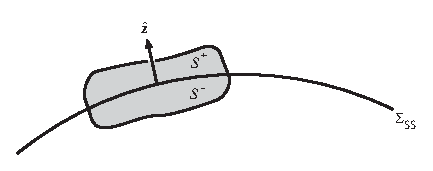
\includegraphics{../figures/chap05/fig11.eps}
\end{center}
\caption[sourcespan]{\label{fig5.11}
震源体积 $S^{\rm f}=S^+\cup S^-$ 跨越一个固-固不连续面
 $\Sigma_{\rm SS}$ 的示意图。如往常的定义一样,局地单位法向矢量
$\hat{\bf z}$ 指向不连续面的 $+$ 侧。}
\end{figure}
\textcite{woodhouse81a}已经考虑了这种跨越固-固不连续面的震源,我们在此只简述他的结论。在这种情形下,把标量积 $\bM\!:\!\bepsilon^*$ 用
$\bM^+\!:\!\bepsilon^{+*}+\bM^-\!:\!\bepsilon^{-*}$ 替代,
其中 $\bepsilon^{\pm}$ 是在边界 $\Sigma_{\rm SS}$两侧的应变, $\bM^{\pm}$ 为其相应的部分矩张量
\eq
\label{5.parmom}
\bM^{\pm}=\int_{S^{\pm}}\bS_{\rm f}\,dV.
\en
位移本征函数的连续性 $[\bs]^+_-=\bzero$ 确保了切向应变是连续的
\eq
\label{5.Mspan}
[\varepsilon_{xx}]^+_-=[\varepsilon_{yy}]^+_-=[\varepsilon_{xy}]^+_-,
\en
同时,牵引力的连续性
$[\bnh\cdot\bT^{\rm L1}]^+_-=\bzero$ 则确保
\eq
\label{5.Mspan2}
[\mu\varepsilon_{xz}]^+_-=[\mu\varepsilon_{yz}]^+_-=0,
\en
\eq
\label{5.Mspan3}
[(\kappa+\fourthirds\mu)\varepsilon_{zz}+
(\kappa-\twothirds\mu)(\varepsilon_{xx}+\varepsilon_{yy})]^+_-=0,
\en
这里我们又一次采用了 $\bzh$ 轴垂直于边界的局地笛卡尔坐标系。
利用~(\ref{5.Mspan})--(\ref{5.Mspan3}) 的条件,我们可以将激发振幅仅用不连续面两侧的其中一侧上的应变
$\bepsilon^+$ 或 $\bepsilon^-$ 来表示:
\eq
\label{5.plusmin}
\bM^+\!:\!\bepsilon^{+*}+\bM^-\!:\!\bepsilon^{-*}=
\bsM^+\!:\!\bepsilon^{+*}=\bsM^-\!:\!\bepsilon^{-*}.
\en
在~(\ref{5.plusmin})的两个表达示中的 $\bsM^+$ 和 $\bsM^-$ 可以显式公式给定
\eq
\sM_{xx}^{\pm}=M_{xx}^++M_{xx}^-+a_{\pm}M_{zz}^{\mp},
\en
\eq
\sM_{yy}^{\pm}=M_{yy}^++M_{yy}^-+a_{\pm}M_{zz}^{\mp},
\en
\eq
\sM_{zz}^{\pm}=M_{zz}^{\pm}+b_{\pm}M_{zz}^{\mp},
\en
\eq
\sM_{xz}^{\pm}=M_{xz}^{\pm}+c_{\pm}M_{xz}^{\mp},
\en
\eq
\sM_{yz}^{\pm}=M_{yz}^{\pm}+c_{\pm}M_{yz}^{\mp},
\en
\eq
\sM_{xy}^{\pm}=M_{xy}^++M_{xy}^-,
\en
其中
\eq
a_{\pm}=\frac{(\kappa_{\pm}-\twothirds\mu_{\pm})
-(\kappa_{\mp}-\twothirds\mu_{\mp})}
{\kappa_{\mp}+\fourthirds\mu_{\mp}},
\en
\eq
b_{\pm}=\frac{\kappa_{\pm}+\fourthirds\mu_{\pm}}
{\kappa_{\mp}+\fourthirds\mu_{\mp}}, \qquad
c_{\pm}=\frac{\mu_{\pm}}{\mu_{\mp}}.
\en
显然,实际震源等价于一个 $\Sigma_{\rm SS}$ 的 $+$ 侧上的矩张量源 $\bsM^+$,或者是一个 $\Sigma_{\rm SS}$ 的 $-$ 侧上的矩张量源 $\bsM^-$。
两个视矩张量 $\bsM^+$ 和 $\bsM^-$ 分别为假定地震发生在 $\Sigma_{\rm SS}$ 的 $+$ 侧或 $-$ 侧上,然后反演地震数据所得到的震源机制解。两者均不代表真正的矩张量,真正的矩张量是
\eq
\bM=\bM^++\bM^-.
\en
事实上,如果对震源不在物理上做进一步假定的话,真实的矩张量是无法确定的。
一种可能的假定是 $\bM^+$ 和 $\bM^-$ 有相同的方向,即
\eq
\label{5.Mprop}
\bM^+=\gamma\bM,\qquad\bM^-=(1-\gamma)\bM,
\en
其中 $0\leq\gamma\leq 1$ 是一个表示震源位于不连续面的 $+$ 侧的比例的参数。满足~(\ref{5.Mprop}) 的一个震源的例子是跨越不连续面的单向滑动平面断层。采用这一假设,真实的矩张量 $\bM$ 可以很容易地用 $\bsM^+$ 或 $\bsM^-$ 二者之一确定;但是,结果会依赖于比例参数 $\gamma$。一般而言,由于没有足够的信息来独立设定这一参数,因此通常简单地假定 $\gamma=0$ 或 $\gamma=1$,即假定震源全部在不连续面的某一侧。

上面讨论的两种疑难情形从本质上讲都与震源的等效力表述无关;它们都是点源近似的结果。对于一个与固态自由表面或海底相交,或者跨越不连续面 $\Sigma_{\rm SS}$ 的有限震源,其等效体力密度 $\bef$ 和表面牵引力 $\bt$ 都是有严格定义的。唯一在根本上有问题的震源是与 $\Sigma_{\rm SS}$ 的一部份有{\em 重叠\/}的理想断层,对此 $\bef$ 和 $\bt$ 是无法定义的。
\index{source!problematical|)}
\index{source!point|)}%
\index{point source|)}%

\renewcommand{\thesection}{$\!\!\!\raise1.3ex\hbox{$\star$}\!\!$
\arabic{chapter}.\arabic{section}}
\section{地震的能量平衡}
\index{earthquake energy balance|(}%
\index{energy balance|(}%
\label{5.sec.energy}
\renewcommand{\thesection}{\arabic{chapter}.\arabic{section}}

在本章的结尾,我们讨论一下地震破裂中的能量平衡。为简单起见,我们仅考虑{\em 无自转\/}地球的情况;而由于自转而造成的复杂性仅在第5.5.4节简短提及。

\renewcommand{\thesubsection}{$\!\!\!\raise1.3ex\hbox{$\star$}\!\!$
\arabic{chapter}.\arabic{section}.\arabic{subsection}}
\subsection{净能量释放}
\index{energy release|(}%
\label{5.sec.release}
\renewcommand{\thesubsection}{\arabic{chapter}.\arabic{section}.\arabic{subsection}}

由于地震是自发现象,因此地震必须通过做功使得在破裂发生之前地球中所储存的能量能够被释放出来。释放的总能量与破裂在时间历程上的细节无关;而只依赖于破裂终止且所有自由振荡的简正模式都衰减完毕之后的地球最终的静态平衡状态。我们取地震发生之前的初始平衡状态为弹性和引力势能的零点或参照点;
\index{static equilibrium}%
\index{equilibrium!static}%
则本质上为正的{\em 能量释放\/} $\sE_{\rm r}$
\index{released energy}%
\index{energy!released}%
是最终状态的静态弹性-引力能的 {\em 负号\/}:
\eq
\label{5.DeltaE}
\sE_{\rm r}=-\sE_{\rm e}-\sE_{\rm g},
\en
其中
\eq
\label{5.Estatelas}
\sE_{\rm e}=
\int_{\subearth}[\bT^0\!:\!\beps_{\rm f}
+\half\bdel\bs_{\rm f}
\!:\!\bLambda\!:\!\bdel\bs_{\rm f}]\,dV,
\en
\eq
\label{5.Estatgrav}
\sE_{\rm g}=
\int_{\subearth}\rho^0[\bs_{\rm f}
\cdot\bdel\phi^0
+\half\bs_{\rm f}\cdot\bdel
\phi^{\rm E1}_{\rm f}
+\half\bs_{\rm f}
\cdot\bdel\bdel\phi^0
\cdot\bs_{\rm f}]\,dV.
\en
(\ref{5.Estatgrav})式中的 $\phi^{\rm E1}_{\rm f}$ 是最终的静态欧拉引力势函数微扰。

在~(\ref{5.DeltaE})--(\ref{5.Estatgrav})中使用高斯定理,并考虑不连续性 $\bDelta\bs_{\rm f}=[\bs_{\rm f}]^+_-$,我们可以将 $\sE_{\rm r}$ 写为在最终的断层面 $\Sigma^{\rm f}$ 上的积分。如同第3.9.4节的做法,我们利用固-液不连续 $\Sigma_{\rm FS}$ 面上的二阶切向滑动条件 $[\bnh\cdot\bs_{\rm f}-\bs_{\rm f}\cdot\bdel^{\Sigma}
(\bnh\cdot\bs_{\rm f})+\half\bs_{\rm f}\cdot
(\bdel^{\Sigma}\bnh)\cdot\bs_{\rm f}]^+_-=0$,我们得到
\eqa
\label{5.manyints}
\lefteqn{\sE_{\rm r}=\int_{\subearth}\bs_{\rm f}
\cdot[\bdel\cdot\bT^0-\rho^0 \bdel\phi^0]\,dV} \nonumber \\
&&\mbox{}+\half\int_{\subearth}\bs_{\rm f}\cdot[\bdel\cdot
\bT^{\rm PK1}_{\rm f}-\rho^0\bdel\phi^{\rm E1}_{\rm f}-\rho^0\bs_{\rm f}
\cdot\bdel\bdel\phi^0]\,dV \nonumber \\
&&\mbox{}\quad-\half\int_{\spar\subearth}[\bnh\cdot(2\bT^0+
\bT^{\rm PK1}_{\rm f})\cdot\bs_{\rm f}]\,d\/\Sigma
\nonumber \\
&&\mbox{}\quad\quad+\half\int_{\Sigma_{\rm SS}}[\bnh\cdot(2\bT^0+
\bT^{\rm PK1}_{\rm f})\cdot\bs_{\rm f}]^+_-\,d\/\Sigma
\nonumber \\
&&\mbox{}\quad\quad\quad+\half\int_{\Sigma_{\rm FS}}[(2\bnh\cdot\bT^0+
\bt^{\rm PK1}_{\rm f})\cdot\bs_{\rm f}]^+_-\,d\/\Sigma
\nonumber \\
&&\mbox{}\quad\quad\quad\quad+\half\int_{\Sigma^{\rm f}}[\bnuh\cdot(2\bT^0+
\bT^{\rm PK1}_{\rm f})\cdot\bs_{\rm f}]^+_-\,d\/\Sigma,
\ena
其中
$\bT^{\rm PK1}_{\rm f}=\bLambda\!:\!\bdel\bs_{\rm f}$,$\bt^{\rm PK1}_{\rm f}=\bnh\cdot\bT^{\rm PK1}_{\rm f}
+\bnh\,\bdel^{\Sigma}\cdot(\varpi^0\bs_{\rm f})
-\varpi^0(\bdel^{\Sigma}\bs_{\rm f})\cdot\bnh$。
由于初始和终止地球模型中分别具有的静态弹性-重力平衡条件为 
\index{static equilibrium}%
\index{equilibrium!static}%
$\bdel\cdot\bT^0-\rho^0\bdel\phi^0=\bzero$ 和
$\bdel\cdot\bT^{\rm PK1}_{\rm f}-\rho^0
\bdel\phi^{\rm E1}_{\rm f}-\rho^0\bs_{\rm f}
\cdot\bdel\bdel\phi^0=\bzero$,因此~(\ref{5.manyints}) 中的两个体积分为零。
此外,因为初始牵引力的连续性条件 $[\bnh\cdot\bT^0]^+_-=\bzero$,再加上相应的静态位移所满足的边界条件,即在 $\p\earth$ 上 $\bnh\cdot\bT^{\rm PK1}_{\rm f}=\bzero$、在 $\Sigma_{\rm SS}$ 上 $[\bnh\cdot\bT^{\rm PK1}_{\rm f}]^+_-=
\bzero$、以及在 $\Sigma_{\rm FS}$ 上
$[\bt^{\rm PK1}_{\rm f}]^+_-=
\bnh[\bnh\cdot\bt^{\rm PK1}_{\rm f}]^+_-=\bzero$,故在自由表面和内部不连续面上的面积分也为零。
因而一个理想断层所释放的总弹性-重力能简化为
\eq
\label{5.DeltaE2}
\sE_{\rm r}=\half\int_{\Sigma^{\rm f}}[\bnuh\cdot(2\bT^0+\bT^{\rm
PK1}_{\rm f})\cdot\bs_{\rm f}]^+_-\,d\/\Sigma.
\en
矢量 $\half\bnuh\cdot(2\bT^0+\bT^{\rm PK1}_{\rm f})$ 是作用在断层面 $\Sigma^{\rm f}$ 任意一侧上的初始和最终牵引力的平均。

(\ref{5.DeltaE2}) 式与\textcite{reid10}在对1906年旧金山大地震的著名的调查报告中首次使用的理想断层能量释放的经典表达式非常相似。但通常在该结果的推导中会忽略自重力,同时假定初始静态应力是由相对于某种自然的无应变、无应力状态的无穷小初始应变所造成的 (Steketee \citeyear{steketee58};
Savage \citeyear{savage69}),然而这一假定与现实并不相符。现今的处理则更为合理,除了对地球的重力有所考虑,也对地球初始应力 $\bT^0$ 的大小或来源不做任何假设。人们已经熟知,
$\sE_{\rm r}$ 对 $\bT^0$ 的显性依赖使得对地震能量释放的测量不可能仅通过地震学的方法来实现。
\index{energy release|)}%

\renewcommand{\thesubsection}{$\!\!\!\raise1.3ex\hbox{$\star$}\!\!$
\arabic{chapter}.\arabic{section}.\arabic{subsection}}
\subsection{释放能量的耗散}
\renewcommand{\thesubsection}{\arabic{chapter}.\arabic{section}.\arabic{subsection}}

一个地震所释放的所有能量的最终命运都是在地球体积
$\earth$ 内部的某个地方被耗散掉。能量的耗散可以分为三个区域。首先,在破裂过程 $t_0\leq t\leq t_{\rm f}$ 中,在瞬时断层面 $\Sigma^t$ 两侧 壁上,由于要克服阻碍滑动的摩擦牵引力做功,能量会以热的形式耗散掉。
\index{work}%
其次,在这一时段中,在断层的瞬时扩张边缘即破裂前缘 $\p\Sigma^t_{\rm c}$, 由于要克服物质间的内聚力以生成新的断层面,或者有额外的生热,也会导致能量耗散。
\index{energy dissipation}%
\index{dissipation}%
最后,剩余的释放能量必须是地震所激发的地球简正模式振荡的能量;这些能量会在整个地球内部因无穷小的非弹性作用造成振荡衰减而被耗散掉。
体耗散在破裂起始的 $t=t_0$ 时刻发生,一直持续到所有模式的振荡全部衰减完毕。
我们现在来检视一下释放的能量 $\sE_{\rm r}$ 在这三种耗散机制中是如何分配的。

地球的动能加上弹性-重力势能随时间的瞬时变化率为
\eq
\label{5.Edot}
\dot{\sE}=\dot{\sE}_{\rm k}+\dot{\sE}_{\rm e}+\dot{\sE}_{\rm g},
\en
其中
\eq
\label{5.Ekdot}
\dot{\sE}_{\rm k}=\frac{d}{dt}
\int_{\subearth}[\half\rho^0\p_t\bs\cdot\p_t\bs]\,dV,
\en
\eq
\dot{\sE}_{\rm e}=\frac{d}{dt}
\int_{\subearth}[\bT^0\!:\!\beps+\half
\bdel\bs\!:\!\bLambda\!:\!\bdel\bs]\,dV,
\en
\eq
\label{5.Egdot}
\dot{\sE}_{\rm g}=\frac{d}{dt}\int_{\subearth}\rho^0[\bs
\cdot\bdel\phi^0 +\half\bs\cdot\bdel\phi^{\rm E1}
+\half\bs
\cdot\bdel\bdel\phi^0\cdot\bs]\,dV.
\en
要计算破裂发生的时间段 $t_0\leq t\leq t_{\rm f}$ 中的时间导数,我们必须特别关注传播中的破裂前缘
$\p\Sigma^t_{\rm c}$。
\index{rupture front}%
\index{crack tip}%
用 $\varepsilon$ 表示到这一弯曲前缘的距离。
\begin{figure}[!t]
\begin{center}
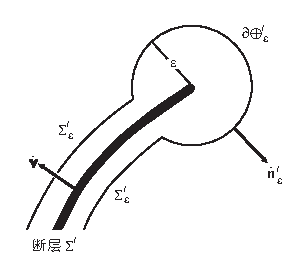
\includegraphics{../figures/chap05/fig12.eps}
\end{center}
\caption[cracktip]{\label{fig5.12}
一个传播中的破裂前缘附近的积分面的放大图。在半径不变的凸球面 $\partial\earth_{\varepsilon}^t$ 跟随破裂前缘移动时,紧贴断层 $\Sigma^t$ 两侧壁上的“薄饼” $\Sigma_{\varepsilon}^t$ 
会逐渐扩展。}
\end{figure}
物质内聚力或破裂前缘生热不为零的宏观表现为在 $\p_t\bs$ 和 $\bdel\bs$ 中具有
$\varepsilon^{-1/2}$ 奇异性,只要如我们所假定的,胡克定律只有在断层面
$\Sigma^t$ 上完全失效。为处理这些奇异性,我们把~(\ref{5.Ekdot})--(\ref{5.Egdot}) 中的体积分都看作是在一个包围断层面 $\Sigma^t$ 的有裂缝的体积内的积分极限,因而只剩下包围 $\p\Sigma^t_{\rm c}$ 的凸球面内的体积。用 $\p\earth_{\varepsilon}^t$ 表示该凸球的表面,
$\bnh_{\varepsilon}^t$ 为其向外的单位法向矢量,$\Sigma_{\varepsilon}^t$ 为断层面刚好在 $\Sigma^t$ 内部的部份,因而包覆断层的表面包含
$\p\earth_{\varepsilon}^t$ 以及 $\Sigma_{\varepsilon}^t$ 的两侧,如图~\ref{fig5.12} 所示。我们假定凸球面随
$\p\Sigma^t_{\rm c}$ 一起移动,并且其半径 $\varepsilon$ 不随时间变化;因而表面
$\p\earth^t_{\varepsilon}$ 相对于周围物质的向内的法向速度为
$-\bnh^t_{\varepsilon}\cdot\bv$,其中 $\bv$ 是破裂前缘的速度,即 {\em 破裂速度\/}。
\index{rupture velocity}%
\index{velocity!rupture}%
利用对移动体积上的积分求导的标准法则,以及高斯定理,我们可以把总能量的变化率
$\dot{\sE}$ 表示为
\eqa
\label{5.moreints}
\lefteqn{\dot{\sE}=\int_{\subearth}\p_t\bs
\cdot[\rho^0\bdel\phi^0-\bdel\cdot\bT^0]\,dV} \nonumber \\
&&\mbox{}+\int_{\subearth}\p_t\bs\cdot
[\rho^0\p_t^2\bs-\bdel\cdot
\bT^{\rm PK1}+\rho^0
\bdel\phi^{\rm E1}+\rho^0\bs
\cdot\bdel\bdel\phi^0]\,dV \nonumber \\
&&\mbox{}\quad+\int_{\spar\subearth}[\bnh\cdot(\bT^0+
\bT^{\rm PK1})\cdot\p_t\bs]\,d\/\Sigma
\nonumber \\
&&\mbox{}\quad\quad-\int_{\Sigma_{\rm SS}}[\bnh\cdot(\bT^0+
\bT^{\rm PK1})\cdot\p_t\bs]^+_-\,d\/\Sigma
\nonumber \\
&&\mbox{}\quad\quad\quad-\int_{\Sigma_{\rm FS}}[(\bnh\cdot\bT^0+
\bt^{\rm PK1})\cdot\p_t\bs]^+_-\,d\/\Sigma \nonumber\\
&&\mbox{}\quad\quad\quad\quad-\lim_{\varepsilon\rightarrow 0}
\int_{\Sigma^t_{\varepsilon}}[\bnuh\cdot(\bT^0+
\bT^{\rm PK1})\cdot\p_t\bs]^+_-\,d\/\Sigma \nonumber \\
&&\mbox{}\quad\quad\quad\quad\quad-\lim_{\varepsilon\rightarrow 0}
\int_{\spar\subearth_{\varepsilon}^t}
[e(\bnh_{\varepsilon}^t\cdot\bv)+\bnh_{\varepsilon}^t\cdot\bT^{\rm
PK1}\cdot\p_t\bs]\,d\/\Sigma, 
\ena
其中
$e=\half(\rho^0\p_t\bs\cdot\p_t\bs
+\bdel\bs\!:\!\bLambda\!:\!\bdel\bs)$。
在~(\ref{5.moreints}) 的推导中,我们使用了麦克斯韦关系
$\Lambda_{ijkl}=\Lambda_{klij}$、(\ref{4.gravid}) 中的对称关系和固-液边界 $\Sigma_{\rm FS}$ 上的二阶切向滑动条件~(\ref{3.slipsq3})。
根据静态平衡条件 $\rho^0\bdel\phi^0-\bdel\cdot\bT^0=\bzero$ 以及动量方程 
$\rho^0\p_t^2\bs-\bdel\cdot
\bT^{\rm PK1}+\rho^0
\bdel\phi^{\rm E1}+\rho^0\bs
\cdot\bdel\bdel\phi^0$=\bzero,
在 $\earth$ 上的体积分为零,
而初始牵引力连续性条件 $[\bnh\cdot\bT^0]^+_-=\bzero$ 以及~(\ref{3.Euler8})--(\ref{3.Euler9}) 中的边界条件又使得在
$\p\earth$、$\Sigma_{\rm SS}$ 和 $\Sigma_{\rm FS}$ 上的面积分也为零。
于是,~(\ref{5.moreints}) 式简化为
\eq
\label{5.Edot2}
\dot{\sE}=-\dot{\sE}_{\rm w}-\dot{\sE}_{\rm c},
\en
其中
\eq
\dot{\sE}_{\rm w}=\lim_{\varepsilon\rightarrow 0}
\int_{\Sigma^t_{\varepsilon}}[\bnuh\cdot(\bT^0+
\bT^{\rm PK1})\cdot\p_t\bs]^+_-\,d\/\Sigma,
\en
\eq
\label{5.Edotip}
\dot{\sE}_{\rm c}=\lim_{\varepsilon\rightarrow 0}
\int_{\spar\subearth_{\varepsilon}^t}
[e(\bnh_{\varepsilon}^t\cdot\bv)+\bnh_{\varepsilon}^t\cdot\bT^{\rm
PK1}\cdot\p_t\bs]\,d\/\Sigma.
\en
(\ref{5.Edot2}) 式右边第一项 $\dot{\sE}_{\rm w}$ 是在断层面 $\Sigma^t$ 两侧的 {\em 壁上\/}的瞬时摩擦能量耗散率,而第二项
$\dot{\sE}_{\rm c}$ 则代表了流入传播中的破裂前缘
$\p\Sigma^t_{\rm c}$ 的总能量通量。本质上两者都是正的,反映了破裂过程的不可逆性;
通量 $\dot{\sE}_{\rm c}$ 给出了在破裂前缘生成新的断层面所需要提供的能量速率的宏观估计。它包含两项的贡献,且各自都有简单的物理解释;第一项是因破裂前缘的运动而带来的平流贡献,第二项则是作用在 $\p\earth_{\varepsilon}^t$ 上的牵引力所做的功。另外还会有与 $\bnh^t_{\varepsilon}\cdot\bv$ 相乘的项存在,但是它们在
$\varepsilon\rightarrow 0$ 的极限下贡献为零,只要如我们所假定的,$\p_t\bs$
和 $\bdel\bs$ 的奇异性不会超过 $\varepsilon^{-1/2}$。

在断裂力学中,习惯上是估计破裂沿断层面 $\Sigma^t$ 前进时在{\em 单位距离\/}上而不是单位时间内能量流入破裂尖端的速率。由此得到的物理量---所谓的动力学{\em 能量释放率\/}---其定义为 $G=v^{-1}\dot{\sE}_{\rm c}$,
\index{energy release rate}%
其中 $v=\|\bv\|$ 为破裂速度。Freund (\citeyear{freund90}) 详尽地讨论了
$G$ 在力学上的重要性及其在建立动力学断裂条件中的角色。

\renewcommand{\thesubsection}{$\!\!\!\raise1.3ex\hbox{$\star$}\!\!$
\arabic{chapter}.\arabic{section}.\arabic{subsection}}
\subsection{地震能量}
\index{energy!seismic|(}%
\index{seismic energy|(}%
\renewcommand{\thesubsection}{\arabic{chapter}.\arabic{section}.\arabic{subsection}}

将~(\ref{5.Edot2}) 中的能量变化率在时间上从破裂起始时刻 $t=t_0$ 积分到 $t=\infty$,我们便可以得到前面提到的地震能量释放的三类分配的一个精确的清单。到目前为止,我们尚未明确引入造成地震之后振荡衰减的地球的非弹性。
现在我们假定它的唯一影响是在右边的求和 $-\dot{\sE}_{\rm w}-\dot{\sE}_{\rm c}$ 中加上一个无穷小的负数量,来代表整体耗散率。积分以后方程的左边是总能量变化,也就是静态能量释放的负数;能量平衡关系于是可以写成
\eq
\label{5.balance}
\sE_{\rm r}=\sE_{\rm s}
+\int_{t_0}^{t_{\rm f}}\dot{\sE}_{\rm w}\,dt
+\int_{t_0}^{t_{\rm f}}\dot{\sE}_{\rm c}\,dt,
\en
其中 $\sE_{\rm s}$ 是在 $t_0\leq t\leq\infty$ 时段上因整体非弹性而造成的总的能量耗散。
$\sE_{\rm s}$ 通常被称为{\em 地震能量\/}。
\index{seismic energy}%
\index{energy!seismic}%

在断层壁上的能量耗散率可以改写成如下形式
\eqa
\label{5.dEwall2}
\lefteqn{\dot{\sE}_{\rm w}=\frac{d}{dt}\left(
\lim_{\varepsilon\rightarrow 0}
\int_{\Sigma^t_{\varepsilon}}[\bnuh\cdot(\bT^0+
\bT^{\rm PK1})\cdot\bs]^+_-\,d\/\Sigma\right)} \nonumber \\
&&\mbox{}\qquad\qquad-\lim_{\varepsilon\rightarrow 0}
\int_{\Sigma^t_{\varepsilon}}[\bnuh\cdot
\p_t\bT^{\rm PK1}\cdot\bs]^+_-\,d\/\Sigma,
\ena
这里我们用到了在 $\p\Sigma^t_{\varepsilon}$ 上 $\bDelta\bs=\bzero$ 这一事实。将等式~(\ref{5.dEwall2}) 代入能量平衡方程~(\ref{5.balance}),
并且利用能量释放 $\sE_{\rm r}$ 的表达式~(\ref{5.DeltaE2}),我们得到 
\eqa
\label{5.Eseis}
\lefteqn{
\sE_{\rm s}=-\half\int_{\Sigma_{\rm f}}[\bnuh\cdot
\bT^{\rm PK1}_{\rm f}\cdot\bs_{\rm f}]^+_-\,d\/\Sigma} \nonumber \\
&&\mbox{}\qquad+\int_{t_0}^{\infty}
\lim_{\varepsilon\rightarrow 0}
\int_{\Sigma^t_{\varepsilon}}[\bnuh\cdot
\p_t\bT^{\rm PK1}\cdot\bs]^+_-\,d\/\Sigma\,dt
-\int_{t_0}^{t_{\rm f}}\dot{\sE}_{\rm c}\,dt.
\ena
(\ref{5.Eseis}) 式仅用断层面
$\Sigma^t$ 和破裂前缘 $\p\Sigma^t_{\rm c}$ 上的量来表示整个地球中因克服整体摩擦而引起的地震能量耗散。其中第一项仅依赖于静态位移 $\bs_{\rm f}$
\index{static displacement}%
\index{displacement!static}%
\index{response!static}%
和最终的断层 $\Sigma_{\rm f}$ 上的牵引力增量 $\bnuh\cdot\bT^{\rm PK1}_{\rm f}$,而第二项则依赖于位移的整个过程以及断层扩张时断层面 $\Sigma^t$ 上的牵引力增量。(\ref{5.Eseis}) 式第二项中的偏导数 $\p_t\bT^{\rm PK1}$ 在 $t\geq t_{\rm f}$ 时不必为零,尽管滑动 $\bDelta\bs$ 已经达到其最终的静态值;要注意的是,我们在利用~(\ref{5.dEwall2}) 从~(\ref{5.balance}) 中消去 $\sE_{\rm r}$ 之前已经把积分上限改为无穷。根据定义,地震能量必须依赖于无穷小位移
$\bs$ 的平方;关于这一点,显然表达式~(\ref{5.Eseis}) 中的每一项都是符合的。
\textcite{kostrov74} 和 \textcite{kostrov&das88} 通过考虑无穷弹性介质中穿过一个包围断层的球面的辐射能量通量也推导出了地震能量
$\sE_{\rm s}$ 的表达式;他们忽略了自重力,并假定初始静应力
$\bT^0$ 为无穷小。(\ref{5.Eseis}) 式将他们的结果推广到有限的、有自重力的地球模型这一真实情形。

$\sE_{\rm s}$ 这个量包含了破裂发生时段 $t_0\leq t\leq t_{\rm f}$ 因整体摩擦而引起的能量耗散。在该时段加速度不能表示为如下形式的自由振荡叠加
\eq
\label{5.disp}
\ba(\bx,t)=\sum_k
(a_k\cos\omega_kt+b_k\sin\omega_kt)\,\bs_k(\bx)
\en
因此,我们无法得到用可观测的激发振幅 $a_k$ 和 $b_k$ 表示的
$\sE_{\rm s}$ 的简单公式。相反地,我们可以只考虑在破裂结束后自由衰减过程中所耗散的那部分地震能量,我们称其为{\em 修改后地震能量\/},
\index{energy!seismic!modified}%
\index{seismic energy!modified}%
\index{modified seismic energy}%
以 $\sE_{\rm s}^{\prime}$ 表示。
有可能 $\sE_{\rm s}^{\prime}\approx\sE_{\rm s}$,因为破裂的持续时间远比振荡衰减的时间要短很多;但无论如何,总有 $\sE_{\rm s}^{\prime}\leq\sE_{\rm s}$。在破裂终止后,整体摩擦成为唯一起作用的耗散机制;将~(\ref{5.Edot2}) 式从 $t=t_{\rm f}$ 到 $t=\infty$ 积分,而由于 $\dot{\sE}_{\rm w}$ 和 $\dot{\sE}_{\rm c}$ 均等于零,我们得到
\eq
\label{5.Eseispr}
\sE_{\rm s}^{\prime}
=\sE(t_{\rm f})-\sE(\infty).
\en
能量 $\sE(t_{\rm f})$ 是破裂刚好终止后振荡的动能加势能的总能量,
而 $\sE(\infty)$ 则是所有振荡模式衰减完毕之后所剩余的弹性-重力势能。该能量差被耗散转换为热能;因而等式~(\ref{5.Eseispr}) 显然是能量守恒的结果。利用麦克斯韦关系 $\Lambda_{ijkl}=\Lambda_{klij}$
以及~(\ref{4.gravid}) 中的对称性,我们可以把修改后地震能量写为
\begin{displaymath}
\sE_{\rm s}^{\prime}=\half\int_{\subearth}
[\rho^0\p_t\bs\cdot\p_t\bs+\bdel(\bs-\bs_{\rm f})
\!:\!\bLambda\!:\!\bdel(\bs-\bs_{\rm f}) \nonumber
\end{displaymath}
\vspace{-7.0 mm}
\begin{displaymath}
\qquad\qquad\qquad+\,\rho^0(\bs-\bs_{\rm f})\cdot\bdel
(\phi^{\rm E1}-\phi^{\rm E1}_{\rm f})
\end{displaymath}
\vspace{-5.2 mm}
\eq \label{5.Eseispr2}
\qquad\qquad\qquad\qquad
+\,\rho^0(\bs-\bs_{\rm f})\cdot\bdel\bdel\phi^0\cdot
(\bs-\bs_{\rm f})]\,dV,
\en
与往常一样,这里不带下角标的量 $\bs$ 和 $\phi^{\rm E1}$ 是在破裂终止的 $t=t_{\rm f}$ 时刻取值,而带下角标f的量 $\bs_{\rm f}$ 和 $\phi^{\rm E1}_{\rm f}$ 则是在 $t=\infty$ 处取值。将表达式~(\ref{5.disp}) 代入~(\ref{5.Eseispr2}),并利用正交归一化关系~(\ref{4.ortnormexp}),我们得到
\eq
\label{5.Eseispr3}
\sE_{\rm s}^{\prime}=\half\sum_k(a_k^2+b_k^2).
\en
这一联系修改后地震能量 $\sE_{\rm s}^{\prime}$ 与地球的简正模式激发振幅
$a_k$ 和 $b_k$ 的简单公式是由 \textcite{mccowan&dziewonski77} 得到的。从推导过程可以清楚看到,(\ref{5.Eseispr3}) 适用于任何短暂的内在震源,而不仅仅是理想断层。唯一的条件是运动是自由的,即运动在 $t_{\rm f}\leq t\leq\infty$ 时段上满足缓慢衰减形式的~(\ref{5.disp})。
\index{energy!seismic|)}%
\index{seismic energy|)}%

\renewcommand{\thesubsection}{$\!\!\!\raise1.3ex\hbox{$\star$}\!\!$
\arabic{chapter}.\arabic{section}.\arabic{subsection}}
\subsection{讨论}
\label{5.sec.rotener}
\renewcommand{\thesubsection}{\arabic{chapter}.\arabic{section}.\arabic{subsection}}

在有自转的地球上,对静态形变 $\bs_{\rm f}$ 
\index{static deformation}%
\index{deformation!static}%
的响应所引起的地球自转速率的变化 $\delta\Omega$ 会使能量守恒变得复杂。
除了由~(\ref{5.Estatelas}) 和~(\ref{5.Estatgrav}) 给定的弹性和重力势能的变化外,自转地球还会有一个永久性的动能变化:
\eq
\label{5.Estatkin}
\sE_{\rm k}=\half (C+\delta C)
(\Omega+\delta\Omega)^2-\half C\Omega^2
=\half C\Omega^2(\delta\Omega / \Omega),
\en
这里在最后一个等式中我们用到了精确的角动量守恒定律
$(C+\delta C)(\Omega+\delta\Omega)=C\Omega$。自转动能的变化
$\sE_{\rm k}$ 也可以被解释成是克服与地球自转相关的表观离心力所做的功;
\index{force!centrifugal}%
\index{centrifugal force}%
两种能量变化的和 $\sE_{\rm g}+\sE_{\rm k}$ 则是克服真实与表观体力所做的全部的功。
\index{work}%
\index{force!body}%
\index{body force}%
用类似于在第5.5.1节中的推论,一个自转地球上的地震的总能量释放
$\sE_{\rm r}=-\sE_{\rm e}-\sE_{\rm g}-\sE_{\rm k}$ 可以简化为在最终的断层面 $\Sigma^{\rm f}$ 上的相同的积分:
\eq
\label{5.DeltaE3}
\sE_{\rm r}=\half\int_{\Sigma^{\rm f}}[\bnuh\cdot(2\bT^0+\bT^{\rm
PK1}_{\rm f})\cdot\bs_{\rm f}]^+_-\,d\/\Sigma.
\en
三类能量的平衡关系~(\ref{5.balance}) 以及仅用瞬时断层面 $\Sigma^t$ 和破裂前缘 $\p\Sigma^t_{\rm c}$ 上的量表示的地震能量 $\sE_{\rm s}$ 的公式~(\ref{5.Eseis}) ,在自转地球上均仍然成立。修改后地震能量
$\sE^{\prime}_{\rm s}$ 可以用~(\ref{4.rotaxt}) 式中的激发振幅
$c_k$ 表示为
\eq
\label{5.Esprrot}
\sE^{\prime}_{\rm s}=\half\sum_kc_k^*c_k.
\en
令人惊讶的是,在~(\ref{5.DeltaE3})--(\ref{5.Esprrot}) 这两个公式中对引力常数
$G$ 和自转角速率 $\Omega=\|\bOmega\|$ 都没有显性的依赖。

为更好地理解破裂过程中所释放的能量的平衡,我们考虑一个具体的例子---1960年5月22日智利大地震。该地震的地震矩为 $M_0\approx 2\times 10^{23}$ 牛顿 米,是有史以来最大的,而它所导致的同震日长变短仅有几个微秒
(Chao \& Gross \citeyear{chao&gross95})。这一变化大小相当于 $\delta\Omega / \Omega\approx 10^{-10}$,与观测到的由多种非地震的地球物理现象所造成的量级为 $\delta\Omega / \Omega\approx 10^{-8}$ 的地球自转速率变化相比可以忽略不计。然而,由于地球自转蕴含着巨大的动能,达
$\half C\Omega^2= 2\times 10^{29}$ 焦耳,因而地震所产生的能量变化十分可观,有
$\sE_{\rm k}\approx 2\times 10^{19}$ 焦耳。令人意外的是,这一自转动能的变化竟然大于我们用古登堡-里克特经验公式 $\sE_{\rm r}= 0.5\times 10^{-4}\,M_0$ (Kanamori \citeyear{kanamori77}) 对智利地震总能量释放所做的最佳估计:$\sE_{\rm r}\approx 1\times 10^{19}$ 焦耳。显然,在
$\sE_{\rm k}\approx 2\times\sE_{\rm r}$ 这一结果与破裂力学中根本不用考虑地球自转这一高度直觉的理念之间是有严重冲突的! \textcite{dahlen77}首次指出了这一明显的悖论,并且给出了解决方法。

由于 $\sE_{\rm g}+\sE_{\rm k}$ 是克服重力和离心体力所做的全部的功,
\index{work}%
\index{force!centrifugal}%
\index{force!body}%
\index{body force}%
\index{centrifugal force}%
而且在地球中前者比后者约大300倍,我们期望重力能的变化量
$\sE_{\rm g}$ 也大约是 $\sE_{\rm k}$ 的300倍。数值计算的结果证实了这一期望:对于1960年智利大地震,
Chao, Gross \& Dong (\citeyear{chao&al95})
发现 $\sE_{\rm g}\approx -600\times\sE_{\rm r}$。这种重力能的下降对应于地球的净压缩,是浅源削减带地震的典型特征。
伴随智利地震的弹性能变化量 $\sE_{\rm e}$ 显然也必须比 $\sE_{\rm r}$ 约大600倍,而且 $\sE_{\rm e}$ 和 $\sE_{\rm g}+\sE_{\rm k}$ 这两个变化量必须差不多大小相等、符号相反。这种弹性和引力-离心力能量之间的巧妙平衡也是其它地震的普遍特性。
\index{centrifugal energy}%
\index{energy!centrifugal}%
单独的能量变化 $\sE_{\rm e}$ 和 $\sE_{\rm g}+\sE_{\rm k}$ 可能有各自不同的符号,但是
$|\sE_{\rm e}|\approx|\sE_{\rm g}+\sE_{\rm k}|\gg\sE_{\rm r}$ 这一关系一般是成立的。对弹性能变化
$\sE_{\rm e}$ 的首要贡献是克服初始流体静力学压强 $p^0$ 所做的功,而且可以证明,~(\ref{5.DeltaE3}) 中的总能量释放明显地不依赖于 $p^0$。这表明 $\sE_{\rm e}$ 和 $\sE_{\rm g}+\sE_{\rm k}$ 之间的平衡本质上是克服体力所做的功与同时克服初始流体静力学压强所做的功之间的平衡。这种平衡并不奇怪,因为地球中初始流体静力学压强
$p^0$ 的源头也可以直接归因于这些体力。而源自构造作用的偏应力
$\btau^0$,作为导致地震发生的根本原因,却比压强 $p^0$ 小很多,除非在很接近地表的地方;因此,在地震破裂中释放的能量
$\sE_{\rm r}$ 一般远小于它的两个构成部分
$-\sE_{\rm e}$ 和 $-(\sE_{\rm g}+\sE_{\rm k})$。用无引力介质中能量释放 $\sE_{\rm r}$ 的经典表达式作为弹性能的变化,再分开考虑震源附近发生永久性高度变化时的引力能变化,这种做法是不正确的。
这种不严格的做法,在物理上或许有其诱人之处,却无异于把相比之下异常巨大的引力能变化计算了两次。
\index{earthquake energy balance|)}%
\index{energy balance|)}%
